% ***************************************************
% A Classic Thesis Style
% An Homage to The Elements of Typographic Style
%
% Copyright (C) 2012 Andr\'e Miede http://www.miede.de
%
% If you like the style then I would appreciate a postcard. My
% address can be found in the file ClassicThesis.pdf. A collection
% of the postcards I received so far is available online at 
% http://postcards.miede.de
%
% License:
% This program is free software; you can redistribute it and/or
% modify it under the terms of the GNU General Public License as
% published by the Free Software Foundation; either version 2 of
% the License, or (at your option) any later version.
%
% This program is distributed in the hope that it will be useful,
% but WITHOUT ANY WARRANTY; without even the implied warranty of
% MERCHANTABILITY or FITNESS FOR A PARTICULAR PURPOSE.  See the
% GNU General Public License for more details.
%
% You should have received a copy of the GNU General Public
% License along with this program; see the file COPYING.  If not,
% write to the Free Software Foundation, Inc., 59 Temple Place -
% Suite 330, Boston, MA 02111-1307, USA.
%
% ***************************************************************
% Note:
%    * You must not use "u etc. in strings/commands that will be spaced out (use \"u or real umlauts instead)
%    * New enumeration (small caps): \begin{aenumerate} \end{aenumerate}
%    * For margin notes: \marginpar or \graffito{}
%    * Do not use bold fonts in this style, it is designed around them
%    * Use tables as in the examples
%    * See classicthesis-preamble.sty for useful commands
% ****************************************************************

\documentclass[ twoside, 
			openright,
			% letterpaper a4paper
			titlepage, 
			numbers=noenddot,
			headinclude, %1headlines
            		footinclude=true, 
			cleardoublepage=empty,
			abstractoff, % <--- obsolete, remove (todo)
			BCOR=5mm,
			paper=a4, 
			fontsize=11pt, %11pt,
			]{scrreprt}

%*****************************************************************
% Note: Make all your adjustments in here
%*****************************************************************

% \usepackage[backref, backend=biber]{biblatex}
\usepackage[backref,
		backend=bibtex,
            	maxbibnames=99,
            	natbib=true,
            	firstinits=false,
            	style=numeric-comp,
            	sortcites=false,
            	doi=false,
            	url=false]{biblatex}
\bibliography{Bibliography}	

% ****************************************************************
% classicthesis-config.tex 
% formerly known as loadpackages.sty, classicthesis-ldpkg.sty, and
% classicthesis-preamble.sty Use it at the beginning of your
% ClassicThesis.tex, or as a LaTeX Preamble in your
% ClassicThesis.{tex,lyx} with % ****************************************************************
% classicthesis-config.tex 
% formerly known as loadpackages.sty, classicthesis-ldpkg.sty, and
% classicthesis-preamble.sty Use it at the beginning of your
% ClassicThesis.tex, or as a LaTeX Preamble in your
% ClassicThesis.{tex,lyx} with % ****************************************************************
% classicthesis-config.tex 
% formerly known as loadpackages.sty, classicthesis-ldpkg.sty, and
% classicthesis-preamble.sty Use it at the beginning of your
% ClassicThesis.tex, or as a LaTeX Preamble in your
% ClassicThesis.{tex,lyx} with \input{classicthesis-config}
% ****************************************************************
% If you like the classicthesis, then I would appreciate a
% postcard. My address can be found in the file
% ClassicThesis.pdf. A collection of the postcards I received so
% far is available online at http://postcards.miede.de
% ****************************************************************

% ****************************************************************
% 1. Configure classicthesis for your needs here, e.g., remove
% "drafting" below in order to deactivate the time-stamp on the
% pages
% ****************************************************************
\PassOptionsToPackage{eulerchapternumbers,
					listings,
					%drafting,
				 	pdfspacing,
					floatperchapter,
					%linedheaders,
				 	subfig,
					beramono,
					eulermath,
					parts}{classicthesis}										

% ****************************************************************
% Triggers for this config
% **************************************************************** 
\usepackage{ifthen}
\newboolean{enable-backrefs} % enable backrefs in the bibliography
\setboolean{enable-backrefs}{false} % true false
% TODO backref is incompatible?
% ****************************************************************


% ****************************************************************
% 2. Personal data and user ad-hoc commands
% ****************************************************************
\newcommand{\myTitle}{Adaptive Batch Size for Safe Policy Gradient Methods\xspace}
\newcommand{\myTitleIT}{Batch size adattiva per metodi policy gradient safe\xspace}
\newcommand{\myFirstAuthorName}{Matteo Papini\xspace}
\newcommand{\myMatrFirstAuthor}{850421\xspace}
\newcommand{\mySecondAuthorName}{\xspace}
\newcommand{\myMatrSecondAuthor}{\xspace}
\newcommand{\mySupervisor}{Marcello Restelli\xspace} % relatore
\newcommand{\myOtherSupervisor}{Matteo Pirotta\xspace} % co relatori
\newcommand{\myOtherOtherSupervisor}{\xspace}
\newcommand{\myCoExaminer}{\xspace} % contro-relatore
\newcommand{\myFaculty}{Facolt\`a di Ingegneria\xspace}
\newcommand{\mySchool}{Scuola di Ingegneria Industriale e dell'Informazione\xspace}
\newcommand{\myDepartment}{Dipartimento di Elettronica, Informazione e Bioingegneria\xspace}
\newcommand{\myCourseFirstPart}{Master of Science in\xspace}
\newcommand{\myCourseFirstPartIT}{Corso di Laurea Magistrale in\xspace}
\newcommand{\myCourseSecondPart}{Computer Science and Engineering\xspace}
\newcommand{\myCourseSecondPartIT}{Ingegneria Informatica\xspace}
\newcommand{\myUni}{Politecnico di Milano\xspace}
\newcommand{\myLocation}{Milan\xspace}
\newcommand{\myTime}{May 2017\xspace}
\newcommand{\myVersion}{version 1.0\xspace}
\newcommand{\myAcademicYear}{Academic Year 2016-2017\xspace}
\newcommand{\myAcademicYearIT}{Anno Accademico 2016-2017\xspace}

%Commands from Pirotta, Restelli...
\newcommand{\vtheta}{\boldsymbol{\theta}}
\newcommand{\vTheta}{\boldsymbol{\Theta}}
\newcommand{\realspace}{\mathbb R}      % realspace
\newcommand{\pdim}{m}
\newcommand{\transpose}[1]{{#1}^\texttt{T}}
\newcommand{\EVV}[2][\ppvect \in \ppspace]{\EV_{#1}\left[{#2}\right]}
\newcommand{\norm}[2][\infty]{\left\|#2\right\|_{#1}}

%My commands
\newcommand{\gradJ}[1]{\nabla_{#1}J_\mu(\vtheta)}
\newcommand{\vphi}{\boldsymbol{\phi}}
\newcommand{\DeltaJ}{J_{\mu}(\vtheta') - J_{\mu}(\vtheta)}
\newcommand{\gradApp}[1]{\hat{\nabla}_{#1}J_{\mu}(\vtheta)}
\newcommand{\gradSim}[1]{\tilde{\nabla}_{#1}J_{\mu}(\vtheta)}
\newcommand{\gradRF}[1]{\hat{\nabla}_{#1}J_{\mu}^{RF}(\vtheta)}
\newcommand{\gradPGT}[1]{\hat{\nabla}_{#1}J_{\mu}^{PGT}(\vtheta)}
\newcommand{\gradGPOMDP}[1]{\hat{\nabla}_{#1}J_{\mu}^{G(PO)MDP}(\vtheta)}
\newcommand{\gradDown}[1]{\underline{\hat{\nabla}_{#1}J_{\mu}}(\vtheta)}
\newcommand{\gradUp}[1]{\overline{\hat{\nabla}_{#1}J_{\mu}}(\vtheta)}
\newcommand{\eqdef}{\mathrel{\mathop:}=}
\newcommand{\score}{\nabla_{\vtheta}\log\pi_{\vtheta}(a \mid s)}
\newcommand{\expected}[3]{\mathop{\mathbf{E}}_{#1\sim{#2}}\left[#3\right]}

\DeclareRobustCommand{\eg}{e.g.,\@\xspace}
\DeclareRobustCommand{\ie}{i.e.,\@\xspace}
\DeclareRobustCommand{\wrt}{w.r.t.\@\xspace}

% ********************************************************************
% Setup, fine tuning, and useful commands
% ********************************************************************
\newcounter{dummy} % necessary for correct hyperlinks (to index, bib, etc.)
\newlength{\abcd} % for ab..z string length calculation
\providecommand{\mLyX}{L\kern-.1667em\lower.25em\hbox{Y}\kern-.125emX\@}
% from here till the end of the section, you can modify whatever you want
% referencing commands
\newcommand{\myEq}[1]{equation \eqref{#1}}
\newcommand{\MyEq}[1]{Equation \eqref{#1}}
\newcommand{\myFig}[1]{figure \ref{#1}}
\newcommand{\MyFig}[1]{Figure \ref{#1}}
\newcommand{\myTab}[1]{table \ref{#1}}
\newcommand{\MyTab}[1]{Table \ref{#1}}
\newcommand{\mySubsec}[1]{subsection \ref{#1}}
\newcommand{\MySubsec}[1]{Subsection \ref{#1}}
\newcommand{\mySec}[1]{section \ref{#1}}
\newcommand{\MySec}[1]{Section \ref{#1}}
\newcommand{\myChap}[1]{chapter \ref{#1}}
\newcommand{\MyChap}[1]{Chapter \ref{#1}}
\newcommand{\myAppendix}[1]{appendix \ref{#1}}
\newcommand{\MyAppendix}[1]{Appendix \ref{#1}}
\newcommand{\myEmph}[1]{\textsc{#1}}

% **********************************************************************


% **********************************************************************
% 3. Loading some handy packages
% **********************************************************************
\PassOptionsToPackage{T1}{fontenc} % T2A for cyrillics
	\usepackage{fontenc} 
\PassOptionsToPackage{utf8}{inputenc} % latin9 (ISO-8859-9) = latin1+"Euro sign"
	\usepackage{inputenc}				

\PassOptionsToPackage{autostyle,italian=guillemets,threshold=2}{csquotes}
 	\usepackage{csquotes}

\PassOptionsToPackage{american,italian}{babel}
	 \usepackage{babel}

 \usepackage{textcomp} % fix warning with missing font shapes
\usepackage{scrhack} % fix warnings when using KOMA with listings package          
\usepackage{xspace} % to get the spacing after macros right  
\usepackage{mparhack} % get marginpar right
\usepackage{fixltx2e} % fixes some LaTeX stuff
\usepackage{microtype}
\usepackage[normalem]{ulem} % to have strikethrough text
\usepackage{nicefrac}       % compact symbols for 1/2, etc.
\usepackage{algorithm}
\usepackage[noend]{algpseudocode}
\usepackage[makeroom]{cancel}
\usepackage{adjustbox}
\usepackage{csvsimple}

\PassOptionsToPackage{printonlyused,smaller}{acronym}
	\usepackage{acronym} % nice macros for handling all acronyms in the thesis
% **********************************************************************

%*********************************************************************************
% 3.a Math
%*********************************************************************************
\PassOptionsToPackage{fleqn}{amsmath} % math environments and more by the AMS 
 	\usepackage{amsmath}
 
\usepackage{amsthm}
\usepackage{amssymb}
\renewcommand\qedsymbol{$\blacksquare$}

\theoremstyle{definition}
\newtheorem{definition}{Definition}[chapter]
%\newtheorem{theorem}{Theorem}[chapter]

\theoremstyle{plain}
\newtheorem{observation}[definition]{Observation}
%\newtheorem{corollary}[theorem]{Corollary}
%\newtheorem{lemma}[theorem]{Lemma}
\usepackage{thmtools, thm-restate}
\declaretheorem[numberwithin=section]{theorem}
\declaretheorem[sibling=theorem]{lemma}
\declaretheorem[sibling=theorem]{corollary}
\declaretheorem[sibling=theorem]{assumption}
% **********************************************************************


% **********************************************************************
% 4. Setup floats: tables, (sub)figures, and captions
% **********************************************************************
\usepackage{tabularx} % better tables
	\setlength{\extrarowheight}{3pt} % increase table row height
\newcommand{\tableheadline}[2]{\multicolumn{1}{#1}{\normalsize\spacedlowsmallcaps{#2}}}
\newcommand{\tableheadlineMore}[3]{\multicolumn{#1}{#2}{\normalsize\spacedlowsmallcaps{#3}}}
\newcommand{\tablefirstcol}[2]{\multicolumn{1}{#1}{\textbf{#2}}}

\usepackage{caption}
	\captionsetup{format=hang,labelfont={sf,bf},font=small}
\usepackage{colortbl}
\usepackage{multirow}

\usepackage{subfig}
\usepackage{siunitx}
% *********************************************************************


% *********************************************************************
% 5. Setup code listings
% *********************************************************************
\usepackage{listings}
\lstloadlanguages{bash, C++, Java, Matlab}

% for special keywords
\lstset{language=[LaTeX]Tex,
    keywordstyle=\color{RoyalBlue},%\bfseries,
    basicstyle=\small\ttfamily,
    %identifierstyle=\color{NavyBlue},
    commentstyle=\color{Green}\ttfamily,
    stringstyle=\rmfamily,
    numbers=none,%left,%
    numberstyle=\scriptsize,%\tiny
    stepnumber=5,
    numbersep=8pt,
    showstringspaces=false,
    breaklines=true,
    frameround=ftff,
    frame=single,
    belowcaptionskip=.75\baselineskip
    %frame=L
} 
% *********************************************************************


% *********************************************************************
% 6. PDFLaTeX, hyperreferences and citation backreferences
% *********************************************************************
% ********************************************************************
% Using PDFLaTeX
% ********************************************************************
\PassOptionsToPackage{pdftex,hyperfootnotes=false,pdfpagelabels}{hyperref}
	\usepackage{hyperref}  % backref linktocpage pagebackref
\pdfcompresslevel=9
\pdfadjustspacing=1 
\PassOptionsToPackage{pdftex}{graphicx}
	\usepackage{graphicx} 

% ********************************************************************
% Setup the style of the backrefs from the bibliography
% (translate the options to any language you use)
% ********************************************************************
\newcommand{\backrefnotcitedstring}{\relax}%(Not cited.)
\newcommand{\backrefcitedsinglestring}[1]{(Cited on page~#1.)}
\newcommand{\backrefcitedmultistring}[1]{(Cited on pages~#1.)}
\ifthenelse{\boolean{enable-backrefs}}%
{%
		\PassOptionsToPackage{hyperpageref}{backref}
		\usepackage{backref} % to be loaded after hyperref package 
		   \renewcommand{\backreftwosep}{ and~} % separate 2 pages
		   \renewcommand{\backreflastsep}{, and~} % separate last of longer list
		   \renewcommand*{\backref}[1]{}  % disable standard
		   \renewcommand*{\backrefalt}[4]{% detailed backref
		      \ifcase #1 %
		         \backrefnotcitedstring%
		      \or%
		         \backrefcitedsinglestring{#2}%
		      \else%
		         \backrefcitedmultistring{#2}%
		      \fi}%
}{\relax}    


% ****************************************************************
% PDF/A compliance
% ****************************************************************
% TODO not working: requires downloading color specification file in a specific
% tex folder and other hacks I don't want to spend time with
% \usepackage[a-1b]{pdfx}

% ********************************************************************
% Hyperreferences
% ********************************************************************
\hypersetup{%
    %draft,	% = no hyperlinking at all (useful in b/w printouts)
    colorlinks=true, linktocpage=true, pdfstartpage=3, pdfstartview=FitV,%
    % uncomment the following line if you want to have black links (e.g., for printing)
    %colorlinks=false, linktocpage=false, pdfborder={0 0 0}, pdfstartpage=3, pdfstartview=FitV,% 
    breaklinks=true, pdfpagemode=UseNone, pageanchor=true, pdfpagemode=UseOutlines,%
    plainpages=false, bookmarksnumbered, bookmarksopen=true, bookmarksopenlevel=1,%
    hypertexnames=true, pdfhighlight=/O,%nesting=true,%frenchlinks,%
    urlcolor=webbrown, linkcolor=RoyalBlue, citecolor=webgreen, %pagecolor=RoyalBlue,%
    %urlcolor=Black, linkcolor=Black, citecolor=Black, %pagecolor=Black,%
} 

    %pdftitle={\myTitle},%
    %pdfauthor={\textcopyright\ \myFirstAuthorName and \mySecondAuthorName, \myUni, \myFaculty},%
    %pdfsubject={},%
    %pdfkeywords={},%
    %pdfcreator={pdfLaTeX},%
    %pdfproducer={LaTeX with hyperref and classicthesis}%

%}   

% ********************************************************************
% Setup autoreferences
% ********************************************************************
% There are some issues regarding autorefnames
% http://www.ureader.de/msg/136221647.aspx
% http://www.tex.ac.uk/cgi-bin/texfaq2html?label=latexwords
% you have to redefine the makros for the 
% language you use, e.g., american, ngerman
% (as chosen when loading babel/AtBeginDocument)
% ********************************************************************
\makeatletter
\@ifpackageloaded{babel}%
    {%
       \addto\extrasamerican{%
					\renewcommand*{\figureautorefname}{Figure}%
					\renewcommand*{\tableautorefname}{Table}%
					\renewcommand*{\partautorefname}{Part}%
					\renewcommand*{\chapterautorefname}{Chapter}%
					\renewcommand*{\sectionautorefname}{Section}%
					\renewcommand*{\subsectionautorefname}{Section}%
					\renewcommand*{\subsubsectionautorefname}{Section}% 	
				}%
       \addto\extrasitalian{% 
					\renewcommand*{\paragraphautorefname}{Paragrafo}%
					\renewcommand*{\subparagraphautorefname}{Paragrafo}%
					\renewcommand*{\footnoteautorefname}{Nota a pié di pagina}%
					\renewcommand*{\FancyVerbLineautorefname}{Zeile}%
					\renewcommand*{\theoremautorefname}{Teorema}%
					\renewcommand*{\appendixautorefname}{Appendice}%
					\renewcommand*{\equationautorefname}{Equazione}%        
					\renewcommand*{\itemautorefname}{Punto}%
				}%	
			% Fix to getting autorefs for subfigures right (thanks to Belinda Vogt for changing the definition)
			\providecommand{\subfigureautorefname}{\figureautorefname}%  			
    }{\relax}
\makeatother

% ****************************************************************
% 7. Last calls before the bar closes
% ****************************************************************

\usepackage{classicthesis} 

% ****************************************************************
% ****************************************************************
% If you like the classicthesis, then I would appreciate a
% postcard. My address can be found in the file
% ClassicThesis.pdf. A collection of the postcards I received so
% far is available online at http://postcards.miede.de
% ****************************************************************

% ****************************************************************
% 1. Configure classicthesis for your needs here, e.g., remove
% "drafting" below in order to deactivate the time-stamp on the
% pages
% ****************************************************************
\PassOptionsToPackage{eulerchapternumbers,
					listings,
					%drafting,
				 	pdfspacing,
					floatperchapter,
					%linedheaders,
				 	subfig,
					beramono,
					eulermath,
					parts}{classicthesis}										

% ****************************************************************
% Triggers for this config
% **************************************************************** 
\usepackage{ifthen}
\newboolean{enable-backrefs} % enable backrefs in the bibliography
\setboolean{enable-backrefs}{false} % true false
% TODO backref is incompatible?
% ****************************************************************


% ****************************************************************
% 2. Personal data and user ad-hoc commands
% ****************************************************************
\newcommand{\myTitle}{Adaptive Batch Size for Safe Policy Gradient Methods\xspace}
\newcommand{\myTitleIT}{Batch size adattiva per metodi policy gradient safe\xspace}
\newcommand{\myFirstAuthorName}{Matteo Papini\xspace}
\newcommand{\myMatrFirstAuthor}{850421\xspace}
\newcommand{\mySecondAuthorName}{\xspace}
\newcommand{\myMatrSecondAuthor}{\xspace}
\newcommand{\mySupervisor}{Marcello Restelli\xspace} % relatore
\newcommand{\myOtherSupervisor}{Matteo Pirotta\xspace} % co relatori
\newcommand{\myOtherOtherSupervisor}{\xspace}
\newcommand{\myCoExaminer}{\xspace} % contro-relatore
\newcommand{\myFaculty}{Facolt\`a di Ingegneria\xspace}
\newcommand{\mySchool}{Scuola di Ingegneria Industriale e dell'Informazione\xspace}
\newcommand{\myDepartment}{Dipartimento di Elettronica, Informazione e Bioingegneria\xspace}
\newcommand{\myCourseFirstPart}{Master of Science in\xspace}
\newcommand{\myCourseFirstPartIT}{Corso di Laurea Magistrale in\xspace}
\newcommand{\myCourseSecondPart}{Computer Science and Engineering\xspace}
\newcommand{\myCourseSecondPartIT}{Ingegneria Informatica\xspace}
\newcommand{\myUni}{Politecnico di Milano\xspace}
\newcommand{\myLocation}{Milan\xspace}
\newcommand{\myTime}{May 2017\xspace}
\newcommand{\myVersion}{version 1.0\xspace}
\newcommand{\myAcademicYear}{Academic Year 2016-2017\xspace}
\newcommand{\myAcademicYearIT}{Anno Accademico 2016-2017\xspace}

%Commands from Pirotta, Restelli...
\newcommand{\vtheta}{\boldsymbol{\theta}}
\newcommand{\vTheta}{\boldsymbol{\Theta}}
\newcommand{\realspace}{\mathbb R}      % realspace
\newcommand{\pdim}{m}
\newcommand{\transpose}[1]{{#1}^\texttt{T}}
\newcommand{\EVV}[2][\ppvect \in \ppspace]{\EV_{#1}\left[{#2}\right]}
\newcommand{\norm}[2][\infty]{\left\|#2\right\|_{#1}}

%My commands
\newcommand{\gradJ}[1]{\nabla_{#1}J_\mu(\vtheta)}
\newcommand{\vphi}{\boldsymbol{\phi}}
\newcommand{\DeltaJ}{J_{\mu}(\vtheta') - J_{\mu}(\vtheta)}
\newcommand{\gradApp}[1]{\hat{\nabla}_{#1}J_{\mu}(\vtheta)}
\newcommand{\gradSim}[1]{\tilde{\nabla}_{#1}J_{\mu}(\vtheta)}
\newcommand{\gradRF}[1]{\hat{\nabla}_{#1}J_{\mu}^{RF}(\vtheta)}
\newcommand{\gradPGT}[1]{\hat{\nabla}_{#1}J_{\mu}^{PGT}(\vtheta)}
\newcommand{\gradGPOMDP}[1]{\hat{\nabla}_{#1}J_{\mu}^{G(PO)MDP}(\vtheta)}
\newcommand{\gradDown}[1]{\underline{\hat{\nabla}_{#1}J_{\mu}}(\vtheta)}
\newcommand{\gradUp}[1]{\overline{\hat{\nabla}_{#1}J_{\mu}}(\vtheta)}
\newcommand{\eqdef}{\mathrel{\mathop:}=}
\newcommand{\score}{\nabla_{\vtheta}\log\pi_{\vtheta}(a \mid s)}
\newcommand{\expected}[3]{\mathop{\mathbf{E}}_{#1\sim{#2}}\left[#3\right]}

\DeclareRobustCommand{\eg}{e.g.,\@\xspace}
\DeclareRobustCommand{\ie}{i.e.,\@\xspace}
\DeclareRobustCommand{\wrt}{w.r.t.\@\xspace}

% ********************************************************************
% Setup, fine tuning, and useful commands
% ********************************************************************
\newcounter{dummy} % necessary for correct hyperlinks (to index, bib, etc.)
\newlength{\abcd} % for ab..z string length calculation
\providecommand{\mLyX}{L\kern-.1667em\lower.25em\hbox{Y}\kern-.125emX\@}
% from here till the end of the section, you can modify whatever you want
% referencing commands
\newcommand{\myEq}[1]{equation \eqref{#1}}
\newcommand{\MyEq}[1]{Equation \eqref{#1}}
\newcommand{\myFig}[1]{figure \ref{#1}}
\newcommand{\MyFig}[1]{Figure \ref{#1}}
\newcommand{\myTab}[1]{table \ref{#1}}
\newcommand{\MyTab}[1]{Table \ref{#1}}
\newcommand{\mySubsec}[1]{subsection \ref{#1}}
\newcommand{\MySubsec}[1]{Subsection \ref{#1}}
\newcommand{\mySec}[1]{section \ref{#1}}
\newcommand{\MySec}[1]{Section \ref{#1}}
\newcommand{\myChap}[1]{chapter \ref{#1}}
\newcommand{\MyChap}[1]{Chapter \ref{#1}}
\newcommand{\myAppendix}[1]{appendix \ref{#1}}
\newcommand{\MyAppendix}[1]{Appendix \ref{#1}}
\newcommand{\myEmph}[1]{\textsc{#1}}

% **********************************************************************


% **********************************************************************
% 3. Loading some handy packages
% **********************************************************************
\PassOptionsToPackage{T1}{fontenc} % T2A for cyrillics
	\usepackage{fontenc} 
\PassOptionsToPackage{utf8}{inputenc} % latin9 (ISO-8859-9) = latin1+"Euro sign"
	\usepackage{inputenc}				

\PassOptionsToPackage{autostyle,italian=guillemets,threshold=2}{csquotes}
 	\usepackage{csquotes}

\PassOptionsToPackage{american,italian}{babel}
	 \usepackage{babel}

 \usepackage{textcomp} % fix warning with missing font shapes
\usepackage{scrhack} % fix warnings when using KOMA with listings package          
\usepackage{xspace} % to get the spacing after macros right  
\usepackage{mparhack} % get marginpar right
\usepackage{fixltx2e} % fixes some LaTeX stuff
\usepackage{microtype}
\usepackage[normalem]{ulem} % to have strikethrough text
\usepackage{nicefrac}       % compact symbols for 1/2, etc.
\usepackage{algorithm}
\usepackage[noend]{algpseudocode}
\usepackage[makeroom]{cancel}
\usepackage{adjustbox}
\usepackage{csvsimple}

\PassOptionsToPackage{printonlyused,smaller}{acronym}
	\usepackage{acronym} % nice macros for handling all acronyms in the thesis
% **********************************************************************

%*********************************************************************************
% 3.a Math
%*********************************************************************************
\PassOptionsToPackage{fleqn}{amsmath} % math environments and more by the AMS 
 	\usepackage{amsmath}
 
\usepackage{amsthm}
\usepackage{amssymb}
\renewcommand\qedsymbol{$\blacksquare$}

\theoremstyle{definition}
\newtheorem{definition}{Definition}[chapter]
%\newtheorem{theorem}{Theorem}[chapter]

\theoremstyle{plain}
\newtheorem{observation}[definition]{Observation}
%\newtheorem{corollary}[theorem]{Corollary}
%\newtheorem{lemma}[theorem]{Lemma}
\usepackage{thmtools, thm-restate}
\declaretheorem[numberwithin=section]{theorem}
\declaretheorem[sibling=theorem]{lemma}
\declaretheorem[sibling=theorem]{corollary}
\declaretheorem[sibling=theorem]{assumption}
% **********************************************************************


% **********************************************************************
% 4. Setup floats: tables, (sub)figures, and captions
% **********************************************************************
\usepackage{tabularx} % better tables
	\setlength{\extrarowheight}{3pt} % increase table row height
\newcommand{\tableheadline}[2]{\multicolumn{1}{#1}{\normalsize\spacedlowsmallcaps{#2}}}
\newcommand{\tableheadlineMore}[3]{\multicolumn{#1}{#2}{\normalsize\spacedlowsmallcaps{#3}}}
\newcommand{\tablefirstcol}[2]{\multicolumn{1}{#1}{\textbf{#2}}}

\usepackage{caption}
	\captionsetup{format=hang,labelfont={sf,bf},font=small}
\usepackage{colortbl}
\usepackage{multirow}

\usepackage{subfig}
\usepackage{siunitx}
% *********************************************************************


% *********************************************************************
% 5. Setup code listings
% *********************************************************************
\usepackage{listings}
\lstloadlanguages{bash, C++, Java, Matlab}

% for special keywords
\lstset{language=[LaTeX]Tex,
    keywordstyle=\color{RoyalBlue},%\bfseries,
    basicstyle=\small\ttfamily,
    %identifierstyle=\color{NavyBlue},
    commentstyle=\color{Green}\ttfamily,
    stringstyle=\rmfamily,
    numbers=none,%left,%
    numberstyle=\scriptsize,%\tiny
    stepnumber=5,
    numbersep=8pt,
    showstringspaces=false,
    breaklines=true,
    frameround=ftff,
    frame=single,
    belowcaptionskip=.75\baselineskip
    %frame=L
} 
% *********************************************************************


% *********************************************************************
% 6. PDFLaTeX, hyperreferences and citation backreferences
% *********************************************************************
% ********************************************************************
% Using PDFLaTeX
% ********************************************************************
\PassOptionsToPackage{pdftex,hyperfootnotes=false,pdfpagelabels}{hyperref}
	\usepackage{hyperref}  % backref linktocpage pagebackref
\pdfcompresslevel=9
\pdfadjustspacing=1 
\PassOptionsToPackage{pdftex}{graphicx}
	\usepackage{graphicx} 

% ********************************************************************
% Setup the style of the backrefs from the bibliography
% (translate the options to any language you use)
% ********************************************************************
\newcommand{\backrefnotcitedstring}{\relax}%(Not cited.)
\newcommand{\backrefcitedsinglestring}[1]{(Cited on page~#1.)}
\newcommand{\backrefcitedmultistring}[1]{(Cited on pages~#1.)}
\ifthenelse{\boolean{enable-backrefs}}%
{%
		\PassOptionsToPackage{hyperpageref}{backref}
		\usepackage{backref} % to be loaded after hyperref package 
		   \renewcommand{\backreftwosep}{ and~} % separate 2 pages
		   \renewcommand{\backreflastsep}{, and~} % separate last of longer list
		   \renewcommand*{\backref}[1]{}  % disable standard
		   \renewcommand*{\backrefalt}[4]{% detailed backref
		      \ifcase #1 %
		         \backrefnotcitedstring%
		      \or%
		         \backrefcitedsinglestring{#2}%
		      \else%
		         \backrefcitedmultistring{#2}%
		      \fi}%
}{\relax}    


% ****************************************************************
% PDF/A compliance
% ****************************************************************
% TODO not working: requires downloading color specification file in a specific
% tex folder and other hacks I don't want to spend time with
% \usepackage[a-1b]{pdfx}

% ********************************************************************
% Hyperreferences
% ********************************************************************
\hypersetup{%
    %draft,	% = no hyperlinking at all (useful in b/w printouts)
    colorlinks=true, linktocpage=true, pdfstartpage=3, pdfstartview=FitV,%
    % uncomment the following line if you want to have black links (e.g., for printing)
    %colorlinks=false, linktocpage=false, pdfborder={0 0 0}, pdfstartpage=3, pdfstartview=FitV,% 
    breaklinks=true, pdfpagemode=UseNone, pageanchor=true, pdfpagemode=UseOutlines,%
    plainpages=false, bookmarksnumbered, bookmarksopen=true, bookmarksopenlevel=1,%
    hypertexnames=true, pdfhighlight=/O,%nesting=true,%frenchlinks,%
    urlcolor=webbrown, linkcolor=RoyalBlue, citecolor=webgreen, %pagecolor=RoyalBlue,%
    %urlcolor=Black, linkcolor=Black, citecolor=Black, %pagecolor=Black,%
} 

    %pdftitle={\myTitle},%
    %pdfauthor={\textcopyright\ \myFirstAuthorName and \mySecondAuthorName, \myUni, \myFaculty},%
    %pdfsubject={},%
    %pdfkeywords={},%
    %pdfcreator={pdfLaTeX},%
    %pdfproducer={LaTeX with hyperref and classicthesis}%

%}   

% ********************************************************************
% Setup autoreferences
% ********************************************************************
% There are some issues regarding autorefnames
% http://www.ureader.de/msg/136221647.aspx
% http://www.tex.ac.uk/cgi-bin/texfaq2html?label=latexwords
% you have to redefine the makros for the 
% language you use, e.g., american, ngerman
% (as chosen when loading babel/AtBeginDocument)
% ********************************************************************
\makeatletter
\@ifpackageloaded{babel}%
    {%
       \addto\extrasamerican{%
					\renewcommand*{\figureautorefname}{Figure}%
					\renewcommand*{\tableautorefname}{Table}%
					\renewcommand*{\partautorefname}{Part}%
					\renewcommand*{\chapterautorefname}{Chapter}%
					\renewcommand*{\sectionautorefname}{Section}%
					\renewcommand*{\subsectionautorefname}{Section}%
					\renewcommand*{\subsubsectionautorefname}{Section}% 	
				}%
       \addto\extrasitalian{% 
					\renewcommand*{\paragraphautorefname}{Paragrafo}%
					\renewcommand*{\subparagraphautorefname}{Paragrafo}%
					\renewcommand*{\footnoteautorefname}{Nota a pié di pagina}%
					\renewcommand*{\FancyVerbLineautorefname}{Zeile}%
					\renewcommand*{\theoremautorefname}{Teorema}%
					\renewcommand*{\appendixautorefname}{Appendice}%
					\renewcommand*{\equationautorefname}{Equazione}%        
					\renewcommand*{\itemautorefname}{Punto}%
				}%	
			% Fix to getting autorefs for subfigures right (thanks to Belinda Vogt for changing the definition)
			\providecommand{\subfigureautorefname}{\figureautorefname}%  			
    }{\relax}
\makeatother

% ****************************************************************
% 7. Last calls before the bar closes
% ****************************************************************

\usepackage{classicthesis} 

% ****************************************************************
% ****************************************************************
% If you like the classicthesis, then I would appreciate a
% postcard. My address can be found in the file
% ClassicThesis.pdf. A collection of the postcards I received so
% far is available online at http://postcards.miede.de
% ****************************************************************

% ****************************************************************
% 1. Configure classicthesis for your needs here, e.g., remove
% "drafting" below in order to deactivate the time-stamp on the
% pages
% ****************************************************************
\PassOptionsToPackage{eulerchapternumbers,
					listings,
					%drafting,
				 	pdfspacing,
					floatperchapter,
					%linedheaders,
				 	subfig,
					beramono,
					eulermath,
					parts}{classicthesis}										

% ****************************************************************
% Triggers for this config
% **************************************************************** 
\usepackage{ifthen}
\newboolean{enable-backrefs} % enable backrefs in the bibliography
\setboolean{enable-backrefs}{false} % true false
% TODO backref is incompatible?
% ****************************************************************


% ****************************************************************
% 2. Personal data and user ad-hoc commands
% ****************************************************************
\newcommand{\myTitle}{Adaptive Batch Size for Safe Policy Gradient Methods\xspace}
\newcommand{\myTitleIT}{Batch size adattiva per metodi policy gradient safe\xspace}
\newcommand{\myFirstAuthorName}{Matteo Papini\xspace}
\newcommand{\myMatrFirstAuthor}{850421\xspace}
\newcommand{\mySecondAuthorName}{\xspace}
\newcommand{\myMatrSecondAuthor}{\xspace}
\newcommand{\mySupervisor}{Marcello Restelli\xspace} % relatore
\newcommand{\myOtherSupervisor}{Matteo Pirotta\xspace} % co relatori
\newcommand{\myOtherOtherSupervisor}{\xspace}
\newcommand{\myCoExaminer}{\xspace} % contro-relatore
\newcommand{\myFaculty}{Facolt\`a di Ingegneria\xspace}
\newcommand{\mySchool}{Scuola di Ingegneria Industriale e dell'Informazione\xspace}
\newcommand{\myDepartment}{Dipartimento di Elettronica, Informazione e Bioingegneria\xspace}
\newcommand{\myCourseFirstPart}{Master of Science in\xspace}
\newcommand{\myCourseFirstPartIT}{Corso di Laurea Magistrale in\xspace}
\newcommand{\myCourseSecondPart}{Computer Science and Engineering\xspace}
\newcommand{\myCourseSecondPartIT}{Ingegneria Informatica\xspace}
\newcommand{\myUni}{Politecnico di Milano\xspace}
\newcommand{\myLocation}{Milan\xspace}
\newcommand{\myTime}{May 2017\xspace}
\newcommand{\myVersion}{version 1.0\xspace}
\newcommand{\myAcademicYear}{Academic Year 2016-2017\xspace}
\newcommand{\myAcademicYearIT}{Anno Accademico 2016-2017\xspace}

%Commands from Pirotta, Restelli...
\newcommand{\vtheta}{\boldsymbol{\theta}}
\newcommand{\vTheta}{\boldsymbol{\Theta}}
\newcommand{\realspace}{\mathbb R}      % realspace
\newcommand{\pdim}{m}
\newcommand{\transpose}[1]{{#1}^\texttt{T}}
\newcommand{\EVV}[2][\ppvect \in \ppspace]{\EV_{#1}\left[{#2}\right]}
\newcommand{\norm}[2][\infty]{\left\|#2\right\|_{#1}}

%My commands
\newcommand{\gradJ}[1]{\nabla_{#1}J_\mu(\vtheta)}
\newcommand{\vphi}{\boldsymbol{\phi}}
\newcommand{\DeltaJ}{J_{\mu}(\vtheta') - J_{\mu}(\vtheta)}
\newcommand{\gradApp}[1]{\hat{\nabla}_{#1}J_{\mu}(\vtheta)}
\newcommand{\gradSim}[1]{\tilde{\nabla}_{#1}J_{\mu}(\vtheta)}
\newcommand{\gradRF}[1]{\hat{\nabla}_{#1}J_{\mu}^{RF}(\vtheta)}
\newcommand{\gradPGT}[1]{\hat{\nabla}_{#1}J_{\mu}^{PGT}(\vtheta)}
\newcommand{\gradGPOMDP}[1]{\hat{\nabla}_{#1}J_{\mu}^{G(PO)MDP}(\vtheta)}
\newcommand{\gradDown}[1]{\underline{\hat{\nabla}_{#1}J_{\mu}}(\vtheta)}
\newcommand{\gradUp}[1]{\overline{\hat{\nabla}_{#1}J_{\mu}}(\vtheta)}
\newcommand{\eqdef}{\mathrel{\mathop:}=}
\newcommand{\score}{\nabla_{\vtheta}\log\pi_{\vtheta}(a \mid s)}
\newcommand{\expected}[3]{\mathop{\mathbf{E}}_{#1\sim{#2}}\left[#3\right]}

\DeclareRobustCommand{\eg}{e.g.,\@\xspace}
\DeclareRobustCommand{\ie}{i.e.,\@\xspace}
\DeclareRobustCommand{\wrt}{w.r.t.\@\xspace}

% ********************************************************************
% Setup, fine tuning, and useful commands
% ********************************************************************
\newcounter{dummy} % necessary for correct hyperlinks (to index, bib, etc.)
\newlength{\abcd} % for ab..z string length calculation
\providecommand{\mLyX}{L\kern-.1667em\lower.25em\hbox{Y}\kern-.125emX\@}
% from here till the end of the section, you can modify whatever you want
% referencing commands
\newcommand{\myEq}[1]{equation \eqref{#1}}
\newcommand{\MyEq}[1]{Equation \eqref{#1}}
\newcommand{\myFig}[1]{figure \ref{#1}}
\newcommand{\MyFig}[1]{Figure \ref{#1}}
\newcommand{\myTab}[1]{table \ref{#1}}
\newcommand{\MyTab}[1]{Table \ref{#1}}
\newcommand{\mySubsec}[1]{subsection \ref{#1}}
\newcommand{\MySubsec}[1]{Subsection \ref{#1}}
\newcommand{\mySec}[1]{section \ref{#1}}
\newcommand{\MySec}[1]{Section \ref{#1}}
\newcommand{\myChap}[1]{chapter \ref{#1}}
\newcommand{\MyChap}[1]{Chapter \ref{#1}}
\newcommand{\myAppendix}[1]{appendix \ref{#1}}
\newcommand{\MyAppendix}[1]{Appendix \ref{#1}}
\newcommand{\myEmph}[1]{\textsc{#1}}

% **********************************************************************


% **********************************************************************
% 3. Loading some handy packages
% **********************************************************************
\PassOptionsToPackage{T1}{fontenc} % T2A for cyrillics
	\usepackage{fontenc} 
\PassOptionsToPackage{utf8}{inputenc} % latin9 (ISO-8859-9) = latin1+"Euro sign"
	\usepackage{inputenc}				

\PassOptionsToPackage{autostyle,italian=guillemets,threshold=2}{csquotes}
 	\usepackage{csquotes}

\PassOptionsToPackage{american,italian}{babel}
	 \usepackage{babel}

 \usepackage{textcomp} % fix warning with missing font shapes
\usepackage{scrhack} % fix warnings when using KOMA with listings package          
\usepackage{xspace} % to get the spacing after macros right  
\usepackage{mparhack} % get marginpar right
\usepackage{fixltx2e} % fixes some LaTeX stuff
\usepackage{microtype}
\usepackage[normalem]{ulem} % to have strikethrough text
\usepackage{nicefrac}       % compact symbols for 1/2, etc.
\usepackage{algorithm}
\usepackage[noend]{algpseudocode}
\usepackage[makeroom]{cancel}
\usepackage{adjustbox}
\usepackage{csvsimple}

\PassOptionsToPackage{printonlyused,smaller}{acronym}
	\usepackage{acronym} % nice macros for handling all acronyms in the thesis
% **********************************************************************

%*********************************************************************************
% 3.a Math
%*********************************************************************************
\PassOptionsToPackage{fleqn}{amsmath} % math environments and more by the AMS 
 	\usepackage{amsmath}
 
\usepackage{amsthm}
\usepackage{amssymb}
\renewcommand\qedsymbol{$\blacksquare$}

\theoremstyle{definition}
\newtheorem{definition}{Definition}[chapter]
%\newtheorem{theorem}{Theorem}[chapter]

\theoremstyle{plain}
\newtheorem{observation}[definition]{Observation}
%\newtheorem{corollary}[theorem]{Corollary}
%\newtheorem{lemma}[theorem]{Lemma}
\usepackage{thmtools, thm-restate}
\declaretheorem[numberwithin=section]{theorem}
\declaretheorem[sibling=theorem]{lemma}
\declaretheorem[sibling=theorem]{corollary}
\declaretheorem[sibling=theorem]{assumption}
% **********************************************************************


% **********************************************************************
% 4. Setup floats: tables, (sub)figures, and captions
% **********************************************************************
\usepackage{tabularx} % better tables
	\setlength{\extrarowheight}{3pt} % increase table row height
\newcommand{\tableheadline}[2]{\multicolumn{1}{#1}{\normalsize\spacedlowsmallcaps{#2}}}
\newcommand{\tableheadlineMore}[3]{\multicolumn{#1}{#2}{\normalsize\spacedlowsmallcaps{#3}}}
\newcommand{\tablefirstcol}[2]{\multicolumn{1}{#1}{\textbf{#2}}}

\usepackage{caption}
	\captionsetup{format=hang,labelfont={sf,bf},font=small}
\usepackage{colortbl}
\usepackage{multirow}

\usepackage{subfig}
\usepackage{siunitx}
% *********************************************************************


% *********************************************************************
% 5. Setup code listings
% *********************************************************************
\usepackage{listings}
\lstloadlanguages{bash, C++, Java, Matlab}

% for special keywords
\lstset{language=[LaTeX]Tex,
    keywordstyle=\color{RoyalBlue},%\bfseries,
    basicstyle=\small\ttfamily,
    %identifierstyle=\color{NavyBlue},
    commentstyle=\color{Green}\ttfamily,
    stringstyle=\rmfamily,
    numbers=none,%left,%
    numberstyle=\scriptsize,%\tiny
    stepnumber=5,
    numbersep=8pt,
    showstringspaces=false,
    breaklines=true,
    frameround=ftff,
    frame=single,
    belowcaptionskip=.75\baselineskip
    %frame=L
} 
% *********************************************************************


% *********************************************************************
% 6. PDFLaTeX, hyperreferences and citation backreferences
% *********************************************************************
% ********************************************************************
% Using PDFLaTeX
% ********************************************************************
\PassOptionsToPackage{pdftex,hyperfootnotes=false,pdfpagelabels}{hyperref}
	\usepackage{hyperref}  % backref linktocpage pagebackref
\pdfcompresslevel=9
\pdfadjustspacing=1 
\PassOptionsToPackage{pdftex}{graphicx}
	\usepackage{graphicx} 

% ********************************************************************
% Setup the style of the backrefs from the bibliography
% (translate the options to any language you use)
% ********************************************************************
\newcommand{\backrefnotcitedstring}{\relax}%(Not cited.)
\newcommand{\backrefcitedsinglestring}[1]{(Cited on page~#1.)}
\newcommand{\backrefcitedmultistring}[1]{(Cited on pages~#1.)}
\ifthenelse{\boolean{enable-backrefs}}%
{%
		\PassOptionsToPackage{hyperpageref}{backref}
		\usepackage{backref} % to be loaded after hyperref package 
		   \renewcommand{\backreftwosep}{ and~} % separate 2 pages
		   \renewcommand{\backreflastsep}{, and~} % separate last of longer list
		   \renewcommand*{\backref}[1]{}  % disable standard
		   \renewcommand*{\backrefalt}[4]{% detailed backref
		      \ifcase #1 %
		         \backrefnotcitedstring%
		      \or%
		         \backrefcitedsinglestring{#2}%
		      \else%
		         \backrefcitedmultistring{#2}%
		      \fi}%
}{\relax}    


% ****************************************************************
% PDF/A compliance
% ****************************************************************
% TODO not working: requires downloading color specification file in a specific
% tex folder and other hacks I don't want to spend time with
% \usepackage[a-1b]{pdfx}

% ********************************************************************
% Hyperreferences
% ********************************************************************
\hypersetup{%
    %draft,	% = no hyperlinking at all (useful in b/w printouts)
    colorlinks=true, linktocpage=true, pdfstartpage=3, pdfstartview=FitV,%
    % uncomment the following line if you want to have black links (e.g., for printing)
    %colorlinks=false, linktocpage=false, pdfborder={0 0 0}, pdfstartpage=3, pdfstartview=FitV,% 
    breaklinks=true, pdfpagemode=UseNone, pageanchor=true, pdfpagemode=UseOutlines,%
    plainpages=false, bookmarksnumbered, bookmarksopen=true, bookmarksopenlevel=1,%
    hypertexnames=true, pdfhighlight=/O,%nesting=true,%frenchlinks,%
    urlcolor=webbrown, linkcolor=RoyalBlue, citecolor=webgreen, %pagecolor=RoyalBlue,%
    %urlcolor=Black, linkcolor=Black, citecolor=Black, %pagecolor=Black,%
} 

    %pdftitle={\myTitle},%
    %pdfauthor={\textcopyright\ \myFirstAuthorName and \mySecondAuthorName, \myUni, \myFaculty},%
    %pdfsubject={},%
    %pdfkeywords={},%
    %pdfcreator={pdfLaTeX},%
    %pdfproducer={LaTeX with hyperref and classicthesis}%

%}   

% ********************************************************************
% Setup autoreferences
% ********************************************************************
% There are some issues regarding autorefnames
% http://www.ureader.de/msg/136221647.aspx
% http://www.tex.ac.uk/cgi-bin/texfaq2html?label=latexwords
% you have to redefine the makros for the 
% language you use, e.g., american, ngerman
% (as chosen when loading babel/AtBeginDocument)
% ********************************************************************
\makeatletter
\@ifpackageloaded{babel}%
    {%
       \addto\extrasamerican{%
					\renewcommand*{\figureautorefname}{Figure}%
					\renewcommand*{\tableautorefname}{Table}%
					\renewcommand*{\partautorefname}{Part}%
					\renewcommand*{\chapterautorefname}{Chapter}%
					\renewcommand*{\sectionautorefname}{Section}%
					\renewcommand*{\subsectionautorefname}{Section}%
					\renewcommand*{\subsubsectionautorefname}{Section}% 	
				}%
       \addto\extrasitalian{% 
					\renewcommand*{\paragraphautorefname}{Paragrafo}%
					\renewcommand*{\subparagraphautorefname}{Paragrafo}%
					\renewcommand*{\footnoteautorefname}{Nota a pié di pagina}%
					\renewcommand*{\FancyVerbLineautorefname}{Zeile}%
					\renewcommand*{\theoremautorefname}{Teorema}%
					\renewcommand*{\appendixautorefname}{Appendice}%
					\renewcommand*{\equationautorefname}{Equazione}%        
					\renewcommand*{\itemautorefname}{Punto}%
				}%	
			% Fix to getting autorefs for subfigures right (thanks to Belinda Vogt for changing the definition)
			\providecommand{\subfigureautorefname}{\figureautorefname}%  			
    }{\relax}
\makeatother

% ****************************************************************
% 7. Last calls before the bar closes
% ****************************************************************

\usepackage{classicthesis} 

% ****************************************************************

%*****************************************************************
% Hyphenation
%*****************************************************************
\hyphenation{put-here-the-words-latex-cannot-hyphenate}


\begin{document}

	% initial, local settings
	\numberwithin{equation}{chapter}
	\numberwithin{algorithm}{chapter}
	\frenchspacing
	\raggedbottom
	\selectlanguage{american} % american/italian
	\pagenumbering{roman}
	\pagestyle{plain}
	
	%*************************************************************
	% Frontmatter
	%*************************************************************

	% Uncomment the following line to add the ''copertina'' to the pdf
	% \include{FrontBackmatter/Copertina}
	%*******************************************************
% Titlepage
%   the file is named in italian since our language 
%   provide different words for different things and
%   we should use them
%*******************************************************
\begin{titlepage}
	% if you want the titlepage to be centered, uncomment and
	% fine-tune the line below (KOMA classes environment)
	% \begin{addmargin}[-1cm]{-3cm}
    \begin{center}
    	\large
        \spacedlowsmallcaps{\myUni} \\
        \bigskip\myFaculty \\
        \medskip\mySchool \\
    	\medskip\myDepartment \\
    	\bigskip\myCourseFirstPart \\
        \medskip\myCourseSecondPart\:--\:\:\myCourseSecondPartIT \\  

        \hfill

        \vfill
        
        \begin{figure}[!h]
			\begin{center}
				
\includegraphics[width=0.3\columnwidth]{Images/logoPoli.pdf} 
			\end{center}
		\end{figure}
		
		\vfill

        \begingroup
       		\huge	
            \color{Maroon} \myTitle
            \bigskip
        \endgroup

        \vfill

		\flushleft 
		\normalsize{Supervisor:}\\
		\medskip\spacedlowsmallcaps{\mySupervisor}

		\flushleft
		\normalsize{Assistant Supervisor:}\\
		\medskip\spacedlowsmallcaps{\myOtherSupervisor}\\
		%comment if there is another supervisor
		%\flushleft
		%\normalsize{Alta Scuola Politecnica Assistant Supervisors:}\\
		%\medskip\spacedlowsmallcaps{\myOtherOtherSupervisor}\\
        
        \vfill  
        
        \flushright
        \normalsize{Master Graduation Thesis by:}\\
        \medskip \spacedlowsmallcaps{\myFirstAuthorName}\\
		Student Id n. \myMatrFirstAuthor \\ 
		% comment if there isn't any second author
		%\medskip\spacedlowsmallcaps{\mySecondAuthorName} \\
		%Student Id n. \myMatrSecondAuthor \\
		
		\vfill 

		\centering {\myAcademicYear}                     

    \end{center}  
  %\end{addmargin}       
\end{titlepage}
	%%*******************************************************
% Titlepage
%   the file is named in italian since our language 
%   provide different words for different things and
%   we should use them
%*******************************************************
\begin{titlepage}
	% if you want the titlepage to be centered, uncomment and fine-tune the line below (KOMA classes environment)
	% \begin{addmargin}[-1cm]{-3cm}
    \begin{center}
    	\large
        \spacedlowsmallcaps{\myUni} \\
        \bigskip\myFaculty \\
        \medskip\mySchool \\
    	\medskip\myDepartment \\
    	\bigskip\myCourseFirstPartIT \\
        \medskip\myCourseSecondPartIT \\  

        \hfill

        \vfill
        
        \begin{figure}[!h]
			\begin{center}
				
\includegraphics[width=0.3\columnwidth]{Images/logoPoli.pdf}
			\end{center}
		\end{figure}
		
		\vfill

        \begingroup
       		\huge	
            \color{Maroon} \myTitleIT \\ \bigskip
        \endgroup

        \vfill

		\flushleft 
		\normalsize{Relatore:}\\
		\medskip\spacedlowsmallcaps{\mySupervisor}

		\flushleft
		\normalsize{Correlatore:}\\
		\medskip\spacedlowsmallcaps{\myOtherSupervisor}\\
		%comment if there isn't any other supervisor
		%\flushleft
		%\normalsize{Correlatore Alta Scuola Politecnica:}\\
		%\medskip\spacedlowsmallcaps{\myOtherOtherSupervisor}\\
        
        \vfill  
        
        \flushright
        \normalsize{Tesi di Laurea Magistrale di:}\\
        \medskip \spacedlowsmallcaps{\myFirstAuthorName}\\
		Matricola n. \myMatrFirstAuthor \\ 
		% comment if there isn't any second author
		\medskip\spacedlowsmallcaps{\mySecondAuthorName} \\
		Matricola n. \myMatrSecondAuthor \\
		
		\vfill 

		\centering {\myAcademicYearIT}                     

    \end{center}  
  %\end{addmargin}       
\end{titlepage}
	%\thispagestyle{empty}

\hfill

\vfill

\pdfbookmark[0]{Colophon}{colophon}
\section*{Colophon}
This document was typeset using the typographical look-and-feel \texttt{classicthesis} developed by Andr\'e Miede.
The style was inspired by Robert Bringhurst's seminal book on typography ``\emph{The Elements of Typographic Style}''.
\texttt{classicthesis} is available for both \LaTeX\ and \mLyX: 
\begin{center}
\url{http://code.google.com/p/classicthesis/}
\end{center}
Happy users of \texttt{classicthesis} usually send a real postcard to the author, a collection of postcards received so far is featured here:
\begin{center}
\url{http://postcards.miede.de/}
\end{center}
The template has been adapted by Emanuele Mason, Andrea Cominola and Daniela Anghileri:
\textit{A template for master thesis at DEIB},
June 2015
 
\bigskip

\medskip

\noindent\finalVersionString % a.k.a. the colophon
	%\cleardoublepage%*******************************************************
% Dedication
%*******************************************************
\thispagestyle{empty}
%\phantomsection 
\refstepcounter{dummy}
\pdfbookmark[1]{Dedication}{Dedication}

\vspace*{3cm}

\begin{center}
    \emph{Ohana} means family. \\
    Family means nobody gets left behind, or forgotten. \\ \medskip
    --- Lilo \& Stitch    
\end{center}

\medskip

\begin{center}
    Dedicated to the loving memory of Rudolf Miede. \\ \smallskip
    1939\,--\,2005
\end{center}
	% \cleardoublepage%*******************************************************
% Publications
%*******************************************************
\pdfbookmark[1]{Publications}{publications}
\chapter*{Publications}
Some ideas and figures have appeared previously in the following
publications:

\bigskip

\noindent Put your publications from the thesis here. The packages 
\texttt{multibib} or \texttt{bibtopic} etc. can be used to handle
multiple different bibliographies in your document.

	\cleardoublepage%*******************************************************
% Acknowledgments
%*******************************************************
\pdfbookmark[1]{Acknowledgments}{acknowledgments}

\begin{flushright}{\slshape    
    We have seen that computer programming is an art, \\ 
    because it applies accumulated knowledge to the world, \\ 
    because it requires skill and ingenuity, and especially \\
    because it produces objects of beauty.} \\ \medskip
    --- \defcitealias{knuth:1974}{Donald E. Knuth}\citetalias{knuth:1974} \citep{knuth:1974}
\end{flushright}



\bigskip

\begingroup
\let\clearpage\relax
\let\cleardoublepage\relax
\let\cleardoublepage\relax
\chapter*{Acknowledgments}
Put your acknowledgments here.

Many thanks to everybody who already sent me a postcard!

Regarding the typography and other help, many thanks go to Marco 
Kuhlmann, Philipp Lehman, Lothar Schlesier, Jim Young, Lorenzo 
Pantieri and Enrico Gregorio\footnote{Members of GuIT (Gruppo 
Italiano Utilizzatori di \TeX\ e \LaTeX )}, J\"org Sommer, 
Joachim K\"ostler, Daniel Gottschlag, Denis Aydin, Paride 
Legovini, Steffen Prochnow, Nicolas Repp, Hinrich Harms, 
 Roland Winkler, Jörg Weber, Henri Menke, Claus Lahiri, 
 Clemens Niederberger, Stefano Bragaglia, Jörn Hees, 
 and the whole \LaTeX-community for support, ideas and 
 some great software.

\bigskip

\noindent\emph{Regarding \mLyX}: The \mLyX\ port was intially done by 
\emph{Nicholas Mariette} in March 2009 and continued by 
\emph{Ivo Pletikosi\'c} in 2011. Thank you very much for your 
work and for the contributions to the original style.


\endgroup




	\cleardoublepage%*******************************************************
% Table of Contents
%*******************************************************
%\phantomsection
\refstepcounter{dummy}
\pdfbookmark[1]{\contentsname}{tableofcontents}
\setcounter{tocdepth}{2} % <-- 2 includes up to subsections in the ToC
\setcounter{secnumdepth}{3} % <-- 3 numbers up to subsubsections
\manualmark
\markboth{\spacedlowsmallcaps{\contentsname}}{\spacedlowsmallcaps{\contentsname}}
\tableofcontents 
\automark[section]{chapter}
\renewcommand{\chaptermark}[1]{\markboth{\spacedlowsmallcaps{#1}}{\spacedlowsmallcaps{#1}}}
\renewcommand{\sectionmark}[1]{\markright{\thesection\enspace\spacedlowsmallcaps{#1}}}
%*******************************************************
% List of Figures and of the Tables
%*******************************************************
\clearpage

\begingroup 
    \let\clearpage\relax
    \let\cleardoublepage\relax
    \let\cleardoublepage\relax
    %*******************************************************
    % List of Figures
    %*******************************************************    
    %\phantomsection 
    \refstepcounter{dummy}
    %\addcontentsline{toc}{chapter}{\listfigurename}
    \pdfbookmark[1]{\listfigurename}{lof}
    \listoffigures

    \vspace*{8ex}

    %*******************************************************
    % List of Tables
    %*******************************************************
    %\phantomsection 
    \refstepcounter{dummy}
    %\addcontentsline{toc}{chapter}{\listtablename}
    \pdfbookmark[1]{\listtablename}{lot}
    \listoftables
        
    \vspace*{8ex}
%   \newpage
    
    %*******************************************************
    % List of Listings
    %*******************************************************      
	  %\phantomsection 
    \refstepcounter{dummy}
    %\addcontentsline{toc}{chapter}{\lstlistlistingname}
    \pdfbookmark[1]{\lstlistlistingname}{lol}
    \lstlistoflistings 

    \vspace*{8ex}
       
    %*******************************************************
    % Acronyms
    %*******************************************************
    %\phantomsection 
    \refstepcounter{dummy}
    \pdfbookmark[1]{Acronyms}{acronyms}
    \markboth{\spacedlowsmallcaps{Acronyms}}{\spacedlowsmallcaps{Acronyms}}
    \chapter*{Acronyms}
	    % environment acronym take the longest acronym as parameter to
    % determine the wideness of columns. Put it between square bracket
    \begin{acronym}[EMODPS]
    	% put here the acronyms you use and recall them in text by
    	% using \ac{NAME}. In the text you can also use \acs{}, \acf{}, \acl{}
    	% for various flavours
	\acro{EMODPS}{Evolutionary Multi-Objective Direct Policy Search}
    	\acro{OS}{operating system}
         \acro{XML}{eXtensible Markup Language}
    \end{acronym}                  
\endgroup

\cleardoublepage
	\cleardoublepage%*******************************************************
% Abstract
%*******************************************************
%\renewcommand{\abstractname}{Abstract}
\pdfbookmark[1]{Abstract}{Abstract}
\begingroup
\let\clearpage\relax
\let\cleardoublepage\relax
\let\cleardoublepage\relax

\chapter*{Abstract}
Short summary of the contents in English\dots a great guide by 
Kent Beck how to write good abstracts can be found here:  
\begin{center}
\url{https://plg.uwaterloo.ca/~migod/research/beckOOPSLA.html}
\end{center}

\vfill

\begin{otherlanguage}{ngerman}
\pdfbookmark[1]{Zusammenfassung}{Zusammenfassung}
\chapter*{Zusammenfassung}
Kurze Zusammenfassung des Inhaltes in deutscher Sprache\dots 
\end{otherlanguage}

\endgroup			

\vfill
	% \cleardoublepage%*****************************************************************
% Breve riassunto in italiano della tesi da cui si capisca tutto
% ****************************************************************
\newcommand{\estrattoname}{Estratto}
\addcontentsline{toc}{chapter}{\estrattoname}

\pdfbookmark[1]{Estratto}{Estratto}
\begingroup
\let\clearpage\relax
\let\cleardoublepage\relax
\let\cleardoublepage\relax

\chapter*{Estratto}
\enquote{\ldots il testo delle tesi redatte in lingua straniera dovrà essere introdotto da un
ampio estratto in lingua italiana, che andrà collocato dopo l’abstract.}

\endgroup


	% \cleardoublepage
\addcontentsline{toc}{chapter}{\prefacename}
\pdfbookmark[1]{Preface}{Preface}

\chapter*{Preface}
A preface is an introduction to a book or other literary work
written by the work's author. A preface generally covers the story
of how the book came into being, or how the idea for the book was
developed.

\section*{Motivation}
Graduating is not the motivation that one expects here.


	\pagestyle{scrheadings}	
		
	%*************************************************************
	% Mainmatter

	%*************************************************************
	\pagenumbering{arabic}
	%\setcounter{page}{90}
	% use \cleardoublepage here in case of problems with pdfbookmark

	% \cleardoublepage\ctparttext{You can put some informational part preamble text here.} % uncomment these two lines to create "part" of chapters
	% \part{Writing a Master thesis}

	\chapter{Introduction}
\ac{RL} is a field of machine learning that aims at building intelligent machines capable of learning complex tasks from experience. Among the current challenges that Reinforcement Learning has to face, there are the inner difficulty of learning in continuous domains and the problem of safe learning. The aim of this thesis is to develop a novel approach to safe learning in continuous domains, in the form of an adaptive policy gradient algorithm.

Continuous domains are common in automatic control and robotics applications. Traditional \ac{RL} algorithms, based on value functions, suffer from many problems when applied to such continuous tasks, the most serious being the lack of strong theoretical guarantees.
Policy gradient methods, besides guaranteeing convergence to locally optimal policies \cite{Sutton1999a}, are able to address many of the difficulties that characterize complex control problems, such as high dimensional state spaces and noisy sensors. Moreover, they allow to easily incorporate prior domain knowledge in order to design safer and more effective policies.
Many different policy gradient algorithms have been proposed, all sharing the same basic principle of computing the gradient of a performance measure to update the agent's policy in a direction of improvement. These methods have been successfully applied to complex control tasks (See \cite{deisenroth2013survey} for a recent survey). 
Policy gradient is often used to improve an existing policy, which may be designed by a human expert or learned by simulation. Improvement on the real system can account for the lack of accuracy that necessarily characterizes any model of the environment. Moreover, when the latter is non-stationary, self improvement can make an agent more autonomous, by making it able to adapt to the changes that may occur, without the need of human intervention. We will address the problem of safe learning with this scenario in mind.

During the learning process, it is common to observe oscillations in the agent's performance. In approaching the optimal policy, not all the updates, if taken individually, yield a performance improvement. Although often what counts is the final result, this kind of behavior is unacceptable for many relevant applications. Safe approaches, also known as conservative, aim at guaranteeing monotonic performance improvement during the learning process. There are many reasons for which this property may be desirable, especially in the scenario of our interest. First of all, when learning happens on a real system, time is limited. This means that the promise of a good asymptotic performance is no longer enough, and also partial results become important. Steady improvement is even more fundamental when learning is performed simultaneously with production, for instance to adapt to small changes in the environment in a real-time fashion. In this case, worsening updates may directly affect the performance.
Finally, particularly bad updates may result in dangerous behavior able to damage the system. 

Safe approaches to \ac{RL} come from the approximate policy iteration literature, starting from the seminal work by Kakade and Langford \cite{kakade2002approximately}. On the basis of their approach, many safe methods have been proposed in the recent years, including safe policy gradient methods. So far, research in this direction has focused on the selection of the step size, also known as learning rate, a meta-parameter that is usually associated with convergence speed, but can also be responsible of performance oscillation. Pirotta et al. \cite{pirotta2015policy} devised an adaptive step size which can be used to guarantee monotonic improvement with high probability. 
Another parameter with similar properties is the batch size, the number of sample trajectories used to estimate the policy gradient. However, to the best of our knowledge, the automatic selection of the batch size has not been taken into consideration so far in the safe \ac{RL} literature.
Large values of the batch size produce more accurate estimates, which result in a steadier improvement. On the other hand, employing a large number of samples is costly, especially in real control applications. Moreover, the selection of the step size is dependent from the batch size that is employed. For all these reasons, the next natural step in safe policy gradient methods is an algorithm where also the batch size is adaptive.  

The aim of this work is to develop an adaptive policy gradient algorithm able to automatically select both meta-parameters, the step size and the batch size. Although the focus is on safety, convergence speed can never be neglected in a practical \ac{RL} algorithm. This means that our algorithm must guarantee monotonic improvement with high probability, but also favor fast convergence when possible. The starting point is represented by the results on adaptive step size for Gaussian policies provided in \cite{pirotta2015policy}. We follow fundamentally the same approach, consisting in maximizing a pessimistic lower bound on the performance improvement. The existing results are first generalized, obtaining an even better performance improvement guarantee. The new formulation is then used to include also the batch size in the optimization process. Since the batch size affects convergence speed only in an indirect manner, a new cost function must be defined which takes into account the cost of collecting samples. Theoretical results point out an interesting relationship between the two meta-parameters, and the resulting algorithm is indeed able to guarantee monotonic improvement. Since the method is highly conservative, we propose some more empirical variants that allow to keep the selected batch size under reasonable values. The proposed methods are tested on simple, simulated control task and compared with traditional approaches.

The structure of the remaining part of this document is as follows: Chapter 2 provides preliminary knowledge on Markov Decision Processes and Reinforcement Learning algorithms, with a focus on policy gradient methods. Chapter 3 describes the state of the art of safe approaches to Reinforcement Learning, including safe policy gradient. Chapter 4 contains all the novel theoretical results on the adaptive batch size and presents the new algorithm with all its variants. Chapter 5 discusses the results of numerical simulations on simple control tasks. Chapter 6 draws conclusions on this work and discusses possible future developments.
Appendix A provides all the proofs that are omitted in Chapter 4. Finally, Appendix B represents a first attempt at extending the results to other classes of policies.

	\chapter{Preliminaries on Policy Gradient}
In this chapter we provide basic knowledge on the reinforcement learning framework and on the policy gradient approach. The aim is to introduce concepts that will be used extensively in the following chapters. For a complete treatment of reinforcement learning, refer to \cite{Sutton:1998:IRL:551283}.


\section{Continuous Markov Decision Processes}
In this section we provide a brief treatment on the model at the root of most \ac{RL} algorithms, including policy gradient methods: the \ac{MDP}.  
Given the scope of our work, we will focus on continuous \ac{MDP}s.

\subsection{The model}
\paragraph{} %Scope
Markov decision processes model the very general situation in which an agent interacts with a stochastic, partially observable environment in order to reach a goal. At each time step $t$, the agent receives observations from the environment. From the current observations and previous interactions, the agent builds a representation of the current state of the environment, $s_t$. Then, basing its decision on $s_t$ and any other source of knowledge, it takes action $a_t$. Finally, it is given a (possibly negative) reward depending on how much its behavior is compliant with the goal, in the form of a scalar signal $r_t$. The dynamics of the environment, as represented by the agent, must satisfy the Markov property: $s_{t+1}$ must depend only on $s_t$ and $a_t$. Under this framework, the goal of the agent can be restated as the problem of collecting as much reward as possible. For now, and every time it is not specified otherwise, we will refer to continuing (i.e.\ never-ending) tasks, in which future rewards are exponentially discounted.

\paragraph{} %MDP Definition
Formally, a discrete-time continuous Markov decision process is defined as a tuple
$\langle \mathcal{S},\mathcal{A},\mathcal{P},\mathcal{R},\gamma,\mu \rangle$
, where:
\begin{itemize}
\item $\mathcal{S} \subseteq \mathbb{R}^n$ is an $n$-dimensional continuous state space. Elements of this set are the possible states of the environment as observed by the agent.
\item $\mathcal{A}\subseteq \mathbb{R}^m$ is an $m-$dimensional continuous action space, from which the agent can draw its actions.
\item  $\mathcal{P} \colon \mathcal{S}\times\mathcal{A} \mapsto \Delta(\mathcal{S}) $ is a Markovian transition model, where $\mathcal{P}(s'\mid s,a)$ defines the transition density between states $s$ and $s'$ under action $a$, i.e.\ the probability distribution over the next state $s'$ when the current state is $s$ and the taken action is $a$.
\item $\mathcal{R}:\mathcal{S} \times \mathcal{A} \rightarrow [-R,R]$ is the reward function, such that $\mathcal{R}(s,a)$ is the expected value of the reward received by taking action $a$ in state $s$ and $R \in \mathbb{R^+}$ is the maximum absolute-value reward.
\item $\gamma \in [0,1)$ is the discount factor for future rewards.
\item $\mu \in \Delta(\mathcal{S})$ is the initial state distribution, from which the initial state of the environment is drawn.
\end{itemize}
The behavior of the agent can be defined as a stationary, possibly stochastic policy:
 \[
 	\pi \colon \mathcal{S}\mapsto\Delta(\mathcal{A}),
 \] 
 such that $\pi(s)$ is the probability distribution over the action $a$ to take in state $s$. 

\subsection{Problem formulation}
The goal of \ac{RL} is to find an optimal policy $\pi^*$ by exploiting the information obtained through the interaction with the environment. The objective is to maximize the total discounted reward, called return $v$:
\[
	v = \sum_{t=0}^{\infty}\gamma^tr_{t}
\]
To evaluate how good a policy $\pi$ is, we need to compute the expected value of the return over $\pi$ and the initial state distribution $\mu$:
\[
	J_\mu^\pi = \mathbf{E}_{\mu,\pi}[v].
\]
It is convenient to introduce a new distribution, called stationary distribution or future-state distribution $d_{\mu}^{\pi}$:
\[
	d_{\mu}^{\pi}(s) = (1-\gamma)\sum_{t=0}^{\infty}\gamma^t\Pr(s_t=s\mid\pi,\mu),
\] 
which allows to define the expected return $J$ as:
\[
	J_\mu^\pi = \int_{\mathcal{S}}d_{\mu}^{\pi}(s)\int_{\mathcal{A}}\pi(a \mid s)\mathcal{R}(s,a)\mathrm{d}a\mathrm{d}s.
\]
By introducing the joint distribution $\zeta$ between $d_{\mu}^{\pi}$ and $\pi$, we can express the expected return even more compactly:
\[
	J_\mu^\pi = \mathop{\mathbf{E}}_{(s,a)\sim\zeta}\left[\mathcal{R}(s,a)\right]
\]
The \ac{RL} problem can then be formulated as a stochastic optimization problem:
\[
	\pi^* \in \arg\max\limits_{\pi}J(\pi).
\]


\subsection{Value functions}
Value functions provide a measure of how good a state, or a state-action pair, is under a policy $\pi$. They are powerful theoretical tools and are employed in many practical \ac{RL} algorithms.
The state value function $V^\pi \colon \mathcal{S} \mapsto \mathbb{R}$ assigns to each state the expected return that is obtained by following $\pi$ starting from state $s$, and can be defined recursively by the following equation:
\[
	V^{\pi}(s) = \int_{\mathcal{A}}\pi(a|s)\left(\mathcal{R}(s,a) + 
		\gamma\int_{\mathcal{S}}\mathcal{P}(s'|s,a)V^{\pi}(s')\mathrm{d}s'\right)\mathrm{d}a,
\]
which is known as Bellman's expectation equation.
The expected return $J_\mu(\pi)$ can be expressed in terms of the state-value function as:
\[
	J_{\mu}^{\pi} = \int_{\mathcal{S}}\mu(s)V^{\pi}(s)\mathrm{d}s.
\]
For control purposes, it is more useful to define an action-value function $Q^\pi \colon \mathcal{S} \times \mathcal{A} \mapsto \mathbb{R}$, such that $Q^\pi(s,a)$ is the return obtained starting from state $s$, taking action $a$ and following policy $\pi$ from then on. Also the action-value function is defined by a Bellman equation:
\[
	Q^{\pi}(s,a) = \mathcal{R}(s,a) + \gamma\int_{\mathcal{S}}\mathcal{P}(s'|s,a)
		\int_{\mathcal{A}}\pi(a'|s')Q^{\pi}(s',a')\mathrm{d}a'\mathrm{d}s'.
\]
Finally, the difference between the two value functions is known as advantage function:
\[
	A^{\pi}(s,a) = Q^{\pi}(s,a) - V^{\pi}(s).
\]
Intuitively, $A(s,a)$ represents the advantage of taking action $a$ in state $s$ instead of drawing an action from the policy.

\section{The Policy Gradient Approach}
	In this section we describe in general terms a special class of \ac{RL} algorithms known as policy gradient methods, and we report some theoretical results that are of key importance for any treatment of such methods.

\subsection{Definition}
Direct policy search is an approach to \ac{RL} consisting in exploring a subset of policy space directly to find an optimal policy. It is opposed to the value function approach, in which the optimal policy is derived from an estimate of the action value function $Q^\pi$. The advantages of direct policy search over value function methods for continuous \ac{MDP}s are discussed in the following chapter. For a recent survey on policy search methods refer to \cite{deisenroth2013survey}.

\paragraph{} %Policy search approach
Policy gradient is a kind of policy search in which the search is restricted to a class of parameterized policies:  
\[
	\Pi_{\vtheta} = \{\pi_{\vtheta}:\vtheta\ \in \mathbb{R}^m\},
\]
where $\vtheta$ is the parameter vector. The parametric policy $\pi_{\vtheta}$ can have any shape, but is required to be differentiable in $\vtheta$. Like all gradient descent methods, the parameter vector is updated in the direction of the gradient of a performance measure, which is guaranteed to be the direction of maximum improvement. In our case the performance measure is the expected return $J_{\mu}^{\pi_{\vtheta}}$, which we rename $J_{\mu}(\vtheta)$ for readability. The gradient of the expected return w.r.t. the parameter vector, $\gradJ{\vtheta}$, is called policy gradient. Starting from an arbitrary initial parametrization $\vtheta_0$, policy gradient methods performs updates of the kind: 
\[
	\vtheta \gets \vtheta + \alpha\gradJ{\vtheta},
\]
where $\alpha \geq 0$ is the learning rate, also called step size. The update is performed at each learning iteration.
Convergence to at least a local optimum is guaranteed by the gradient descent update.

\subsection{Stochastic gradient descent}
In many practical tasks it is impossible, or unfeasible, to compute the exact policy gradient $\gradJ{\vtheta}$, but a gradient estimate $\gradApp{\vtheta}$ can be estimated from sample trajectories. With the term trajectory we mean an episode of the task starting from an initial state $s_0$, drawn from $\mu$, and stopping after a fixed number $H$ of time steps. The gradient estimate is often averaged over a number $N$ of such trajectories, also called a batch. The size $N$ of the batch is called batch size. The stochastic gradient descent update is:
\[
	\vtheta \gets \vtheta + \alpha\gradApp{\vtheta},
\]
where, at each learning iteration, $N$ trajectories need to be performed.
Convergence to a local optimum is still guaranteed, provided that the angular difference between $\gradJ{\vtheta}$ and $\gradApp{\vtheta}$ is less than $nicefrac{\pi}{2}$.

\subsection{Policy Gradient Theorem and eligibility vector}
The Policy Gradient Theorem is a result by Sutton \cite{Sutton1999a} that relates the policy gradient to the value function $Q^\pi$:
\begin{theorem}[Continuous version of Theorem 1 from \cite{Sutton1999a}]\label{theo:pgt}
For any \ac{MDP}
\[
	\gradJ{\vtheta} = \int_{\mathcal{S}}d_{\mu}^{\pi}(s)
		\int_{\mathcal{A}} \nabla_{\vtheta}\pi_{\vtheta}(a \mid s)Q^{\pi}(s,a)\mathrm{d}a\mathrm{d}s.
\]
\end{theorem}
The Policy Gradient Theorem is of key importance for many policy gradient algorithms.

\subsection{Common policy classes}
Although there are no restriction on parameterized policies, some specific classes are used extensively in applications and have well studied properties. One of the most popular is the Gaussian policy, which in its most general form is defined as:
\[
	\pi_{\vtheta}(a \mid s) = \frac{1}{\sqrt{2\pi\sigma^2}}
		\exp\left(-\frac{1}{2}\left(\frac{a-\mu_{\vtheta}(s)}
		{\sigma_{\vtheta}(s)}\right)^2\right).
\]
A common form is the Gaussian policy with fixed standard deviation $\sigma$ and mean linear in a feature vector $\vphi(s)$:
\[
	\pi_{\vtheta}(a \mid s) = \frac{1}{\sqrt{2\pi\sigma^2}}\exp\left(
		-\frac{1}{2}\left(\frac{a-\vtheta^T\boldsymbol{\phi}(s)}{\sigma}\right)^2\right),
\]
having eligibility vector:
\[
	\score = \frac{(a - \vtheta^T\vphi(s))\vphi(s)}{\sigma^2}.
\]
When the action space $\mathcal{A}$ is discrete, a common choice is the softmax policy:
\[
	\pi_{\vtheta}(a \mid s) = \frac{e^{\vtheta^T\vphi(s,a)}}
		{\sum\limits_{a' \in \mathcal{A}}e^{\vtheta^T\vphi(s,a')}},
\]
having eligibility vector:
\[
	\score = \vphi(s,a) - \sum\limits_{a' \in \mathcal{A}}\pi_{\vtheta}(s \mid a)\vphi(s,a')
\]

\subsection{A general policy gradient algorithm}
TODO
	\chapter{Safe Reinforcement Learning:\newline State of the Art}
The aim of this chapter is to present the state of the art in safe approaches to Reinforcement Learning, also known as conservative or monotonically improving methods. 

In Section \ref{sec:safe_def} we define the policy oscillation problem and provide the motivations behind safe methods. In Section \ref{sec:spi} we describe safe approaches to policy iteration. In Section \ref{sec:spg} we present existing safe policy gradient methods. Finally, in Section \ref{sec:other_safe} we mention other interesting safe approaches to \ac{RL}.

\section{Problem definition and motivation} \label{sec:safe_def}
\subsection{The policy oscillation problem}
Safe \ac{RL} algorithms address a problem known as policy oscillation, first studied in the context of approximate policy iteration and not yet fully understood (see for instance \cite{Bertsekas2011api}, \cite{wagner2011reinterpretation}). Policy oscillation affects approximate \ac{RL} algorithms and manifests as a non-monotonic performance $J_\mu(\pi)$ over learning iterations. In parametric methods, a consequence is that the convergence of the parameter vector to a stationary point may not correspond to an increasing performance, but to an oscillating one. Even when the trend of $J_\mu(\pi)$ is generally positive, large oscillations can be unacceptable for some applications.
Among the main recognized causes of policy oscillation are the entity of approximation errors and the magnitude of policy updates.
To explain the phenomenon in more detail, we restrict our analysis to policy gradient methods. However, the nature of the problem is fundamentally the same also for policy iteration methods, as shown by Wagner \cite{wagner2011reinterpretation}. For policy gradient methods, non-monotonic improvement means that in some cases $J_\mu(\vtheta+\alpha\gradApp{\vtheta}) \leq J_\mu(\vtheta)$. The two main causes are:
\begin{enumerate}
\item The magnitude of the updates, controlled by the step size $\alpha$. Large parameter updates may result in overshooting in policy space, producing oscillation around a local optimum.
\item The policy gradient estimation error. The variance of $\gradApp{\vtheta}$ affects the quality of the updates in terms of direction, and may even produce updates in non-improving directions.
\end{enumerate} 

\subsection{The need for safe methods}
Both of the policy oscillation causes that have been described pose a trade-off between monotonic improvement and speed of convergence. Using small step sizes results in more conservative policy updates, reducing performance oscillation. On the other hand, a small step size can heavily affect convergence speed. Similarly, computing more accurate policy gradient estimates typically requires a large number of samples. Even if the batch size does not affect directly the number of iterations to convergence, it can affect the actual learning time, especially when collecting sample trajectories is time-wise expensive. The resulting trade-off is similar to the well known exploration-exploitation dilemma, and is particularly evident when learning is performed on real systems. In a simulated task with no time limitations, neither convergence speed nor oscillation are major issues, unless convergence is compromised. Instead, in more realistic scenarios, oscillation itself may cause the following problems:
\begin{itemize}
\item Dangerous behavior: low performance peaks may correspond to large deviations from the initial policy. Even if the initial policy has been designed to be safe, such deviations may result in behaviors able to damage the system.
\item Poor long-term performance: Consider the scenario in which learning is performed simultaneously with production, e.g.\ to automatically adjust an existing optimal policy to small changes in the environment, either in a real-time manner or by temporary stopping production. Oscillations in the per-episode performance are paid in terms of long-term performance when they are not justified by a relevant enough overall policy improvement. This loss is similar to the concept of regret caused by exploration.
\item Selection of suboptimal policies: if the learning process has a fixed duration or must be stopped for some reason, oscillations may lead to the selection of a policy that is not the best seen so far, or is even worse than the initial policy. In highly stochastic environments it can be very difficult to manually reject such sub-par policies, and testing all the policies seen so far may be prohibitively expensive.
\end{itemize} 
From all these problems comes the necessity of policy updates that are monotonically increasing.

\section{Safe Policy Iteration}\label{sec:spi}
In policy iteration, policy oscillation can arise each time approximation is used either in the evaluation step or in the improvement step.
In this section we present the main safe approaches approximate to policy iteration, starting from the seminal work by Kakade and Langford \cite{kakade2002approximately}.

\subsection{Conservative Policy Iteration}\label{sec:CPI}
In \cite{kakade2002approximately}, Kakade and Langford address the policy oscillation problem by limiting the magnitude of the policy updates.
Let $\pi$ be the current policy and $\pi'$ a greedy policy w.r.t.\ the latest action-value estimate, i.e. :
\[
	\pi'(a \mid s) \in \arg\max\limits_{a \in \mathcal{A}} \hat{Q}^{\pi}(s,a)
\]
The traditional approximate policy update is:
\[
	\pi_{new}(a \mid s) = \pi'(a \mid s).
\]
Instead, Kakade and Langford proposed to update $\pi$ with a convex combination of the greedy and the current policy:
\begin{equation} \label{eq:cpi}
	\pi_{new}(a \mid s) = (1-\alpha)\pi(a \mid s) + \alpha\pi'(a \mid s),
\end{equation}
with step size $\alpha \in [0,1]$. When a step size $\alpha<1$ is used, this is more conservative than a pure greedy improvement, producing a new policy that is more similar to the original one. 
The authors were able to compute a lower bound on the performance improvement:
\[
	J_\mu(\pi_{new}) - J_\mu(\pi) \geq \frac{\alpha}{1-\gamma}\left(\mathbb{A}_{\pi,\mu}(\pi')
		- \frac{2\alpha\gamma\epsilon}{1-\gamma(1-\alpha)}\right),
\]
where $\epsilon = \max\limits_{s \in \mathcal{S}}|\expected{a}{\pi'}{A^\pi(s,a)}|$. While the positive term obviously depends on the advantage of the greedy policy, the negative one must be intended as a penalty for large policy updates. By maximizing this bound w.r.t.\ $\alpha$, a step size is obtained that guarantees positive performance improvement as long as the advantage is positive, without totally sacrificing the speed of convergence:
\begin{align}
&\alpha^* = \frac{(1-\gamma)\mathbb{A}_{\pi,\mu}(\pi')}{4R} \\
& J_\mu(\pi_{new}) - J_\mu(\pi) \geq \frac{\mathbb{A}^2_{\pi,\mu}(\pi')}{8R}
\end{align}
When the true advantage cannot be computed and an estimate must be used, monotonic improvement can still be guaranteed with high probability. The resulting algorithm is called \ac{CPI}.
This methodology inspired the development of several later safe methods.

\subsection{Unique and Multiple-Parameter Safe Policy Improvement}
Pirotta et al. \cite{pirotta2013safe} derived a more general bound on the performance improvement of a policy $\pi'$ over $\pi$:
\begin{equation}\label{eq:uspi_bound}
J_\mu(\pi_{new}) - J_\mu(\pi) \geq \mathbb{A}_{\pi,\mu}(\pi') - \frac{\gamma}{(1-\gamma)^2}
	\norm[\infty]{\pi'-\pi}^2 \frac{\norm[\infty]{Q^\pi}}{2},
\end{equation}
where the penalty induced by large policy updates is made more evident by the term $\norm[\infty]{\pi'-\pi}^2$. Starting from this bound, a new algorithm called \ac{USPI} was developed. \ac{USPI} uses the same update as \ac{CPI} (\ref{eq:cpi}), but with a step size based on a better improvement bound, derived from \ref{eq:uspi_bound}. This results in better guaranteed performance improvements.
In the same paper, the authors also propose a more general, state dependent policy update:
\[
	\pi_{new}(a \mid s) = (1-\alpha(s))\pi(a \mid s) + \alpha(s)\pi'(a \mid s). 
\]
Using state-dependent step-sizes, it is possible to limit the update to the states in which the average advantage $\expected{a}{\pi'}{A^\pi(s,a)}$ is positive, by setting $\alpha(s) = 0$ for all other states. This is the idea behind \ac{MSPI}. Although more general, this algorithm is not guaranteed to provide better performance improvements than \ac{USPI}, although it is never worse than \ac{CPI}. Moreover, the computation of the optimal step-sizes for 'good' states can only be done iteratively, limiting efficiency.

\subsection{Linearized Policy Improvement}
Bartlett et al. \cite{abbasi2016fast} propose a different policy update employing state-dependent mixture coefficients, which in this case can be computed efficiently.
The policy update is:
\[
	\pi_{new}(a \mid s) = \nu(a \mid s)(1+\alpha\Delta_{\pi}(s,a)),
\]
where:
\begin{itemize}
\item $\nu(\cdot \mid s)$ is a policy such that:
\begin{equation}\label{eq:same_value}
\expected{a}{\pi}{\hat{Q}^{\pi}(s \mid a)} = \expected{a}{\nu}{\hat{Q}^{\pi}(s \mid a)} + 
	\mathop{\mathbf{Var}}\limits_{a \sim \nu}\left[\hat{Q}^{\pi}(s \mid a)\right],
\end{equation}
which can be computed for each visited state with a binary search.
\item $\Delta_\pi(s,a)$ is a normalized action-value function:
\begin{equation}\label{eq:normalized_q}
	\Delta_\pi(s,a) = \hat{Q}^\pi(s,a) - \expected{a}{\nu}{\hat{Q}^\pi(s,a)},
\end{equation}
\item $\alpha$ is a step size.
\end{itemize}
The idea is the following: the original policy $\pi$ is reshaped into:
\[
	\overline{\pi}(a \mid s) = \nu(a \mid s)(1+\Delta_{\pi}(s,a)),
\]
which has the same value function (in the absence of estimation error), i.e.\ $V^{\overline{\pi}} = V^\pi$. The negative term in Equation \ref{eq:normalized_q} ensures that $\overline{\pi}$ is a well defined distribution. Introducing a step size $\alpha$ allows to assign higher probability to actions with positive normalized value function $\Delta_\pi$. A conservative choice for $\alpha$ is $\nicefrac{1}{\norm[\infty]{\Delta_\pi}}$, but the authors also propose more practical alternatives.
The resulting algorithm is called \ac{LPI}. The authors show that the performance improvement guarantee of \ac{LPI} is better than the one of \ac{CPI}, at the same time allowing for bigger policy updates, hence faster convergence.

\section{Safe Policy Gradient}\label{sec:spg}
In this section we present the state of the art in safe policy gradient methods and suggest a possible direction for further developments.

\subsection{The role of the step size}
Most of the safe policy gradient methods that have been proposed so far focus on the selection of the proper step size $\alpha$.
The step size regulates the magnitude of the parameter updates. Although the relationship between $\Delta\vtheta$ and the actual change in the policy is parametrization-dependent (at least for vanilla policy gradients) and may be non-trivial, in general small step sizes produce small changes in the policy, hence small performance oscillations. However, reducing the step-size also reduces the convergence speed, which is a major drawback in most applications. 
The traditional solution is to employ line search to select the optimal step size for each problem. Although effective in supervised learning \cite{More:1994:LSA:192115.192132}, this approach can be prohibitively expensive in \ac{RL}. 
An alternative is to make the step size adaptive, i.e.\ to compute it at each learning iteration from collected data.

\subsection{Adaptive step-size}\label{sec:adaptive_ss}
Pirotta et al. \cite{NIPS2013_5186} apply the approach of Kakade and Langford \cite{kakade2002approximately} to policy gradient. Starting from a continuous version of Bound \ref{eq:uspi_bound}, they derive a series of bounds on performance improvement which can be maximized w.r.t.\ the step size $\alpha$. We report here a bound for Gaussian policies which does not require to compute the action-value function:
\begin{multline}\label{eq:pirotta_bound2}
J_{\mu}(\vtheta')-J_{\mu}(\vtheta) \geq \alpha\norm[2]{\gradJ{\vtheta}}^2 - \\
	\alpha^2\frac{RM_\phi^2\norm[1]{\gradJ{\vtheta}}^2}{(1-\gamma)^2\sigma^2}
	\left(\frac{|\mathcal{A}|}{\sqrt{2\pi}\sigma} + \frac{\gamma}{2(1-\gamma)}\right),
\end{multline}
where $\vtheta' = \vtheta+\alpha\gradJ{\vtheta}$ and $M_\phi$ is a bound on state features $\phi(s)$.
At each learning iteration, given $\gradJ{\vtheta}$, the step size that optimizes this bound can be computed:
\[
\alpha^* = \frac{\norm[2]{\gradJ{\vtheta}}^2(1-\gamma)^3\sigma^3\sqrt{2\pi}}
	{RM_\phi^2\norm[1]{\gradJ{\vtheta}}^2(2|\mathcal{A}|(1-\gamma)+\sqrt{2\pi}\sigma\gamma)}.
\] 
Updating the policy parameters with $\alpha^*$ guarantees a constant performance improvement:
\[
J_{\mu}(\vtheta')-J_{\mu}(\vtheta) \geq
	\frac{\norm[2]{\gradJ{\vtheta}}^4(1-\gamma)^3\sigma^3\sqrt{2\pi}}
	{2RM_\phi^2\norm[1]{\gradJ{\vtheta}}^2(2|\mathcal{A}|(1-\gamma)+\sqrt{2\pi}\sigma\gamma)}.
\]
When the policy gradient cannot be computed exactly, monotonicity can be guaranteed with high probability, depending on the entity of the estimation error. The authors provide methods, based on Chebyshev's inequality, to select the number of samples necessary to achieve a desired improvement probability $\delta$, for the cases of REINFORCE and PGT gradient estimators.
\paragraph{} % Lipschitz
The same authors \cite{pirotta2015policy} follow a similar approach to derive tighter bounds for the case of Lipschitz-continuous \ac{MDP}s. A Lipschitz \ac{MDP} is an \ac{MDP} with Lipschitz-continuous transition model $\mathcal{P}$ and reward function $\mathcal{R}$. We omit the mathematical details, but intuitively the Lipschitz hypothesis is reasonable when the dynamics of the environment are sufficiently smooth. Starting from this hypothesis, and constraining the policy to be Lipschitz-continuous as well, the authors are able to prove the Lipschitz continuity of the policy gradient $\gradJ{\vtheta}$ and provide an efficient algorithm to compute an optimal step size based on this fact.
 
\subsection{Beyond the step size}\label{sec:beyond}
Although the step size is crucial in controlling policy oscillation, we saw that also the entity of the estimation error plays a role. In likelihood ratio methods, the variance of the policy gradient estimate $\gradApp{\vtheta}$ can be limited by averaging over a large number of trajectories. In this case, the batch size $N$ can affect policy improvement. In \cite{NIPS2013_5186} the effect of $N$ is recognized, but not exploited: it is still a meta-parameter that must be selected beforehand by a human expert. As in the case of the step size, line search algorithm are usually too expensive given the time that is typically required to collect a sample trajectory. For the same reason, an adaptive batch size should take into consideration the cost of collecting more samples, which cannot be neglected in practical applications. In the following chapter we address this problems to derive a cost-sensitive adaptive batch size that guarantees monotonic improvement.



\section{Other Safe Methods}\label{sec:other_safe}
In this section we describe other safe approaches to reinforcement learning.

\subsection{Trust Region Policy Optimization}
A problem with the methods proposed so far is that they tend to be over conservative, negatively affecting convergence speed. Schulman et al. \cite{schulman2015trust} revisit the \ac{CPI} approach to develop an effective, although strongly heuristic, safe direct policy search algorithm. Given a parametrized policy $\pi_{\vtheta}$, said $\vtheta$ the current parameter and $\vtheta'$ a generic updated parameter, the following is shown to hold (adapted to our notation):
\[
	J_\mu(\vtheta) \geq L_{\vtheta}(\vtheta') -\alpha H_{max}(\vtheta,\vtheta'),
\]
where $L_{\vtheta}(\vtheta') = J_\mu(\vtheta) + \mathop{\mathbf{E}}\limits_{s \sim d_{\mu}^{\pi_{\vtheta}} , a \sim \pi_{\vtheta'}}\left[A_{\pi_{\vtheta}}(s,a)\right]$ is a first order approximation of the performance improvement, $\alpha=\frac{2\max_{s \in \mathcal{S}}{\expected{a}{\pi_{\vtheta'}}{A^{\pi}(s,a)}}}{(1-\gamma)^2}$ is a penalty coefficient and $H_{max}(\vtheta,\vtheta')=\max_{s \in \mathcal{S}}{H(\pi_{\vtheta},\pi{\vtheta})}$, where $H(\cdot,\cdot)$ is the Kullback-Liebler divergence between two distributions.
The traditional approach would be to maximize the bound:
\[
	\vtheta' = \arg\max\limits_{\tilde{\vtheta} \in \Theta}{L_{\vtheta}(\tilde{\vtheta}) -\alpha H_{max}(\vtheta,\tilde{\vtheta})},
\]
but the theoretically justified penalty coefficient $\alpha$ leads to updates that are too conservative. Instead, the authors propose to resolve to the following constrained optimization problem:
\begin{align}
\vtheta' = &\arg\max\limits_{\tilde{\vtheta} \in \Theta}{L_{\vtheta}(\tilde{\vtheta})} \\
	&\text{subject to } H_{max}(\vtheta,\tilde{\vtheta}) \leq \delta. \label{eq:tr_constraint}
\end{align}
Constraint \ref{eq:tr_constraint} is called trust region constraint and its intuitive role is to limit the update to a neighborhood of the current parameter $\vtheta$ to avoid oscillation. A series of approximations to this exact method lead to the \ac{TRPO} algorithm, which shows to be effective on complex tasks.

\subsection{High Confidence Policy Improvement}
The methods seen so far try to achieve monotonic improvement. Thomas et al. \cite{thomas2015high} adopt a looser definition of safety: an algorithm is safe if it always returns a policy with performance below $J_{\mu}^-$ with probability at most $\delta$, where both $J_{\mu}^-$ and $\delta$ are selected by the user. In this way, different applications allow for different safety requirements, depending on risk aversion. The authors propose a batch \ac{RL} algorithm: the set of sample trajectories is partitioned into a training set and a test set. The training set is searched for the policy that is predicted to achieve the best performance among all the policies that are predicted to be safe. The safety of the candidate policy is then tested on the test set. The authors also describe an episodic variant of this algorithm, called DAEDALUS. If compared with other safe approaches, these algorithms require less data and have no meta-parameters requiring expert tuning, but have a higher computational complexity and do not guarantee monotonic improvement. 

\subsection{Robust Baseline Regret Minimization}
Petrik et al. \cite{petrik2016safe} propose a model-based batch algorithm that guarantees improvement over a baseline policy $\pi$.
Given a model of the environment $\hat{P}$ and estimation error $e$, uncertainty set $\Xi(\hat{P},e)$ is the set of transition dynamics within $e$.  The new policy is selected by solving the following adversarial optimization problem:
\begin{equation}\label{eq:petrik}
\pi' \in \arg\max\limits_{\tilde{\pi}}\min_{\xi \in \Xi}
	\left(J_{\mu}(\tilde{\pi}\mid \xi)- J_{\mu}(\pi\mid \xi)\right), 
\end{equation}
which selects the best policy given the worst possible dynamics. Solutions to this problem are guaranteed to be safe. Unfortunately, solving \ref{eq:petrik} is NP-hard. The authors provide an approximate algorithm (Approximate Robust Baseline Regret Minimization) with promising results.
	\chapter{Adaptive Batch Size for Policy Gradient}\label{chap:main}
In this chapter we propose a new safe approach to policy gradient. As mentioned in Section \ref{sec:beyond}, the safe policy gradient algorithms that has been proposed so far in the literature have focused on the choice of the optimal step size, while, to the best of our knowledge, the choice of the batch size has been neglected. We propose a method to jointly optimize both meta-parameters in a way that is both safe and cost-sensitive. We focus on the class of Gaussian policies, which is the most commonly used to address control problems with continuous action spaces.

In Section \ref{sec:main_overview} we outline the whole procedure. In Section \ref{sec:acd} we generalize and improve an existing result on the adaptive step size. Building on this results, in Section \ref{sec:batchsize} we derive the optimal batch size and provide the jointly optimizing algorithm and some variants.


\section{Overview}\label{sec:main_overview}
In this section we provide an overview of the approach that we will follow to obtain the adaptive batch size, justifying the main choices.
Although our focus is on the batch size, the step size is still a fundamental parameter in controlling policy oscillation phenomena. For this reason, we start from an optimal step-size formulation to jointly optimize both meta-parameters. To do so, we improve an existing adaptive step-size method \cite{NIPS2013_5186}. We then find the best batch size to use with such an optimal step size.
However, it is not trivial to define a proper objective function for this goal. In the case of the step size, performance improvement $\DeltaJ$ is representative both of safety and of convergence speed. The batch size $N$, instead, affects learning times in an indirect way: larger batches require more time to collect samples, but this is not captured by $\DeltaJ$. What we need is an objective that is sensitive to the cost of collecting sample trajectories, \ie a cost-sensitive objective function. We decide to employ the following one:
\[
	\Upsilon = \frac{\DeltaJ}{N}.
\]
This simple objective has a strong and intuitive motivation: maximizing $\Upsilon$ means to maximize the average \textit{per-trajectory} performance improvement. In this way, the employment of more samples must be justified by a sufficient performance improvement. This intuition makes $\Upsilon$, in our opinion, the most appropriate objective function for the cost-sensitive scenario.
Is following this approach that we derive the adaptive batch size, finally providing an algorithm that guarantees monotonic improvement with high probability, without resorting to impractically high batch sizes.



\section{Adaptive Coordinate Descent}\label{sec:acd}
In this section we improve the adaptive step-size method for Gaussian policies from Pirotta et al. \cite{NIPS2013_5186}, which have been described in Section \ref{sec:adaptive_ss}. We follow the same approach, with the major variant of adopting a non-scalar step size. This allows to control the update of the single policy parameter components independently, potentially allowing for better optimization. Indeed, we are able to show that this approach yields an improvement over the performance guarantee of \cite{NIPS2013_5186}. Rather surprisingly, this result is achieved with a coordinate descent update, where only one component at a time is updated. 
We first stick to the theoretical setting in which the gradient is known exactly, then we take into account also the gradient estimation error.


\subsection{Exact Framework}
The idea is to have a separate adaptive step size $\alpha_i$ for each component $\theta_i$ of $\vtheta$. For notational convenience, we define a non-scalar step size as a diagonal matrix:
\[
\Lambda=diag(\alpha_1, \alpha_2,\dotsc, \alpha_m),
\] 
with $\alpha_i \geq 0$ for $i=1,\dotsc,m$. The policy parameters can be updated as:
\[
\vtheta'=\vtheta+\Lambda\gradJ{\vtheta}.
\]
Notice that the direction of the update can differ from the gradient direction, but, being the $\alpha_i$ non-negative, the absolute angular difference is never more than $\nicefrac{\pi}{2}$, so that convergence to local optima can still be assured.
The traditional scalar step-size update can be seen as a special case where $\Lambda = \alpha I$.
\paragraph{}
By adapting Theorem 4.3 in \cite{NIPS2013_5186} to the new parameter update, we can obtain a lower bound on the policy performance improvement. To do so, we first need the following assumption on state features:
\begin{assumption}\label{assum:1}
State features are uniformly bounded:
$|\phi_i(s)| \leq M_{\phi}, \forall s \in \mathcal{S}, \forall i=1,\dotsc,m$.
\end{assumption}
The bound on state feature naturally arises in many applications. Even when this is not the case, it can be imposed in the feature design phase or inferred from observations. 
We can now state the following:

\begin{restatable}{lemma}{firstlemma}\label{lemma:1}
For any initial state distribution $\mu$ and any pair of stationary Gaussian policies $\pi_{\vtheta} \sim \mathcal{N}(\vtheta^T\boldsymbol{\phi}(s),\sigma^2)$ and $\pi_{\vtheta'} \sim \mathcal{N}(\vtheta'^T\boldsymbol{\phi}(s),\sigma^2)$, so that $\vtheta'=\vtheta+\Lambda\gradJ{\vtheta}$, and under Assumption \ref*{assum:1}, the difference between the performance of $\pi_{\vtheta'}$ and the one of $\pi_ {\vtheta}$ can be bounded below as follows:
\begin{align*}
\DeltaJ &\geq 
	\transpose{\gradJ{\vtheta}}\Lambda\gradJ{\vtheta} \\ 
	&- \frac{\norm[1]{\Lambda\gradJ{\vtheta}}^2 M_{\phi}^2}{(1-\gamma)\sigma^2} \\
		&\left(
		\frac{1}{\sqrt{2\pi}\sigma}\int_{\mathcal{S}}d_{\mu}^{\pi_{\vtheta}}(s)
		\int_{\mathcal{A}}Q^{\pi_{\vtheta}}(s,a)\mathrm{d}a\mathrm{d}s +
		\frac{\gamma \norm[\infty]{Q^{\pi_{\vtheta}}}}{2(1-\gamma)}
		\right),
\end{align*}
where $\norm[\infty]{Q^{\pi_{\vtheta}}}$ is the supremum norm of the Q-function: \[\norm[\infty]{Q^{\pi_{\vtheta}}} = \sup\limits_{s \in \mathcal{S},a \in \mathcal{A}}Q^{\pi_{\vtheta}}(s,a).
\]
\end{restatable}
% \end{lemma}
The above bound requires to compute the Q-function explicitly, but, as already mentioned, this is often not possible in real-world applications. We now consider a simplified (although less tight) version of the bound that does not have this requirement, which is an adaptation of Corollary 5.1 in \cite{NIPS2013_5186}:

\begin{restatable}{theorem}{firsttheorem}\label{theo:1}
For any initial state distribution $\mu$ and any pair of stationary Gaussian policies $\pi_{\vtheta} \sim \mathcal{N}(\vtheta^T\boldsymbol{\phi}(s),\sigma^2)$ and $\pi_{\vtheta'} \sim \mathcal{N}(\vtheta'^T\boldsymbol{\phi}(s),\sigma^2)$, so that $\vtheta'=\vtheta+\Lambda\gradJ{\vtheta}$, and under Assumption \ref*{assum:1}, the difference between the performance of $\pi_{\vtheta'}$ and the one of $\pi_ {\vtheta}$ can be bounded below as follows:
\[
\DeltaJ \geq 
	\transpose{\gradJ{\vtheta}}\Lambda\gradJ{\vtheta} -c\norm[1]{\Lambda\gradJ{\vtheta}}^2,
\]
where $c = \frac{RM_{\phi}^2}{(1-\gamma)^2\sigma^2}\left(\frac{|\mathcal{A}|}{\sqrt{2\pi}\sigma} +	\frac{\gamma}{2(1-\gamma)}\right)$ and $|\mathcal{A}|$ is the volume of the action space.
\end{restatable}

The proofs of both bounds are provided in Appendix \ref{app:proofs}.
\paragraph{}
We then find the step size $\Lambda^*$ that maximizes this lower bound. To do so, we study the bound from Theorem 3.3 as a function of $\alpha_1,\dotsc,\alpha_m$ constrained by $\alpha_i \geq 0 \:\:\: \forall i=1,\dotsc,m$. The function has no stationary points. Moreover, except from degenerate cases, partial maximization is possible only along a single dimension at a time. Candidates for the optimum are thus attained only on the boundary, and are obtained by setting to $0$ all the components of the step size but one, say $\alpha_k$, which is set to $\frac{1}{2c}$.
This assignment yields:
\[
\DeltaJ \geq  \frac{\gradJ{\theta_k}^2}{4c}.
\]
To obtain the global maximum is enough to select $k$ as to maximize the above quantity, which results in the following:

\begin{restatable}{corollary}{firstcorollary}\label{cor:1}
The performance lower bound of Theorem \ref{theo:1} is maximized by the following non-scalar step size:
\[ \alpha_{k}^*=	
\begin{cases}
	\frac{1}
		{2c} & 
		\text{if } k = \arg\max\limits_i |\gradJ{\theta_i}|,	\\
		0 & \text{otherwise},
\end{cases}
\]
which guarantees the following performance improvement: 
\[
\DeltaJ \geq \frac{\norm[\infty]{\gradJ{\vtheta}}^2}{4c}.
\]
\end{restatable}
The performance improvement guarantee is obtained simply by substituting the optimal value for $\Lambda$ back into the bound of theorem  \ref{theo:1}.
Notice that the update induced by the optimal $\Lambda$ corresponds to employing a constant, scalar step size to update just one parameter at a time (the one corresponding to the greatest gradient magnitude).
This method is known in the literature as coordinate descent \cite{Boyd:2004:CO:993483}.
We propose an intuitive explanation of this result: the bound from Theorem \ref{theo:1} is part of the family of performance improvement bounds originated from \cite{kakade2002approximately}. What has been observed in Section \ref{sec:CPI} about the original bound is also valid here: the positive part accounts to the average advantage of the new policy over the old one, while the negative part penalizes large parameter updates, which may result in overshooting. Updating just the parameter corresponding to the larger policy gradient component represents an intuitive trade-off between these two objectives.
We now show how this result represents an improvement \wrt the adaptive scalar step size proposed in \cite{NIPS2013_5186} for the current setting:
\begin{restatable}{corollary}{secondcorollary}\label{cor:2}
Under identical hypotheses, the performance improvement guaranteed by Corollary \ref*{cor:1} is never less than the one guaranteed by Corollary 5.1 from \cite{NIPS2013_5186}, i.e.:
\[
\frac{\norm[\infty]{\gradJ{\vtheta}}^2}
	{4c}
\geq
\frac{\norm[2]{\gradJ{\vtheta}}^4}
	{4c\norm[1]{\gradJ{\vtheta}}^2}.
\]
\end{restatable}

This corollary derives from the trivial norm inequality:
\[
\norm[\infty]{\gradJ{\vtheta}}\norm[1]{\gradJ{\vtheta}}
\geq \norm[2]{\gradJ{\vtheta}}^2.
\]


\subsection{Approximate Framework}\label{sec:approx}
We now turn to the more realistic case in which the policy gradient, $\gradJ{\vtheta}$, is not known, and has to be estimated from a finite number of trajectory samples. In this case, a performance improvement can still be guaranteed with high probability. 
We denote with $\gradApp{\vtheta}$ the estimated policy gradient, which can be obtained, for instance, with one of the algorithms described in Section \ref{sec:likelihood_ratio}.
We denote with $\epsilon_i \geq 0$ a high-probability upper bound on the approximation error of the gradient component $\gradJ{\theta_i}$, \ie:
\[
	\Pr(|\gradJ{\theta_i} - \gradApp{\theta_i}| \leq \epsilon_i) \geq 1-\delta.
\]
The estimation error heavily depends on the batch size, so we leave the problem of computing such bounds to the following Section.
To adapt the result of Theorem \ref{theo:1} to the stochastic gradient case, we need both a lower bound and an upper bound on $\gradApp{\vtheta}$.
\begin{align*}
\gradDown{\vtheta} &= max(|\gradApp{\vtheta}| - \boldsymbol{\epsilon},\boldsymbol{0}) \\
\gradUp{\vtheta} &= |\gradApp{\vtheta}| + \boldsymbol{\epsilon}
\end{align*}
where $\boldsymbol{\epsilon}=[\epsilon_1,\dotsc,\epsilon_m]$ and the maximum operator is component-wise.
We can now state the following: 

\begin{restatable}{theorem}{thirdtheorem}\label{theo:3}
Under the same assumptions of Theorem \ref{theo:1}, and provided that a policy gradient estimate $\gradApp{\vtheta}$ is available, so that $\mathbb{P}(|\gradJ{\theta_i}-\gradApp{\theta_i}| \geq \epsilon_i) \leq \delta, \, \forall i=1,\dotsc,m$, the difference between the performance of $\pi_{\vtheta'}$ and the one of $\pi_ {\vtheta}$ can be bounded below with probability at least $(1-\delta)^m$ as follows:
\[
\DeltaJ \geq \transpose{\gradDown{\vtheta}}\Lambda\gradDown{\vtheta} - 				 c\norm[1]{\Lambda\gradUp{\vtheta}}^2,
\]
where $c$ is defined as in Theorem~\ref{theo:1}.
% \[
% c = \frac{RM_{\phi}^2}{(1-\gamma)^2\sigma^2}\left(\frac{|\mathcal{A}|}{\sqrt{2\pi}\sigma} +
% 	\frac{\gamma}{2(1-\gamma)}\right)
% \]
\end{restatable}

To derive the optimal step size, we need the following assumption:

\begin{assumption}\label{assum:3}
At least one component of the policy gradient estimate is, in absolute value, no less than the approximation error: $\norm[\infty]{\gradApp{\vtheta}} \geq \epsilon$.
\end{assumption}

The violation of the above assumption can be used as a stopping condition, since it prevents to guarantee any performance improvement.
The derivation of the optimal step size is similar to the one of Corollary \ref{cor:2}, and the result is again a coordinate descent algorithm.
The only difference is that we must select the parameter to update as follows:
\[
\theta_k \mid k = \arg \max\limits_i
\frac{\max(|\gradApp{\theta_i}| - \epsilon_i,0)^2}{4c(|\gradApp{\theta_i}| + \epsilon_i)^2}.
\]
We restrict our analysis to the case in which $\epsilon_1=\epsilon_2=\dotsc=\epsilon_m$. We denote this common estimation error simply as $\epsilon$. This comes natural in the following section, where we use concentration bounds to give an expression for $\epsilon$. However, it is always possible to define a common error by setting $\epsilon \triangleq \max_i \epsilon_i$. This allows to simplify the above criterion as:
\[
k = \arg \max\limits_i 
\frac{\max(|\gradApp{\theta_i}| - \epsilon,0)^2}{4c(|\gradApp{\theta_i}| + \epsilon)^2}.
\]
Then, since we are already maximizing, the $\max (\cdot,0)$ operator can be removed (under Assumption \ref{assum:3}):
\[
k = \arg \max\limits_i 
\frac{(|\gradApp{\theta_i}| - \epsilon)^2}{4c(|\gradApp{\theta_i}| + \epsilon)^2}.
\]
Being the objective function monotonic non-decreasing in $|\gradApp{\theta_k}|$, we can simply select $k$ as to maximize $|\gradApp{\theta_k}|$, obtaining the following:

\begin{restatable}{corollary}{thirdcorollary} \label{cor:3}
The performance lower bound of Theorem \ref{theo:3} is maximized under Assumption \ref{assum:3} by the following non-scalar step size:
\[
\alpha_k^* = 
\begin{cases}
	\frac{
		\left(\norm[\infty]{\gradApp{\vtheta}} - \epsilon\right)^2}
		{2c
		\left(\norm[\infty]{\gradApp{\vtheta}} + \epsilon\right)^2} & 
		\text{if } k = \arg\max_i |\gradApp{\theta_i}|,	\\
		0 & \text{otherwise},
\end{cases}
\]
which guarantees with probability $(1-\delta)^m$ a performance improvement
\[
\DeltaJ \geq
\frac{
	\left(\norm[\infty]{\gradApp{\vtheta}} - \epsilon\right)^4}
	{4c
	\left(\norm[\infty]{\gradApp{\vtheta}} + \epsilon\right)^2}.
\]
\end{restatable}

Again, the performance improvement guarantee is obtained simply by substitution.



\section{Adaptive Batch Size}\label{sec:batchsize}
In this section we jointly optimize the step size for parameter updates and the batch size for policy gradient estimation, taking into consideration the cost of collecting sample trajectories.
We call $N$ the batch size, \ie the number of trajectories sampled to compute the policy gradient estimate $\gradApp{\vtheta}$ at each parameter update.
We define the following cost-sensitive performance improvement measure:
\begin{definition}\label{def:1}
Cost-sensitive performance improvement measure $\Upsilon_{\delta}$ is defined as:
\[
\Upsilon_{\delta}(\Lambda,N)\eqdef \frac{B_{\delta}(\Lambda,N)}{N}, 
\]
where $B_{\delta}$ is the high probability lower bound on performance improvement of Theorem \ref{theo:3}.
\end{definition}

We now show how to jointly select the step size $\Lambda$ and the batch size $N$ so as to maximize $\Upsilon_{\delta}$.
Notice that the dependence of $B_{\delta}$ on $N$ is entirely through $\epsilon$, which can be computed with a concentration bound. Of course, we would like $\epsilon$ to be as tight as possible, but we must also consider the tractability of the resulting optimization problem. 
We first restrict our analysis to concentration bounds that allow to express $\epsilon$ as follows:
\begin{assumption}\label{assum:4}
The per-component policy gradient estimation error made by averaging over $N$ sample trajectories can be bounded with probability at least $1-\delta$ by:
\[
	\epsilon(N) = \frac{d_\delta}{\sqrt{N}},
\]
where $d_\delta$ is a constant \wrt $N$.
\end{assumption}
This class of inequalities includes well-known concentration bounds such as Chebyshev's and Hoeffding's.
Under Assumption \ref{assum:4} $\Upsilon_\delta$ can be optimized in closed form:

\begin{restatable}{theorem}{fourththeorem}\label{theo:5}
Under the hypotheses of Theorem \ref{theo:1} and Assumption \ref{assum:4}, the cost-sensitive performance improvement measure $\Upsilon_\delta$, as defined in Definition \ref{def:1}, is maximized by the following step size and batch size: 
\begin{align*}
&\alpha_k^* = 
\begin{cases}  
	\frac{(13-3\sqrt{17})}
		{4c} & 
		\text{if } k = \arg\max\limits_i |\gradApp{\theta_i}|,	\\
		0 & \text{otherwise},
\end{cases}
\\\\
&N^* = \left\lceil\frac{(13+3\sqrt{17})d_{\delta}^2}{2\norm[\infty]{\gradApp{\vtheta}}^2}\right\rceil,
\end{align*}
where $c = \frac{RM_{\phi}^2}{(1-\gamma)^2\sigma^2}\left(\frac{|\mathcal{A}|}{\sqrt{2\pi}\sigma} +	\frac{\gamma}{2(1-\gamma)}\right)$, which guarantee with probability $(1-\delta)^m$ a performance improvement of:
\[
\DeltaJ \geq
\frac{393-95\sqrt{17}}{8}\norm[\infty]{\gradApp{\vtheta}}^2 \geq 0.16 \norm[\infty]{\gradApp{\vtheta}}^2.
\]
\end{restatable}

The complete proof is left to Appendix \ref{app:proofs}, but Figure \ref{fig:0} provides an intuition. The cost function $\Upsilon_\delta$ is plotted over value of $N$. Real data from one of the experiments of Section \ref{sec:lqg1d} were used. The function is enhanced to make the peaks more visible, without altering the overall shape. We can see two stationary points: call $N_0$ the minimum and $N^*$ the maximum (marked with a diamond). $N_0$ has value $0$ and is also the global minimum. This point corresponds to the case $\epsilon = \norm[\infty]{\gradApp{\vtheta}}$. Going towards $N=0$, $\Upsilon_\delta$ goes to infinity, because of the $1/N$ cost factor. However, for $N<N_0$, Assumption \ref{assum:3} is not satisfied, so no performance improvement can be guaranteed at all. In the feasible region, $N\geq N_0$, local maximum $N^*$ is also the global maximum. This is the optimal batch size.

\begin{figure}[H]
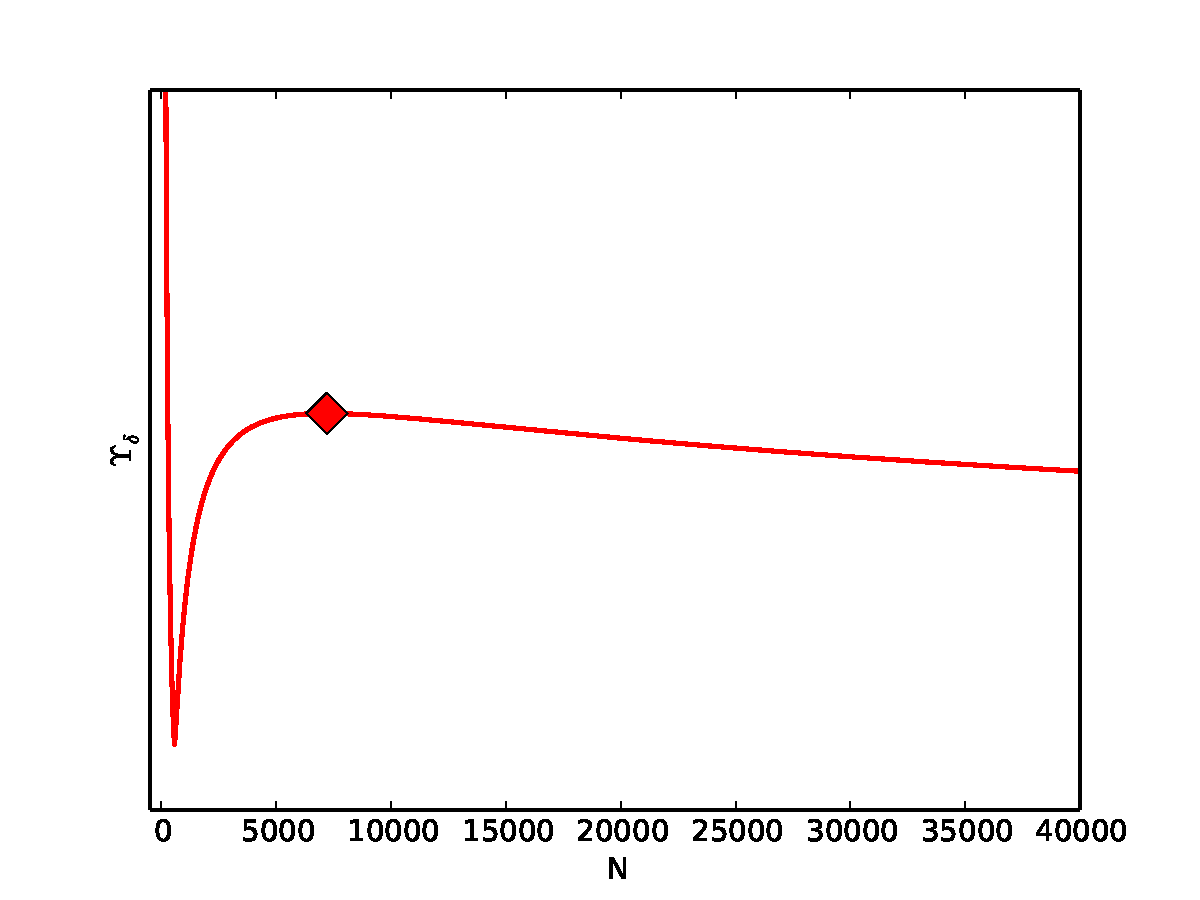
\includegraphics[width = \textwidth,center]{Images/upsilon.pdf}
\caption[Cost function $\Upsilon_\delta$ over batch size $N$.]{Cost function $\Upsilon_\delta$ over batch size $N$. The optimal batch size $N^*$ is marked with a diamond. Batch sizes under the global minimum $N_0$ do not guarantee any performance improvement.}
\label{fig:0}
\end{figure}

The main peculiarity of this result is that the step size is constant, in the sense that its value does not depend on the gradient estimate. This can be explained in terms of a duality between step size and batch size: in other conservative adaptive-step size approaches, such as the one proposed with Theorem \ref{theo:5}, the step size is kept small to counteract policy updates that are too off due to bad gradient estimates. When also the batch size is made adaptive, a sufficient number of sample trajectories can be taken to keep the policy update on track even with a constant-valued step size.
\paragraph{}
We now analyze this approach from a more algorithmic perspective.
As already mentioned, under Assumption \ref{assum:4}, Assumption \ref{assum:3} can be restated as:
\[
	N \geq N_0 \triangleq \frac{d_\delta^2}{\norm[\infty]{\gradApp{\vtheta}}^2},
\]
which is always verified by the proposed $N^*$. This means that the adaptive batch size never allows an estimation error larger than the gradient estimate. This is good news, but it may also lead to very high batch sizes once $\vtheta$ is very close to the optimal parameter. An additional stopping condition may be necessary, and one option is simply to set a maximum allowed batch size.
\paragraph{}
Notice also that the optimal batch size, as defined in Theorem \ref{theo:5}, is referred to the upcoming parameter update. However, the optimal batch size can be employed only for the next update, since trajectory samples need to be collected first. This means that, in any practical implementation, the adaptive batch size that we have defined is always "a learning iteration too late". However, it is reasonable to assume that the conditions that determined the optimal batch size will not vary significantly between a learning iteration and the following one. While we need to rely on $N$'s predictive power, we can keep the step size synchronized as follows: compute $\Lambda^*$ as in Corollary \ref{cor:3}, using:
\[
	\epsilon = \frac{d_\delta}{\sqrt{N}},
\]
where $d_\delta$ is computed with the latest available data and $N$ is the batch size used to collect them. A collateral effect of this approach is that, due to integer approximation, the step size is no longer constant. However, the variations in its value should be quite small.
\paragraph{}
These expedients lead to the following algorithm: 
\begin{algorithm}[H]
\caption{Adaptive Policy Gradient}
\label{alg:adabatch}
\begin{algorithmic}
\State set initial policy parametrization $\vtheta$
\State set initial batch size $N$ and maximum batch size $\overline{N}$
\State $c \gets 		\frac{RM_{\phi}^2}{(1-\gamma)^2\sigma^2}\left(\frac{|\mathcal{A}|}{\sqrt{2\pi}\sigma} +	\frac{\gamma}{2(1-\gamma)}\right)$
\State $\epsilon \gets 0$
\While{$\epsilon < |\gradApp{\vtheta}|$} 
\State perform $N$ trajectories following policy 
	$\pi_{\vtheta} \sim \mathcal{N}(\vtheta^T\vphi(s),\sigma)$
\State compute policy gradient estimate $\gradApp{\vtheta}$
\State $k \gets \arg\max_i|\gradApp{\theta_i}|$
\State compute $d_\delta$ with a proper concentration bound
\State $\epsilon \gets \nicefrac{d_\delta}{\sqrt{N}}$
\State $\alpha \gets \frac{
		\left(\norm[\infty]{\gradApp{\vtheta}} - \epsilon\right)^2}
		{2c
		\left(\norm[\infty]{\gradApp{\vtheta}} + \epsilon\right)^2}$
\State $\theta_k \gets \theta_k + \alpha\gradApp{\theta_k}$
\State $N \gets \left\lceil\frac{(13+3\sqrt{17})d_{\delta}^2}{2\norm[\infty]{\gradApp{\vtheta}}^2}\right\rceil$
\State $N \gets \max\{2,\min\{N,\overline{N}\}\}$
\EndWhile
\end{algorithmic}
\end{algorithm}

Notice that there is still a parameter that must be selected by an expert: $\delta$. This is the probability of having a worsening update, since monotonic improvement is guaranteed with probability $(1-\delta)^m$. Intuitively, the choice of $\delta$ depends on risk attitude and should be small in critical applications. However, numerical simulations (see Section \ref{sec:simul}) show that, at least for simple problems, $\delta$ can be set to very high values ($\sim 1$) without compromising monotonic improvement. This can be useful, since larger values of $\delta$ lead to faster convergence.

We now consider some concentration bounds in more detail, providing the values for $d_{\delta}$ and the corresponding explicit expressions for $N^*$.

\subsection{Chebyshev's bound}\label{sec:chebyshev}
We report here the sample mean version of Chebyshev's bound for a generic stochastic variable $X$:
\[
	\Pr(|E[X] - \overline{X}_N| \geq \epsilon) \leq \frac{Var[X]}{N},
\]
where $\overline{X}_N$ is the sample mean over $N$ samples.
In our case we have:
\[
	\delta = \Pr(|\gradJ{\theta_i} - \gradApp{\theta_i}| 
		\geq \epsilon) \leq \frac{Var[\gradApp{\theta_i}]}{N}.
\]
This bound is compliant with Assumption \ref{assum:4} and gives the following expression for $d_\delta$:
\[
d_\delta = \sqrt{\frac{Var[\gradSim{\theta_i}]}{\delta}},
\]
where $\gradSim{\theta_i}$ is the policy gradient approximator (from a single sample trajectory).
The main advantage of this bound is that it doesn't make any assumption on the range of the gradient sample.
\paragraph{}
Using results from \cite{DBLP:journals/nn/ZhaoHNS12} as adapted in \cite{NIPS2013_5186}, we can give explicit formulations for the optimal batch size.
When the REINFORCE \cite{Williams1992} gradient estimator ($\gradRF{\vtheta}$) is used to estimate the gradient, we can use Lemma 5.4 from \cite{NIPS2013_5186} to bound the estimation error as:

\[
\epsilon \leq \frac{1}{\sqrt{N}}\left(\frac{RM_{\phi}(1-\gamma^H)}
				{\sigma(1-\gamma)}\sqrt{\frac{H}{\delta}}\right),
\]

which gives an optimal batch size:
\[
N^* = \frac{(13+3\sqrt{17})R^2M_{\phi}^2H(1-\gamma^H)^2}
	 		{2\delta\sigma^2(1-\gamma)^2
	 			\norm[\infty]{\gradRF{\vtheta}}^2}.
\]
Similarly, when the G(PO)MDP/PGT gradient estimator ($\gradPGT{\vtheta}$) is used, using Lemma 5.5 from \cite{NIPS2013_5186} we have:

\[
\epsilon \leq \frac{1}{\sqrt{N}}\left(\frac{RM_{\phi}}
				{\sigma(1-\gamma)}\sqrt{\frac{1}{\delta}
				\left[\frac{1-\gamma^{2H}}{1-\gamma^2} + H\gamma^{2H} - 2\gamma^H
				\frac{1-\gamma^H}{1-\gamma}\right]}\right)
\]

and

\[
N^* = \frac{(13+3\sqrt{17})R^2M_{\phi}^2
			\left[\frac{1-\gamma^{2H}}{1-\gamma^2} + H\gamma^{2H} - 2\gamma^H
	 		\frac{1-\gamma^H}{1-\gamma}\right]}
	 		{2\delta\sigma^2(1-\gamma)^2
	 			\norm[\infty]{\gradPGT{\vtheta}}^2}.
\]
These results are independent from the baseline used in the gradient estimation. The G(PO)MDP/PGT estimator suffers from a smaller variance if compared with REINFORCE, and the variance bound is indeed tighter.

\subsection{Hoeffding's bound}
We report Hoeffding's bound applied to our case:
\[
	\delta = \Pr(|\gradJ{\theta_i} - \gradApp{\theta_i}| \geq \epsilon)
		 \leq 2e^{-\frac{2\epsilon^2}{N\mathbf{R}^2}},
\]
where $\mathbf{R}$ is the range of the gradient approximator, i.e. $|supp(\gradSim{\theta_i})|$.
This bound is compliant with Assumption \ref{assum:4} and gives:
\[
d_\delta = \mathbf{R}\sqrt{\frac{\log{2/\delta}}{2}},
\]
For the class of policies we are considering, i.e. Gaussian with mean linear in the features, the range can be upper bounded under some assumptions:

\begin{restatable}{lemma}{secondlemma}
For any Gaussian policy $\pi_\theta \sim \mathcal{N}(\vtheta^T\vphi(s),\sigma^2)$, assuming that the action space is bounded ($|a|\leq \overline{A}\:\:\forall a \in \mathcal{A}$) and the policy gradient is estimated on trajectories of length $H$,the range $\mathbf{R}$ of the policy gradient sample $\gradSim{\theta_i}$ can be upper bounded $\forall i=1,\dots,m$ and $\forall \theta$ by
\[
\mathbf{R} \leq \frac{2HM_{\phi}\overline{A}R}{\sigma^2(1-\gamma)}.
\]
\end{restatable}

As we will show in Section \ref{sec:simul}, a more practical solution (even if less rigorous) consists in computing the range as the difference between the largest and the smallest gradient sample seen during learning.

\subsection{Empirical Bernstein's bound}
Tighter concentration bounds allow for smaller batch sizes (which result in more frequent policy updates) and larger step sizes, thus speeding up the learning process and improving long-time average performance. An empirical Bernstein bound from \cite{Mnih:2008:EBS:1390156.1390241} allows to use sample variance instead of the variance bounds from \cite{DBLP:journals/nn/ZhaoHNS12} and to limit the impact of the gradient range. We report the bound for a generic stochastic variable $X$:
\[
	|E[X] - \overline{X}_N| \leq  \sqrt{\frac{2S_N\ln{\nicefrac{3}{\delta}}}{N}}
		+ \frac{3\mathbf{R}\ln{\nicefrac{3}{\delta}}}{N},
\]
where $S_N$ is the sample variance of $X$, defined as:
\[
	S_N = \frac{1}{N}\sum\limits_{i=1}^N(X_i - \overline{X}_N)^2.
\]
Unfortunately, this bound does not satisfy Assumption \ref{assum:4}, giving for the estimation error the following, more complex, expression:
 \[
 \epsilon(N) = \frac{d_\delta}{\sqrt{N}} + \frac{f_\delta}{N},
\]
where
\begin{align*}
d_\delta= \sqrt{2S_N\ln{\nicefrac{3}{\delta}}}, && f=3\mathbf{R}\ln{\nicefrac{3}{\delta}},
\end{align*}

No reasonably simple closed-form solution is available in this case, requiring a linear search of the batch size $N^*$ maximizing $\Upsilon_\delta$. 

The cost function to optimize becomes (already optimized w.r.t the step size):
\[
\Upsilon_{\delta}(\Lambda^*,N) = \frac{\left(\norm[\infty]{\gradApp{\vtheta}} - 
		\sqrt{\frac{2S_N\ln{\nicefrac{3}{\delta}}}{N}} - \frac{3\mathbf{R}\ln{\nicefrac{3}{\delta}}}{N}\right)^4}
		{4cN
		\left(\norm[\infty]{\gradApp{\vtheta}} + 
				\sqrt{\frac{2S_N\ln{\nicefrac{3}{\delta}}}{N}} + \frac{3\mathbf{R}\ln{\nicefrac{3}{\delta}}}{N}\right)^2}.
\]
First of all, Assumption \ref{assum:3} gives the following constraint:
\[
N \geq N_0 := \left(\frac{d_{\delta} + \sqrt{d_{\delta}^2 + 4f_{\delta}\norm[\infty]{\gradApp{\vtheta}}}}
{2\norm[\infty]{\gradApp{\vtheta}}}
\right)^2,
\]
so $N_0$ can be used as the starting point of the linear search.
Computing the derivative w.r.t $N$ we obtain two distinct factors for the numerator:

\begin{scriptsize}
\begin{align*}
&\left(d_{\delta}\sqrt{N}+f_{\delta} - \norm[\infty]{\gradApp{\vtheta}}N\right)^3, \\
&\left(2d_{\delta}^2N+5d_{\delta}f_{\delta}\sqrt{N}+3d_{\delta}\norm[\infty]{\gradApp{\vtheta}}N^{\nicefrac{3}{2}} +3f_{\delta}^2+6f\norm[\infty]{\gradApp{\vtheta}}N-\norm[\infty]{\gradApp{\vtheta}}^2N^2\right).
\end{align*}
\end{scriptsize}

The first one gives again $N_0$, which is the global minimum. By applying Descartes' rule of signs to the other one, seen as a polynomial in $\sqrt{N}$, we see that it gives just one root. The exact expression of this maximum is too big to be reported and too long to code, but its uniqueness, together with the fact that $\Upsilon_{\delta}$ goes to $0$ as N goes to infinity, justifies the following methodology: to find $N^*$, start from $N_0$ and stop as soon as the value of the cost function $\Upsilon(\Lambda^*,N)$ begins to decrease.
\paragraph{}
Note also that the optimal step size is no longer constant: it can be computed with the expression given in Corollary \ref{cor:3} by setting $\epsilon := \epsilon(N^*)$.
Finally, as for the Hoeffding's bound, the range $\mathbf{R}$ can be upper bounded exactly or estimated from samples.


	\chapter{Numerical simulations}\label{sec:simul}

In this chapter we conduct some experiments to test our safe method. We compare the different variants of our algorithm to observe their performance in practice. We also compare our method with older or more common approaches to see how much the theoretical improvements obtained in the previous chapter translate into better practical results.

In Section \ref{sec:lqg1d} we use a simple simulated control task, one-dimensional \ac{LQG}, to compare the different variants of our algorithm.
In Section \ref{sec:lqg2d} we use a two-dimensional variant of the same problem to show the advantages of our method over older approaches.
In Section \ref{sec:cartpole} we use a continuous action variant of the popular cart-pole task to improve a baseline policy after a change has been introduced to the environment, to show the practical advantages of our method.

\section{One-Dimensional LQG}\label{sec:lqg1d}
In this section we test the proposed methods on the one-dimensional \ac{LQG} problem \cite{4867}. We use this task as a testing ground because it is simple, all the constants involved in our bounds can be computed exactly, and the optimal parameter $\theta^*$ is available as a reference.

The LQG problem is a continuous \ac{MDP} defined by transition model:
\[
	s_t \sim \mathcal{N}(s_t+a_t,\sigma_0^2),
\] 

reward function:
\[
	r_t=-0.5(s_t^2+a_t^2),
\]
and Gaussian policy:
\[
	a_t \sim \mathcal{N}(\theta\cdot s_t,\sigma^2).
\]
Intuitively, the problem is to bring to zero a system's state, in the presence of noise, with a cost for acting on the system.
The policy has a single parameter $\theta$. The optimal value $\theta^*$ can be computed exactly, but the problem can be used as a benchmark for \ac{RL} algorithms.

In all our simulations we use $\sigma_0 = 0$, since all the noise can be modeled on the agent's side without loss of generality. Both action and state variables are bounded to the interval $[-2,2]$ and the initial state is drawn uniformly at random.  
We use a discount factor $\gamma=0.9$, which gives as optimal parameter $\theta^* \approx -0.59$, corresponding to expected performance $J(\theta^*) \approx -13.21$. The expected performance is very pessimistic, since it doesn't take into account the bound on actions and states and the limited length of the task horizon, but equally captures the progress of the real performance. A monotonically improving expected performance is a guarantee that the policy is improving without oscillation, even if the measured performance is noisy due to stochasticity in the environment and in the policy itself.
\paragraph{}
In our experiments, we are interested both in the convergence speed and in policy oscillation. We call \textit{improvement ratio} the ratio of policy updates that does not result in a worsening of the expected performance. First of all, we want to analyze how the choice of fixed step sizes and batch sizes may affect the improvement ratio and how much it depends on the variability of the trajectories (that in this case is due to the variance of the policy $\sigma$).
Table \ref{tab:1} shows the improvement ratio for two parameterizations ($\sigma=0.5$ and $\sigma=1$) when various constant step sizes and batch sizes are used, starting from $\theta=-0.55$ and stopping after a total of one million trajectories. 

\begin{table}[H]
\caption[Improvement ratio of the policy updates for different parametrizations of the LQG task.]{Improvement ratio of the policy updates for different policy standard deviation $\sigma$, fixed batch size $N$ and fixed step size $\alpha$, using the G(PO)MDP gradient estimator.}
\label{tab:1}
\centering
\begin{adjustbox}{width=1.0\linewidth,center}
\begin{tabular}{@{}llccccccc@{}} 
\toprule
\phantom{abc} & \phantom{abc} & \multicolumn{3}{c}{$\sigma=0.5$} & \phantom{abc} & \multicolumn{3}{c}{$\sigma=1$} \\
\cmidrule{3-5} \cmidrule{7-9}
\phantom{abc} & \phantom{abc} & $N=10000$ & $N=1000$ & $N=100$ & \phantom{abc} & $N=10000$ & $N=1000$ & $N=100$
\\\cmidrule{3-9}
\phantom{abc} & 1e-3 & 95.96\% & 52.85\% & 49.79\% & \phantom{abc} & 24.24\% & 37.4\% & 50.4\% \\ 
 $\alpha$	  & 1e-4 & 100\% & 73.27\% & 51.41\% & \phantom{abc} & 100\% & 27.03\% & 46.08\% \\
\phantom{abc} & 1e-5 & 98.99\% & 81.88\% & 55.69\% & \phantom{abc} & 100\% & 99.9\% & 39.04\%\\
\phantom{abc} & 1e-6 & 100\% & 83.88\% & 58.44\% & \phantom{abc} & 100\% & 100\% & 86.04\% \\
\bottomrule
\end{tabular}
\end{adjustbox}
\end{table}

As expected, small batch sizes combined with large step sizes lead to low improvement ratios. However, the effect of the meta-parameters is non-trivial and problem-dependent, justifying the need for an adaptive method.  
\paragraph{}
We now proceed to test the methods described in Chapter \ref{chap:main}. 
In all the following simulations we use $\sigma = 1$ and start from $\theta=0$, stopping after a total of 30 million trajectories.

We start by testing Algorithm \ref{alg:adabatch} with Chebyshev's bound as proposed in Section \ref{sec:chebyshev}. To estimate the gradient, we use the REINFORCE and G(PO)MDP gradient estimators. In both cases, we use optimal baseline from \cite{4867}.
Figure \ref{fig:1} shows the expected performance over sample trajectories for the two gradient estimators and for different values of $\delta$, the probability with which worsening updates are allowed to take place.

 To make this and the following figures more interpretable, some words must be spent on how data were processed. Each learning iteration corresponds to a single value of $\theta$, with a corresponding expected performance. The latter was scaled over time, simply by maintaining the value for all the trajectories of the batch (a closer look to the plot would reveal a series of steps of variable length and height). The horizontal scaling was performed to better capture the improvement of performance over time.


\begin{figure}[h!]
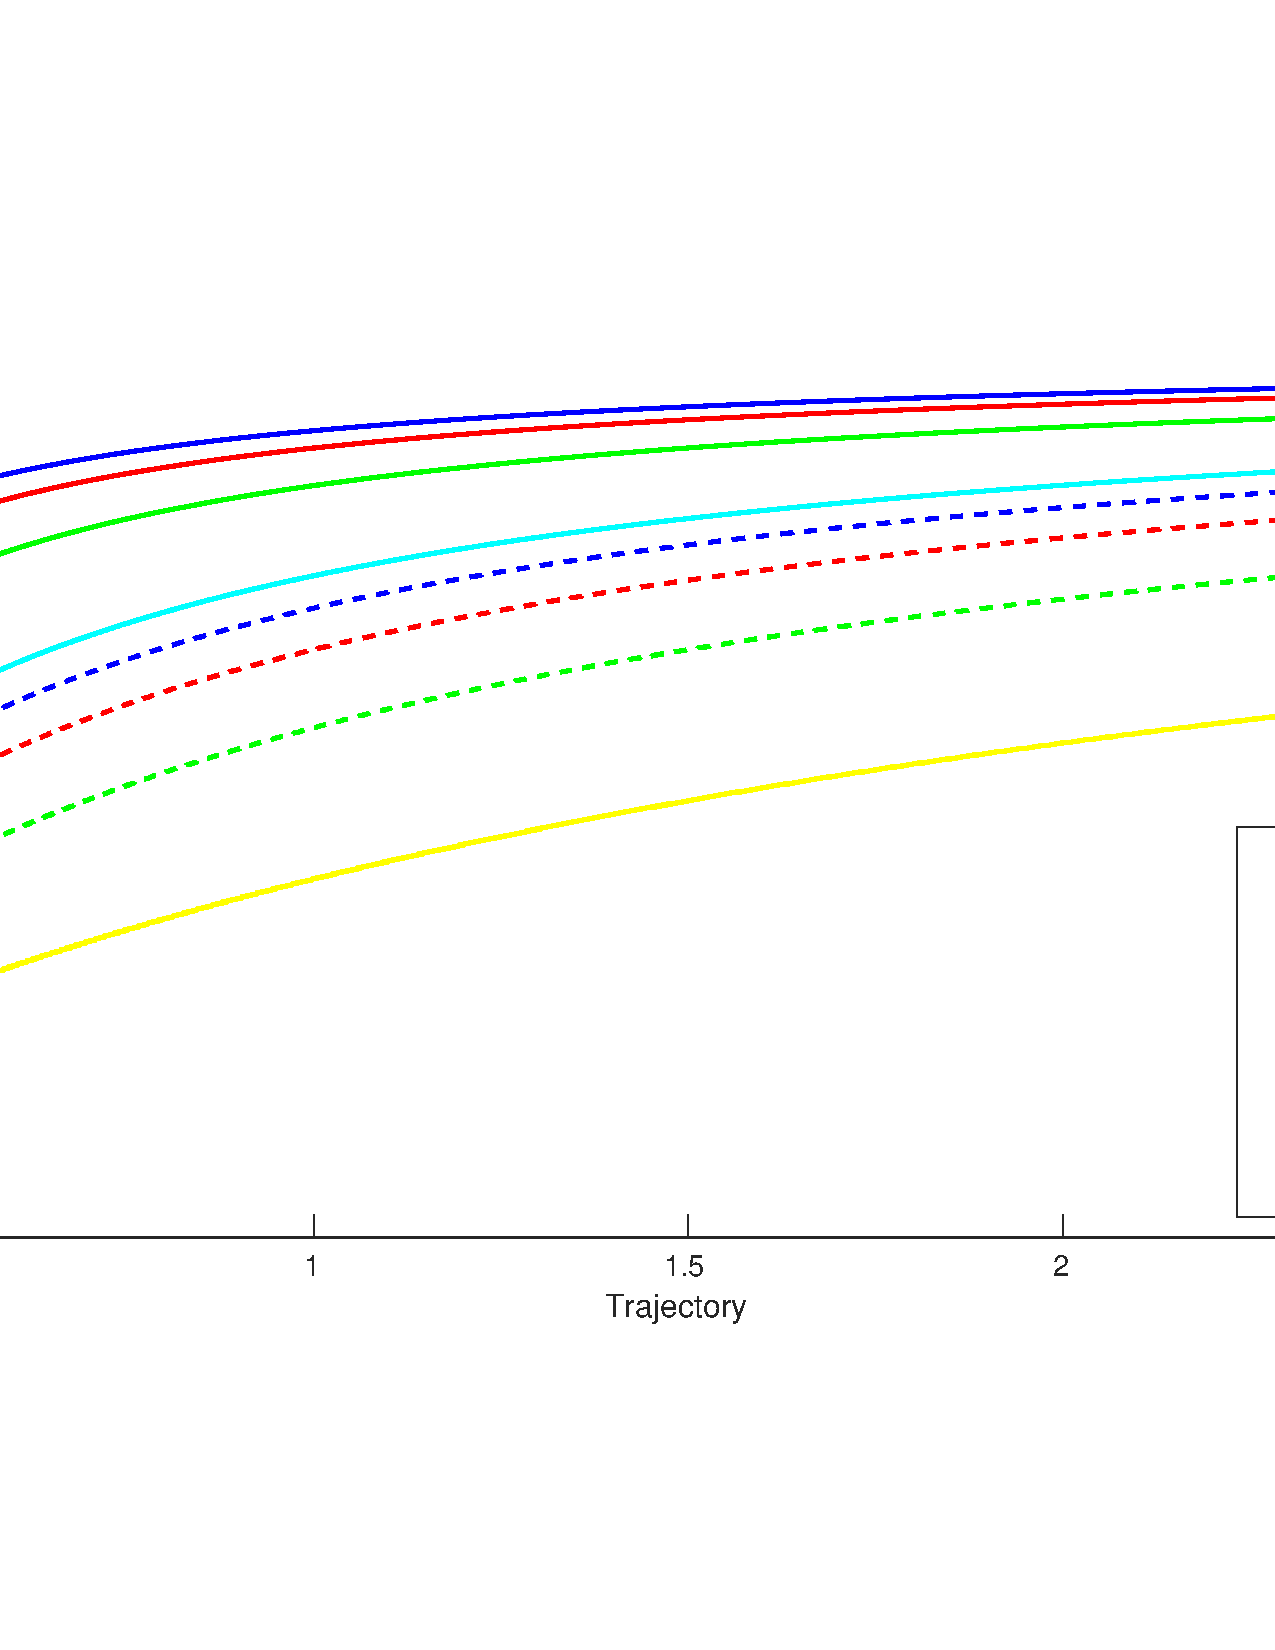
\includegraphics[width = \textwidth]{Images/chebyshev.pdf}
\caption[Expected performance over sample trajectories in the one-dimensional LQG task for different gradient estimators ad values of $\delta$.]{Expected performance over sample trajectories in the one-dimensional \ac{LQG} task, using G(PO)MDP and REINFORCE (dashed) gradient estimators and Chebyshev bound, for different values of $\delta$. Expected performance is computed for each parameter update. Data are then scaled to account for the different batch sizes. All results are averaged over 5 runs of 30 million total trajectories each.}
\label{fig:1}
\end{figure}

In general REINFORCE performs worse than G(PO)MDP due to its larger variance.
Larger values of $\delta$  lead to better performance. Notice that an improvement ratio of $1$ is achieved also with large values of $\delta$. This is due to the fact that the bounds used in the development of our method are not tight. Being the method this conservative, in practical applications $\delta$ can be set to a high value to improve the convergence rate.
\paragraph{}
The next step is to compare the Chebyshev's bound approach to the other methods proposed in Section \ref{sec:batchsize}. We stick to the configuration that performed the best in the previous experiment: G(PO)MDP to estimate the gradient and $\delta=0.95$. 
Figure \ref{fig:2} compares the performance of the different concentration bounds.

\begin{figure}[h!]
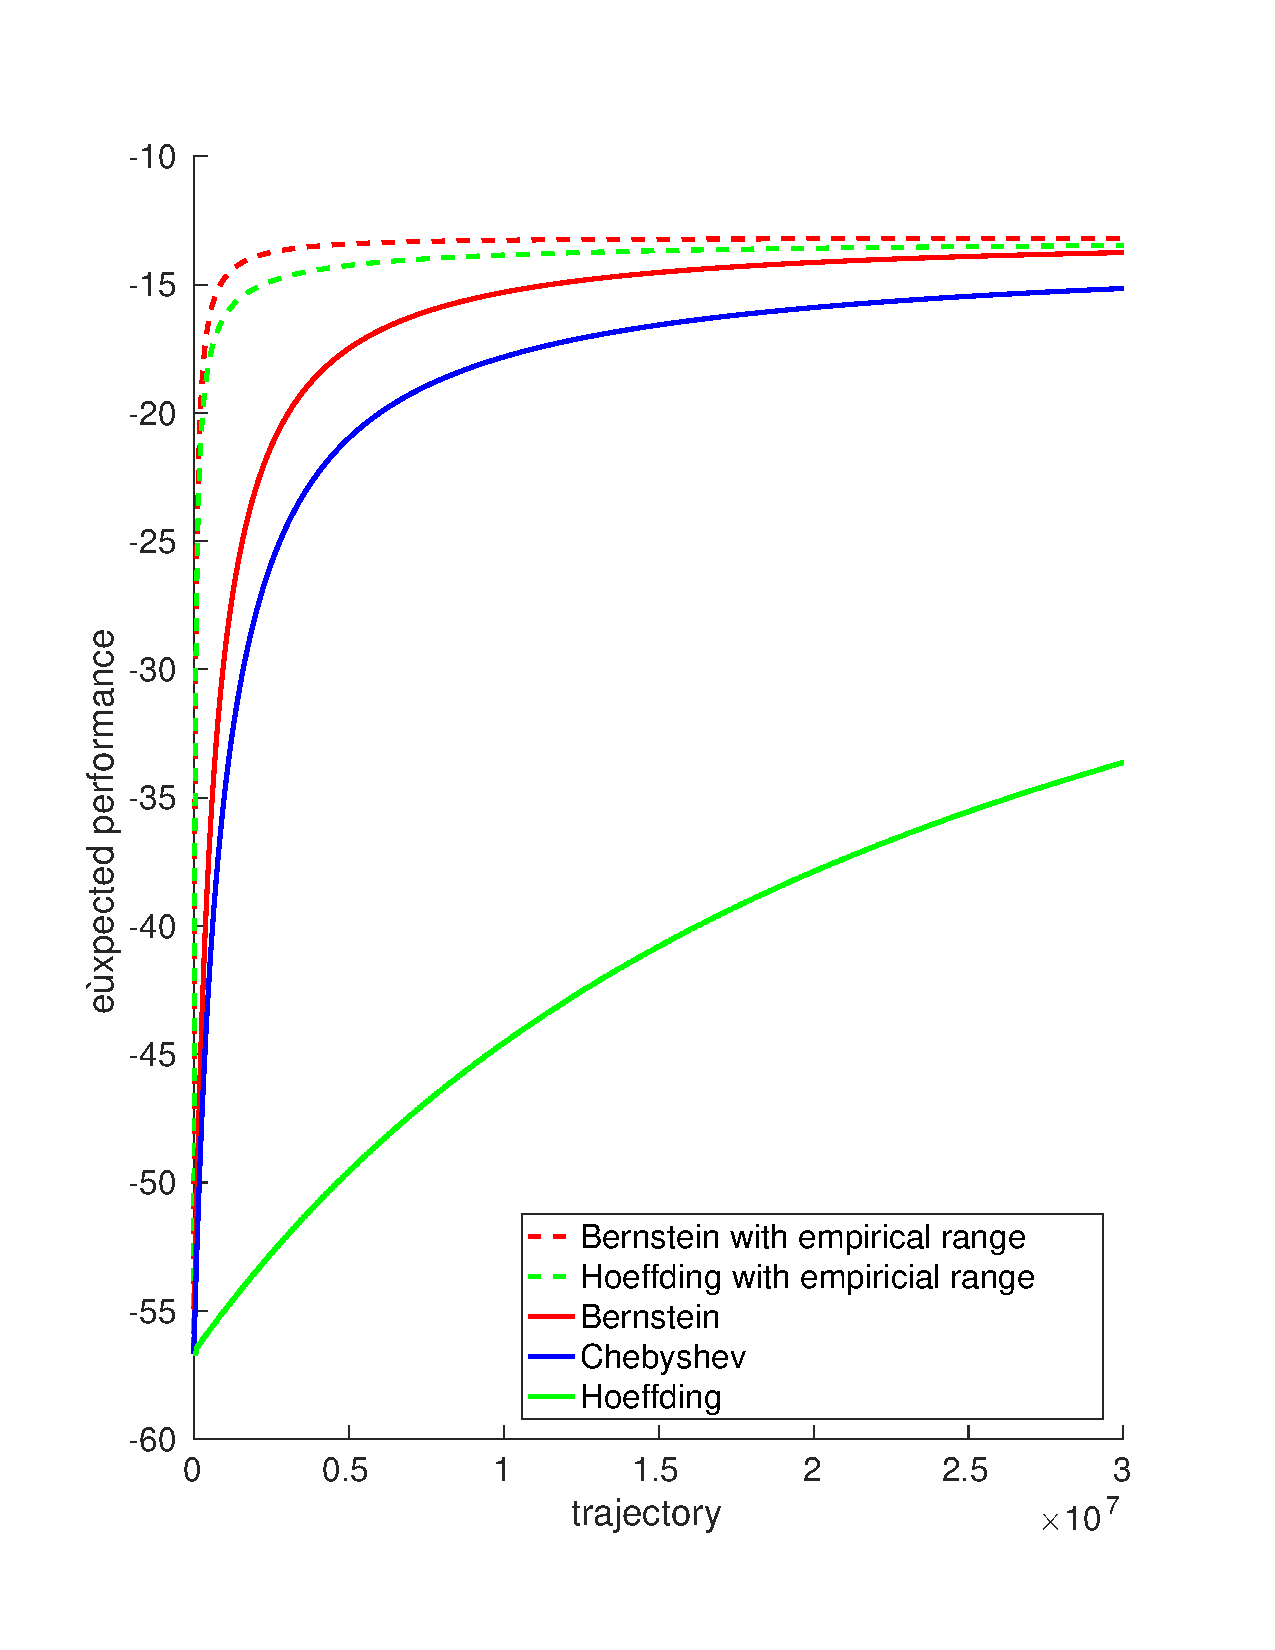
\includegraphics[width = 1.0\textwidth]{Images/compare_bounds.pdf}
\caption[Comparison of the performance of different statistical bounds in the one-dimensional LQG task.]{Comparison of the performance of different statistical bounds in the one-dimensional \ac{LQG} task, using the G(PO)MDP gradient estimator and $\delta=0.95$. All results are averaged over 5 runs.}
\label{fig:2}
\end{figure}

As expected, Bernstein's bound performs better than Chebyshev's, especially in the empirical range version. The rigorous version of Hoeffding's bound performs very poorly, while the one using the empirical range is almost as good as the corresponding Bernstein method. This is due to the fact that the bound on the gradient estimate range is very loose, since it accounts also for unrealistic combinations of state, action and reward.
\paragraph{}
To better capture the performance of the different variants of the algorithm in a real-time scenario, we define a metric $\overline{\Upsilon}$, which is obtained by averaging the real performance (measured during learning) over all the trajectories, coherently with the cost function used to derive the optimal batch size. The results are reported in Table \ref{tab:2}.

\begin{table}[H]
\caption[Average performance in the one-dimensional LQG task for different gradient estimators, statistical bounds and values of $\delta$.]{Average performance in the one-dimensional \ac{LQG} task for different gradient estimators, statistical bounds and values of $\delta$. All results are averaged over 5 runs ($5\%$ confidence intervals are reported). The abbreviation 'e.r.' stands for 'empirical range'}
\label{tab:2}
\centering
\begin{adjustbox}{width=1.0\linewidth,center}
\begin{tabular}{llccc}
\toprule
Estimator & Bound &$\delta$ & $\overline{\Upsilon}$ & Confidence interval \\\midrule 
\csvreader[head to column names]{Data/lqg_performance.csv}{}
{\\\csvcoli&\csvcolii&\csvcoliii&\csvcoliv&\csvcolv}
\\\bottomrule
\end{tabular}
\end{adjustbox}
\end{table}

Finally, it is interesting to look at the trend of the batch size over learning iterations. Figures \ref{fig:3} and \ref{fig:8} show the trend of the batch size for the different concentration bounds.

\begin{figure}[h!]
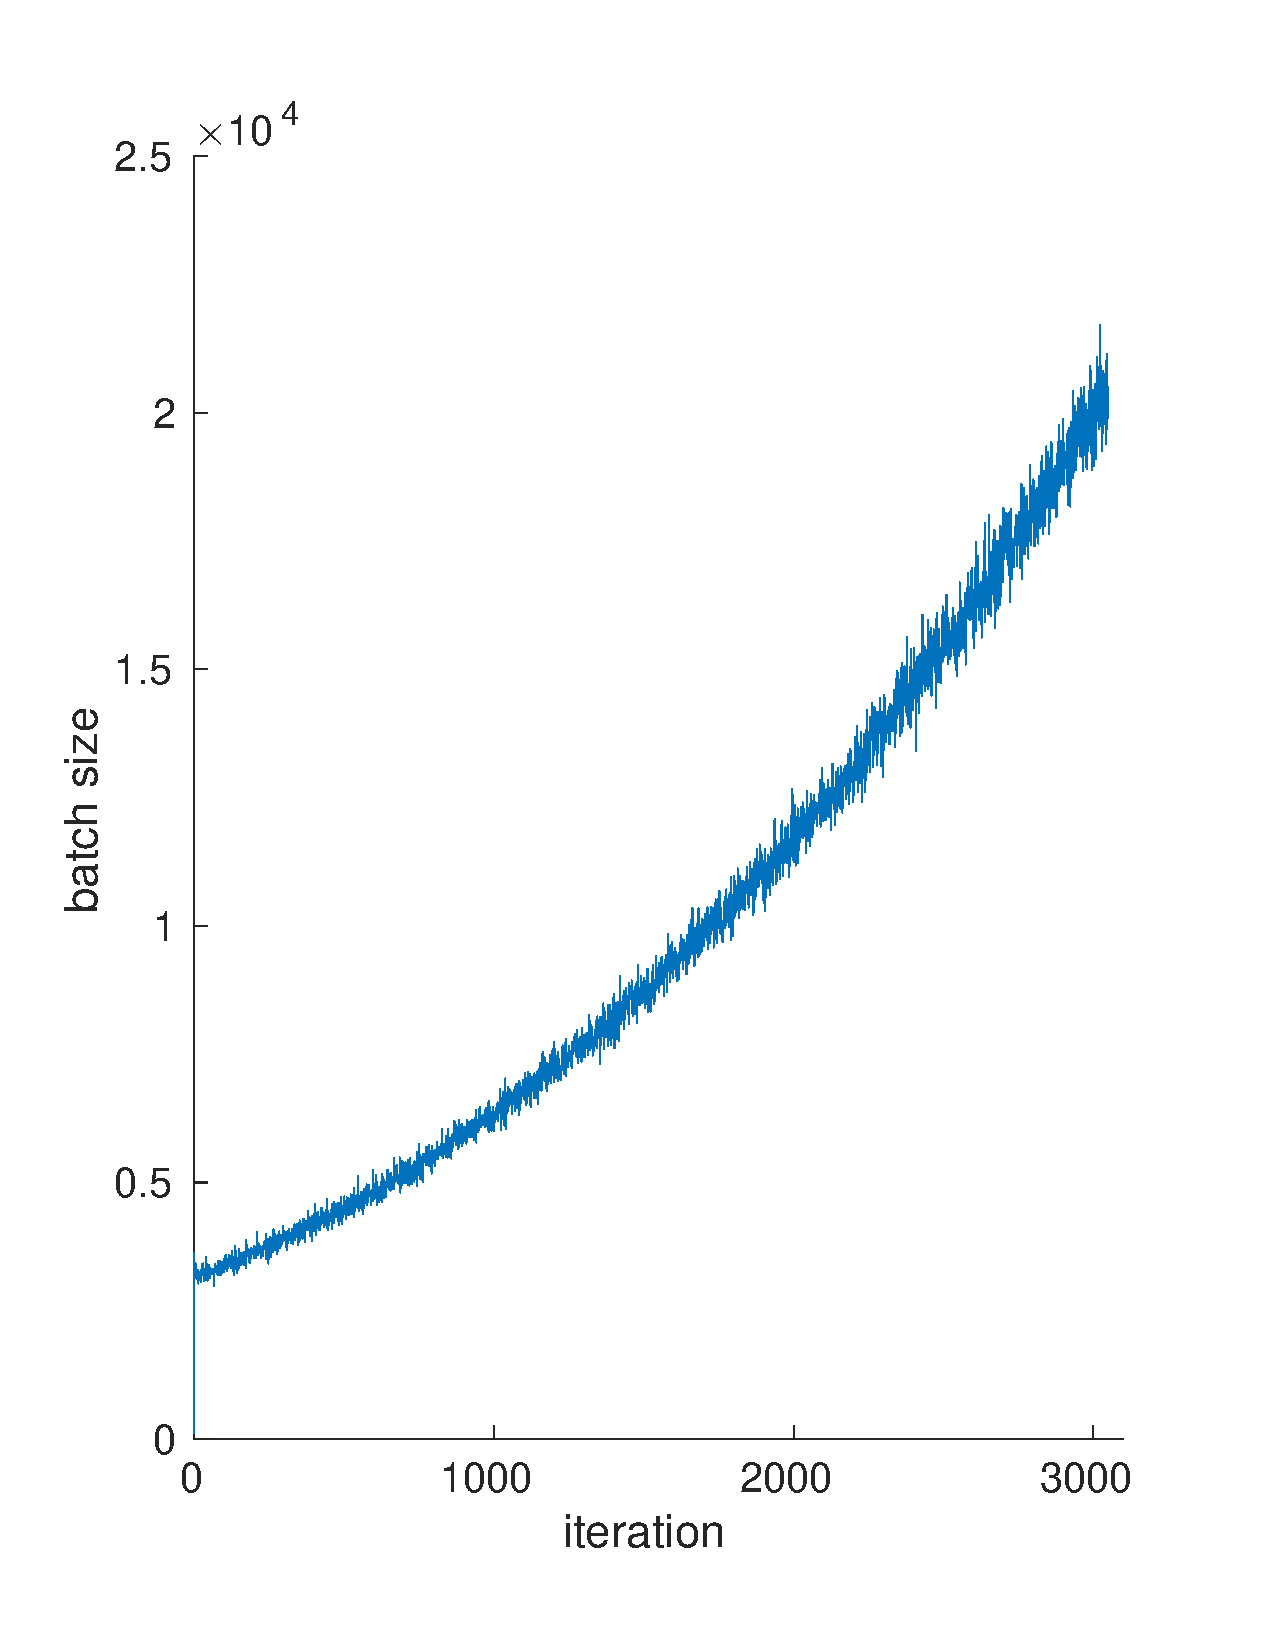
\includegraphics[width = \textwidth]{Images/batchsize_cheb.pdf}
\caption[Adaptive batch size over learning iterations in the one-dimensional LQG task using Chebyshev's bound.]{Adaptive batch size over learning iterations in the one-dimensional \ac{LQG} task, using the G(PO)MDP gradient estimator, Chebyshev's bound and $\delta=0.95$.}
\label{fig:3}
\end{figure}

\afterpage{
\begin{figure}[h!]
\begin{adjustbox}{center}
	\subfloat[Hoeffding]{
	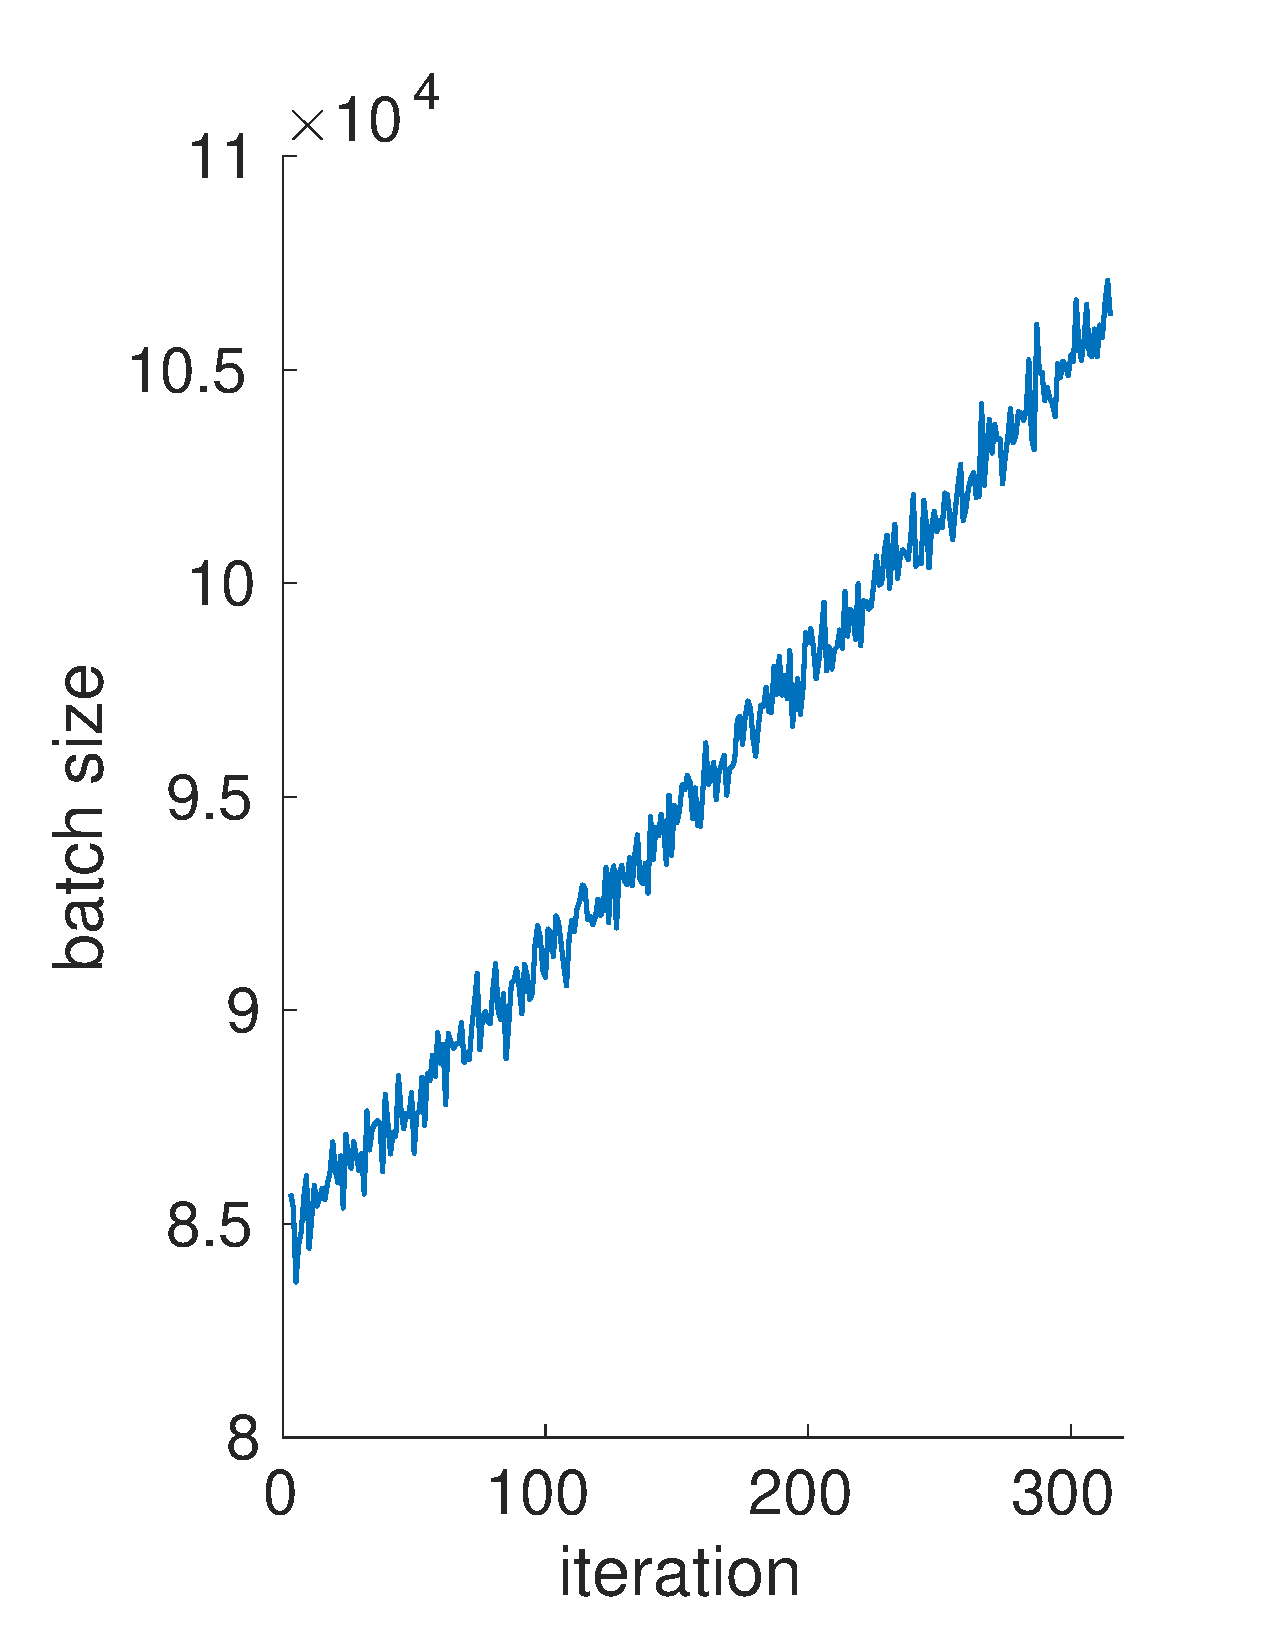
\includegraphics[width = 0.5\linewidth]{Images/batchsize_hoeff.pdf}
	\label{fig:4}
	}
	\subfloat[Hoeffding with empirical range]{
	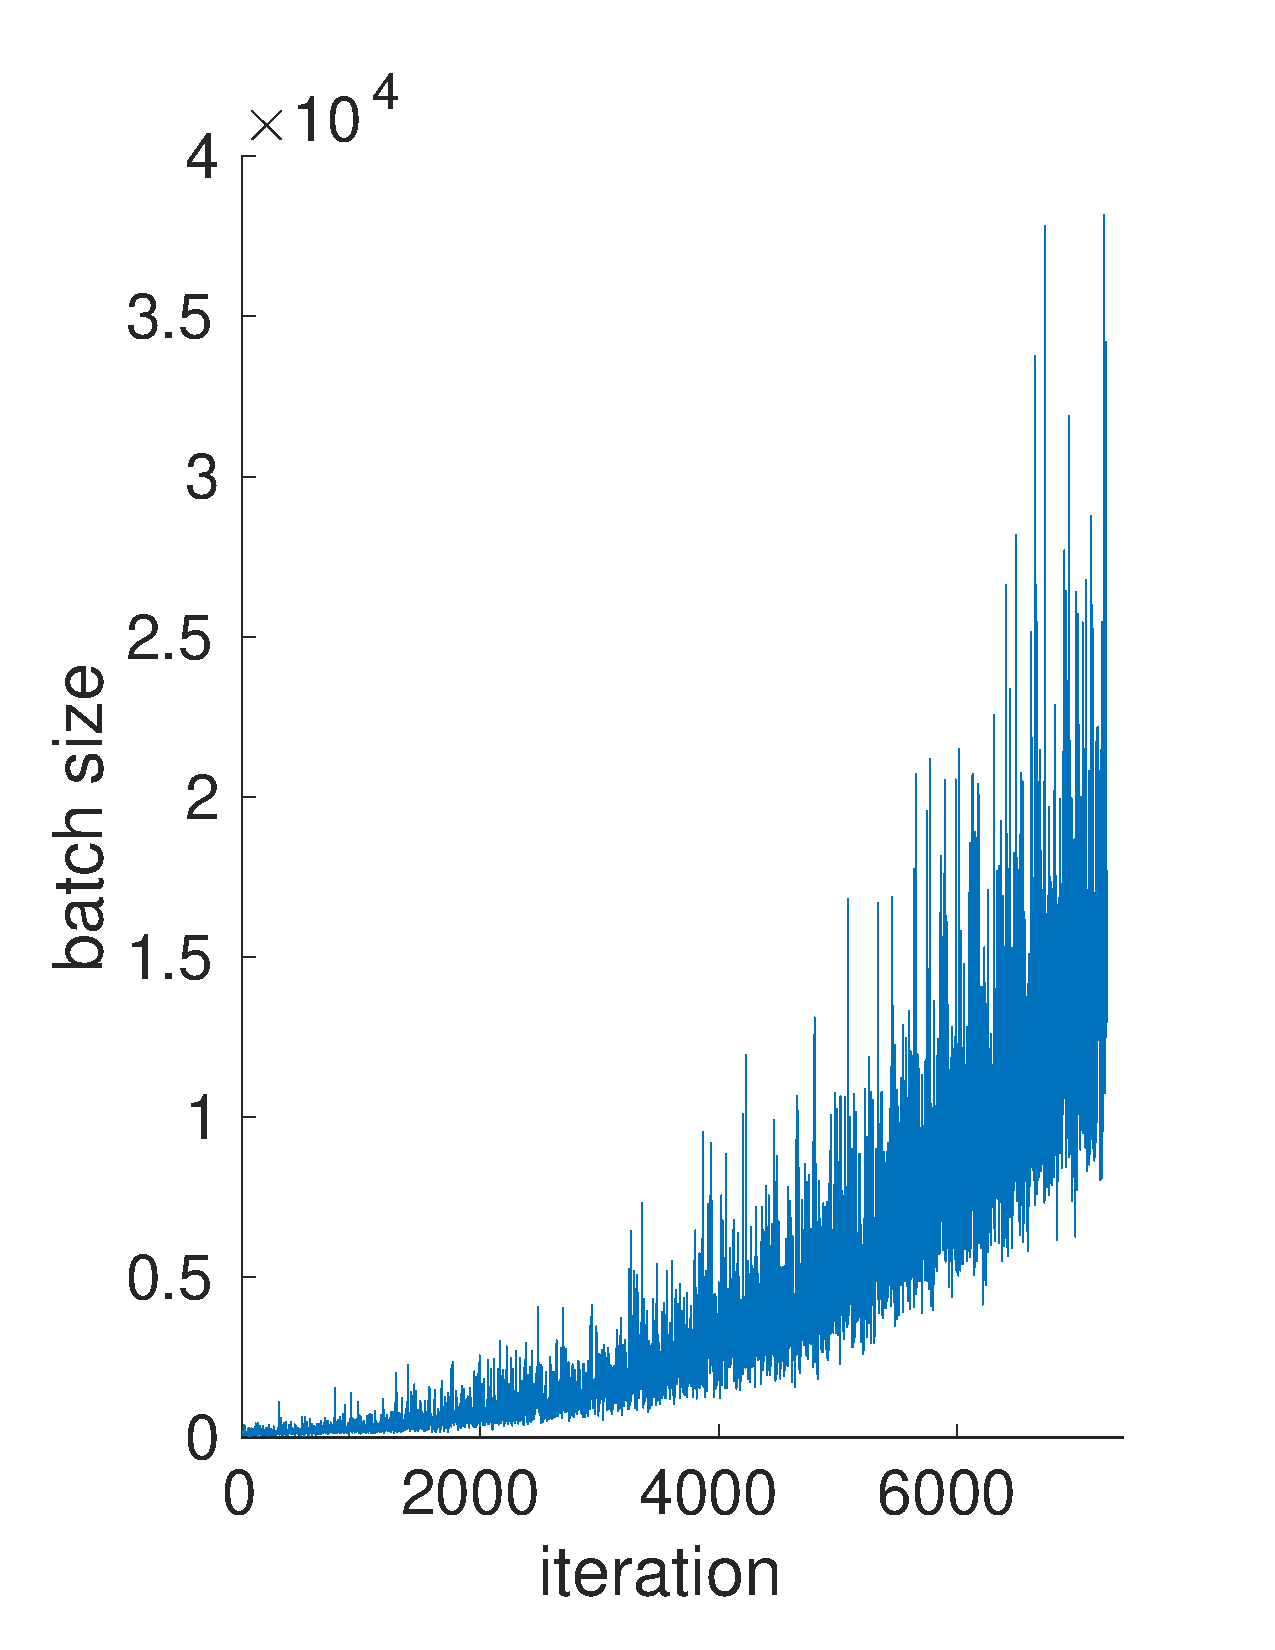
\includegraphics[width = 0.5\linewidth]{Images/batchsize_hoeff_emp.pdf}
	\label{fig:5}
	}
\end{adjustbox}
\begin{adjustbox}{center}
	\subfloat[Bernstein]{
	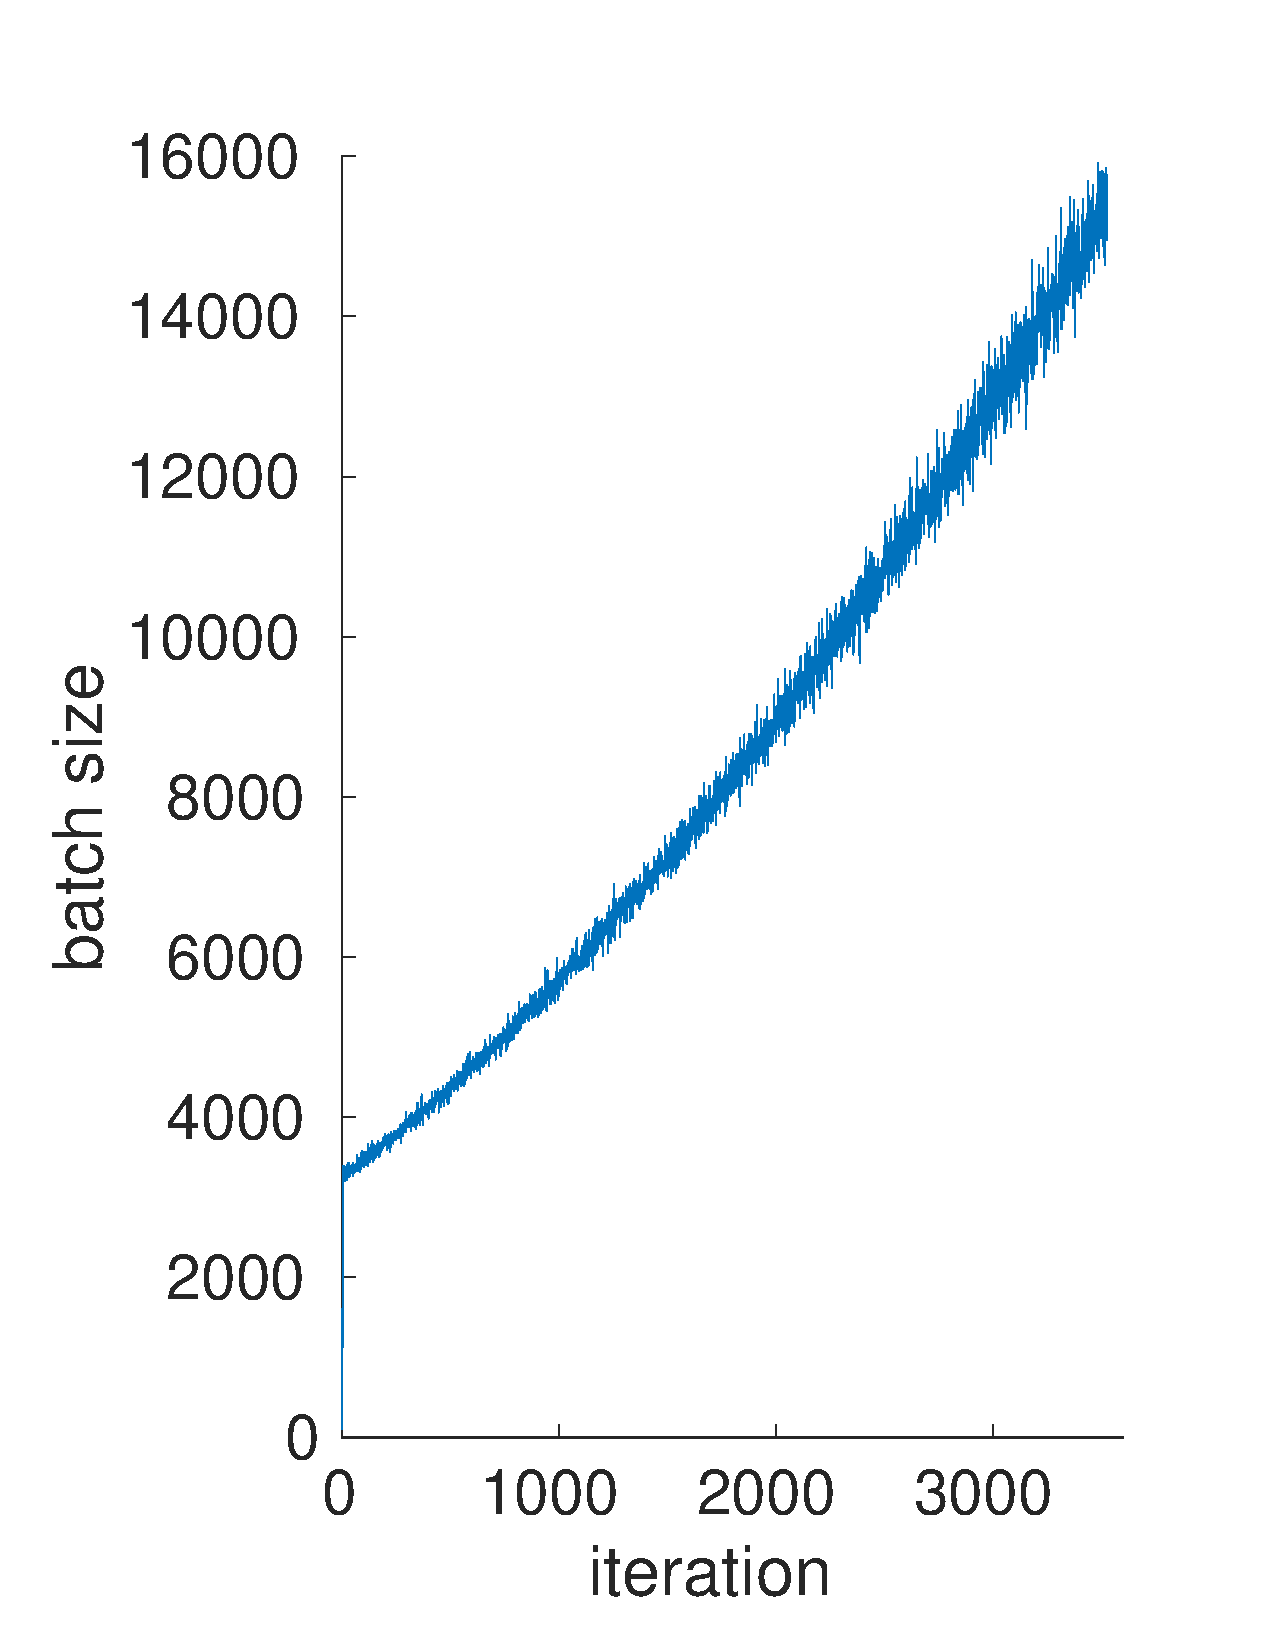
\includegraphics[width = 0.5\linewidth]{Images/batchsize_bern.pdf}
	\label{fig:6}
	}
	\subfloat[Bernstein with empirical range]{
	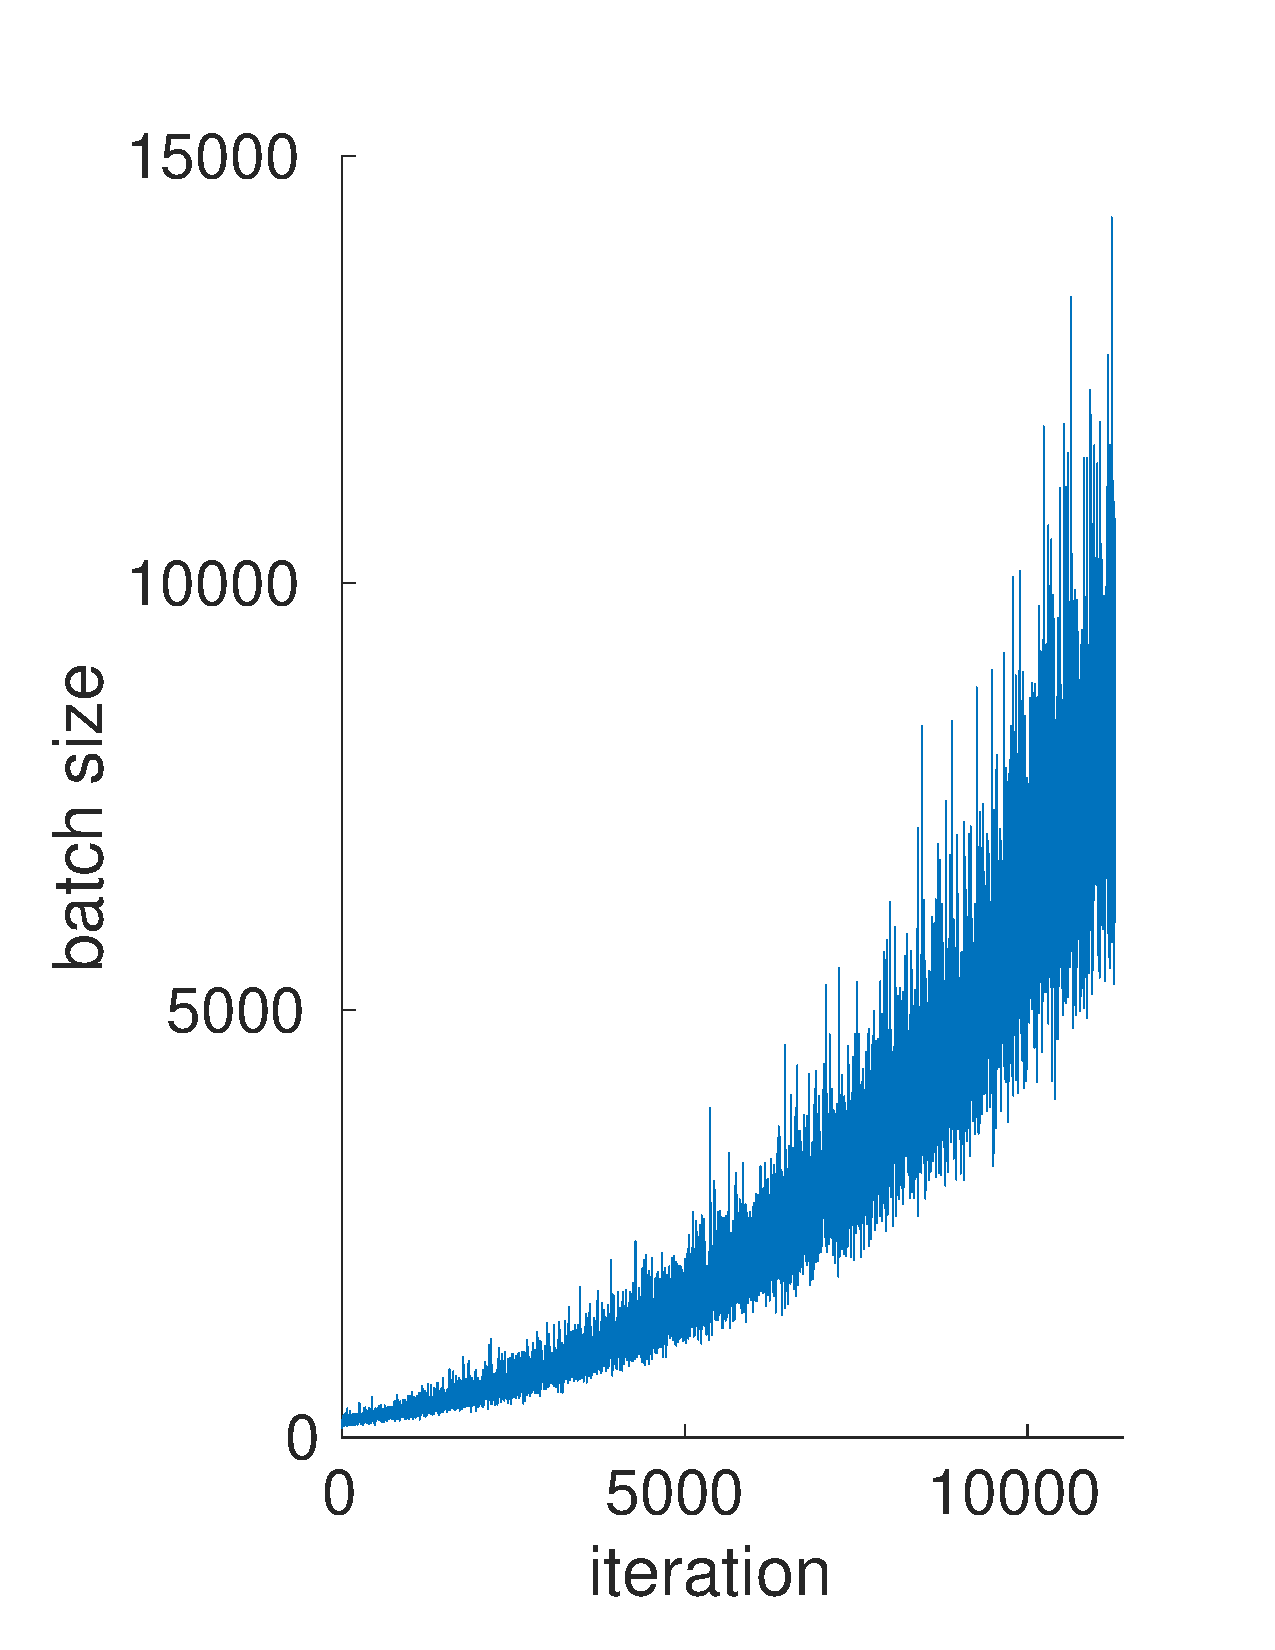
\includegraphics[width = 0.5\linewidth]{Images/batchsize_bern_emp.pdf}
	\label{fig:7}
	}
\end{adjustbox}

\caption[Adaptive batch size over learning iterations in the one-dimensional LQG task for different concentration bounds.]{Adaptive batch size over learning iterations in the one-dimensional \ac{LQG} task for different concentration bounds. In all the cases, the G(PO)MDP gradient estimator and $\delta=0.95$ were used.}
\label{fig:8}
\end{figure}
\clearpage
}

As expected, the batch size increases as the optimal parameter is approached, since positive improvements require more and more accuracy. The trend is evidently superlinear, with the exception of Hoeffding's bound with the theoretical range bound, which however selects very high batch sizes from the beginning. 

In all the experiments, the step size $\alpha$ is of the order of $10^{-6}$ and does not change significantly over learning iterations.


\section{Multi-dimensional LQG}\label{sec:lqg2d}
The one-dimensional \ac{LQG} problem was a good benchmark to compare the performance of different concentration bounds, but does not capture at all the coordinate descent aspect of our algorithm. Luckily, \ac{LQG} can easily be generalized to any number of dimensions $m$.

Following the approach of \cite{Pirotta:2015:MRL:2888116.2888124}, we define multi-dimensional \ac{LQG} as an \ac{MDP} with transition model:
\[
	\boldsymbol{s}_{t+1} \sim \mathcal{N}(\boldsymbol{s}_t+\boldsymbol{a}_t,C_0),
\] 

reward function:
\[
	r_t=-0.5(\boldsymbol{s}_t^TQ\boldsymbol{s}_t + \boldsymbol{a}_t^TR\boldsymbol{a}_t),
\]
and Gaussian policy:
\[
	\boldsymbol{a_t} \sim \mathcal{N}(\vtheta \cdot \boldsymbol{s}_t,C),
\]
where both $\boldsymbol{s}$ and $\boldsymbol{a}$ are vectors of size $m$, $C_0$ and $C$ are covariance matrices, $Q$ is a semidefinite matrix and $R$ is a symmetric positive definite matrix. All the matrices are $m\times m$. Note that also $\theta$ is an $m \times m$ matrix:
\[
\vtheta = \begin{bmatrix}
\theta_{11} & \theta_{12} \\
\theta_{21} & \theta_{22}.
\end{bmatrix}
\]
Similarly to the one-dimensional case, we set $C_0=\boldsymbol{0}$ without loss of generality. Matrices $Q$ and $R$ can be used to define different objectives.

\subsection{Independent action in two dimensions}
By setting $Q$ and $R$ to the identity matrix and using a diagonal covariance $C$, the result are two simultaneous, independent one-dimensional \ac{LQG} problems. Although this fact is intuitive, it may not be trivial for a learning algorithm to exploit it. In particular, we consider the two dimensional case ($m=2$), with covariance matrix:
\[
	C = 
	\begin{bmatrix}
	\sigma_1 & 0 		\\
	0		 & \sigma_2
	\end{bmatrix}.
\]
In particular, in our experiments, we use $\sigma_1 = \sigma_2 = 1$ and $\gamma = 0.95$. With these parameters, the optimal parameter matrix is (approximately):
\[
	\vtheta^* \simeq 
	\begin{bmatrix}
	-0.588 & 0 		\\
	0		 & -0.588
	\end{bmatrix},
\]
with corresponding expected performance $J_\mu(\vtheta^*) \simeq -422.616$. The fact that $\vtheta$ is diagonal is due precisely to the independence of the two one-dimensional \ac{LQG} tasks.

We first use this task to provide empirical evidence to the claim of Corollary \ref{cor:2}, \ie to show that the adaptive step size that we proposed is an improvement over the existing result that we generalized. We run two simulations, one with the scalar adaptive step size $\hat{\alpha}^*$ proposed in \cite{NIPS2013_5186}, which we report below, and one with the non-scalar adaptive step size $\Lambda^*$ of Corollary \ref{cor:3}:

\[
\hat{\alpha}^* =
	\frac{(1-\gamma)^3\sqrt{2\pi}\sigma^3
		\norm[2]{\gradDown{\vtheta}}^2}
		{(\gamma\sqrt{2\pi}\sigma)+2(1-\gamma)|\mathcal{A}|)RM_{\phi}^2
		\norm[1]{\gradUp{\vtheta}}^2}.	
\]

In both the simulations we use the G(PO)MDP gradient estimator with variance-minimizing baseline, Chebyshev's bound, $\delta=0.95$ and fixed batch size $N=2000$. We start from $\vtheta = \underline{0}$ and stop after a total of 30 million trajectories. The selected batch size happens to satisfy Assumption \ref{assum:3} for the duration of the experiment. This is necessary to preserve the performance improvement guarantee in both settings.
Figure \ref{fig:12} shows the expected performance over trajectories for the two experiments.

\begin{figure}[h!]
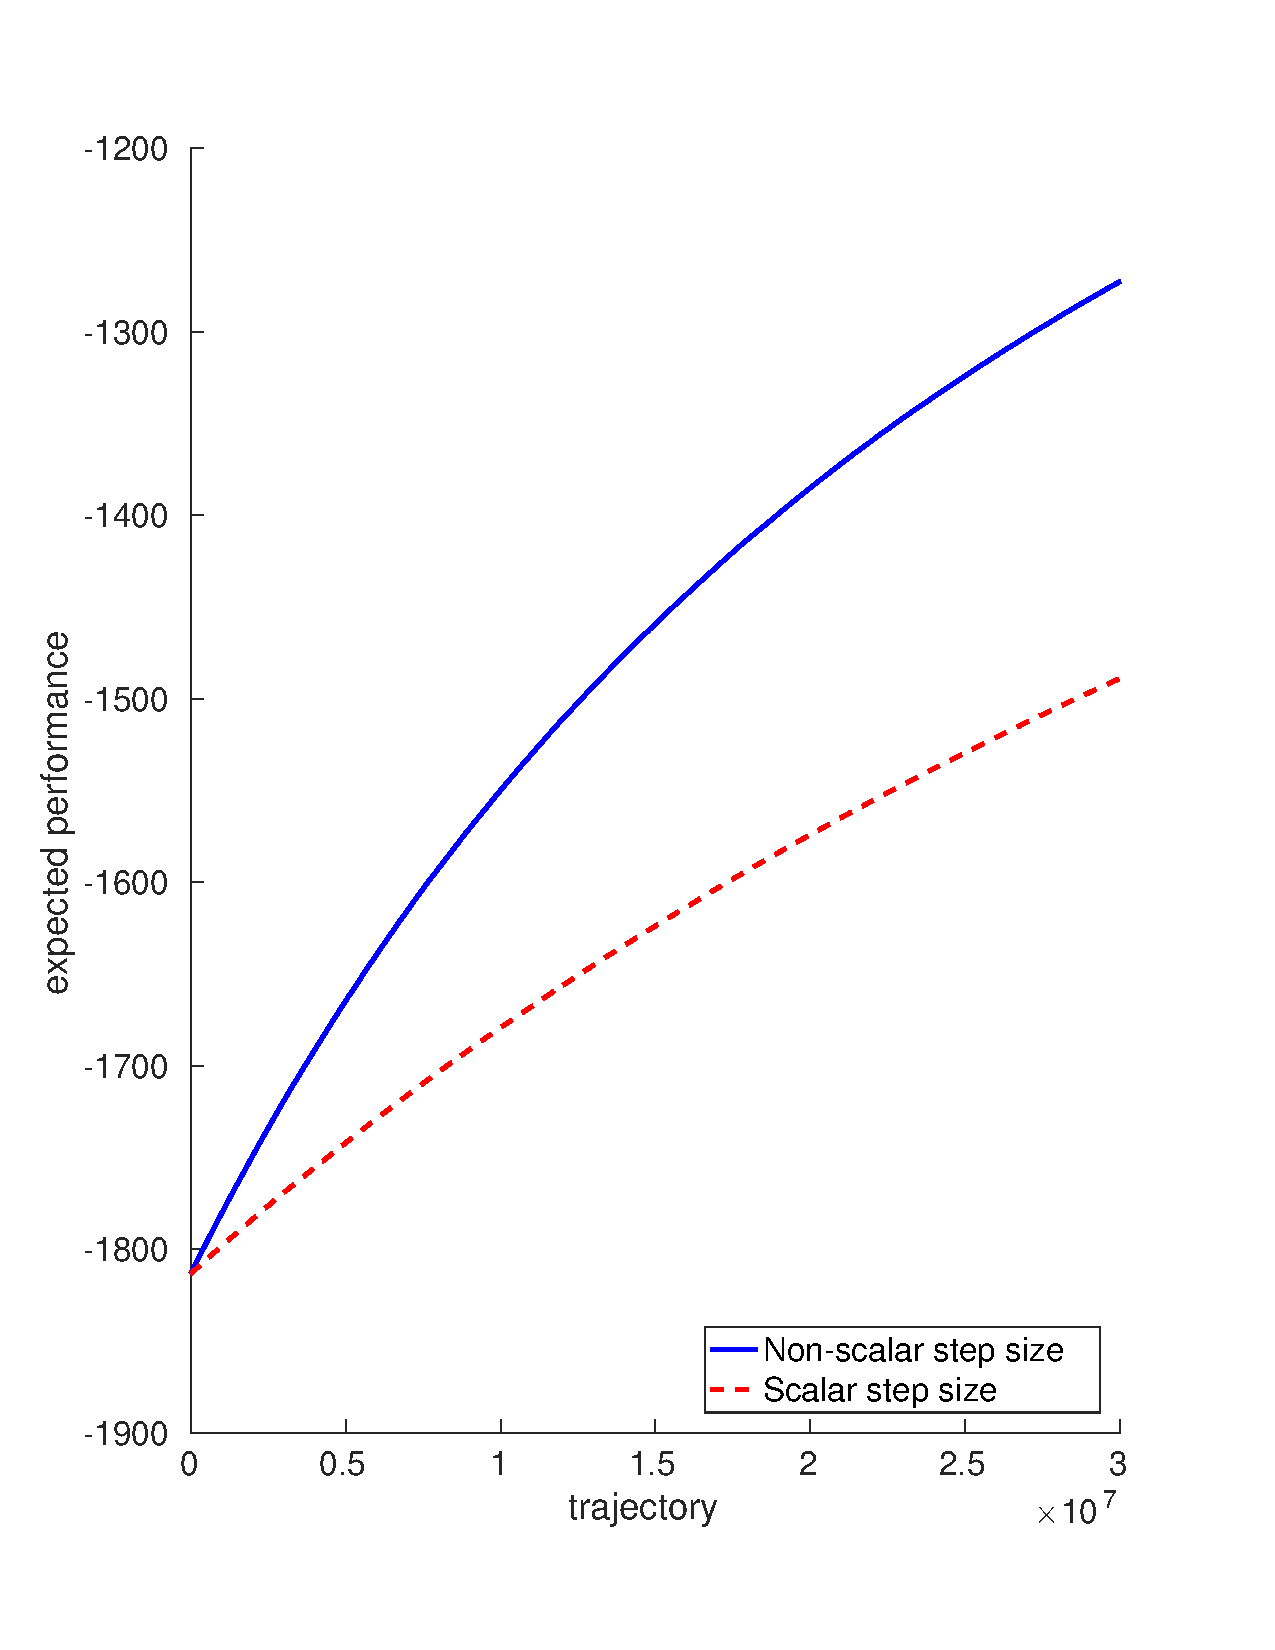
\includegraphics[width=\textwidth,left]{Images/compare_stepsize.pdf}
\caption[Comparison of the performance of the scalar step size and the non-scalar step size.]{Expected performance over sample trajectories in the two-dimensional \ac{LQG} task, using G(PO)MDP, Chebyshev bound, $\delta=0.95$ and fixed $N=2000$. The performance of the adaptive non-scalar step size proposed in this work is compared with the scalar step size from \cite{NIPS2013_5186}, of which the former is a generalization.}
\label{fig:12}
\end{figure}

In both cases, an improvement ratio of 100\% was achieved.
Results on performance show that, indeed, the non-scalar step size outperforms its scalar counterpart.
To get a better insight on how this happens, it is useful to compare the trend of the adaptive step size in the two cases. Figure \ref{fig:13} compares the trend of $\hat{\alpha}^*$ and $\norm{\Lambda^*}$.

\begin{figure}[h!]
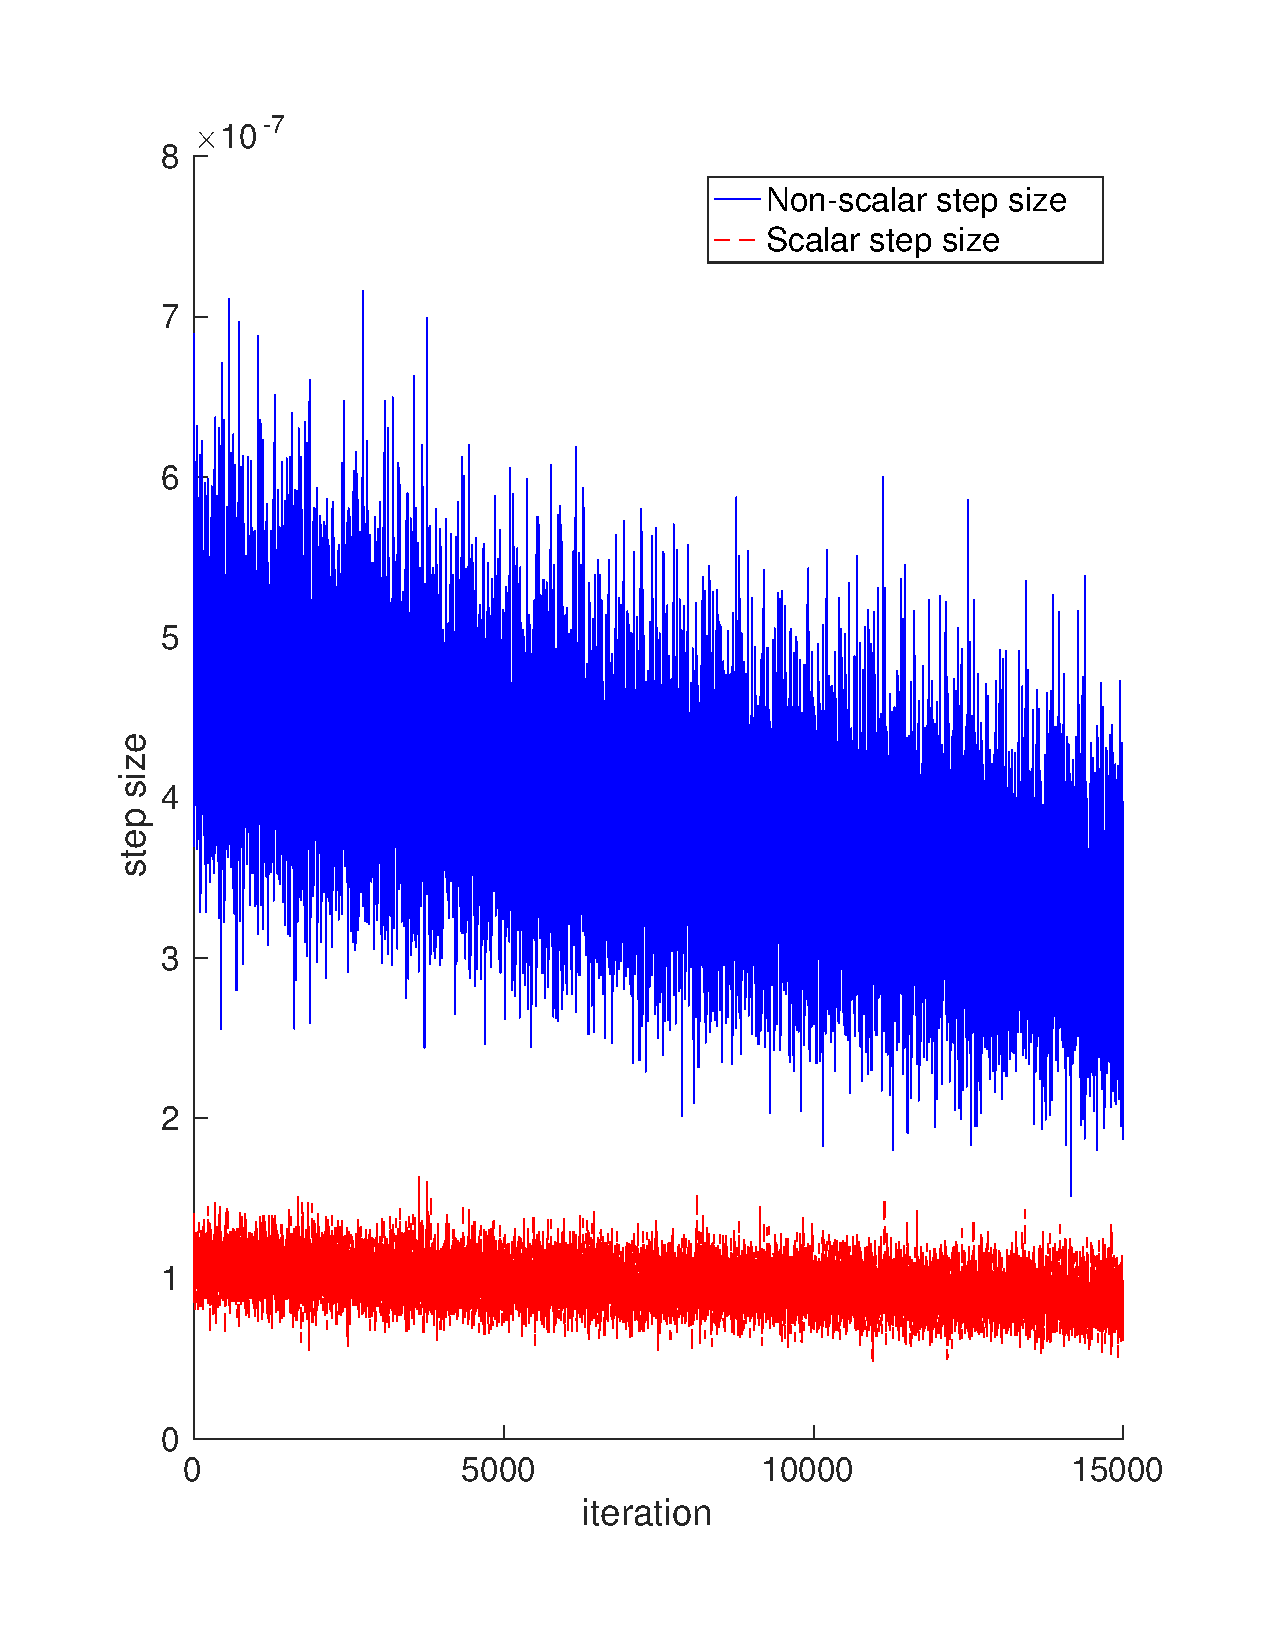
\includegraphics[width=\textwidth,left]{Images/stepsize.pdf}
\caption[Comparison of the trend of scalar and non-scalar step size.]{Magnitude of the step size over learning iterations. The adaptive non-scalar step size proposed in this work is compared with the adaptive scalar step size from \cite{NIPS2013_5186}, of which the former is a generalization.}
\label{fig:13}
\end{figure}

We can see that, although it decreases faster, the non-scalar step size dominates (in magnitude) the scalar one. Basically, the algorithm from \cite{NIPS2013_5186} needs to be more conservative, since more parameters are updated at each learning iteration and their penalties on the guaranteed improvement sum up.

\paragraph{}
Another interesting difference between the two methods is in the shape of the learned policy parameter $\theta$. In any stochastic policy gradient methods, the gradient components relative to $\theta_{12}$ and $\theta_{21}$ are small if compared to the other two, but not zero. This is due to noise and the result is that, even by starting from $\theta = \underline{0}$, the learned parameter will not be a diagonal matrix like the optimal one. On the contrary, a coordinate descent method like ours will never choose to update $\theta_{12}$ or $\theta_{21}$, because the gradient components associated to $\theta_{11}$ and $\theta_{22}$ are much larger. Starting from $\theta = \underline{0}$, a diagonal matrix is obtained.
Although this does not affect performance significantly, it shows how our algorithm is able to completely avoid useless changes in the current policy, which are potential causes of oscillation. In particular, the final parameter obtained with the scalar step size $\hat{\alpha}^*$ was:

\[
\vtheta = \begin{bmatrix}
	-0.014676 & 1.4e-06 \\
	 1.7e-06  & -0.013678
	\end{bmatrix},
\]

while, with our non-scalar step size $\Lambda^*$, we obtained:
\[
\vtheta = \begin{bmatrix}
	-0.0275 & 0 \\
	 0  & -0.0274
	\end{bmatrix},
\]

which is indeed diagonal.

\paragraph{}
We then test our adaptive batch-size on the same task. We use the G(PO)MDP gradient estimator with optimal baseline, Bernstein's bound with empirical range and $\delta=0.95$.
Figure \ref{fig:10} shows the evolution of the batch size over the learning process in the adaptive case.

\begin{figure}[h!]
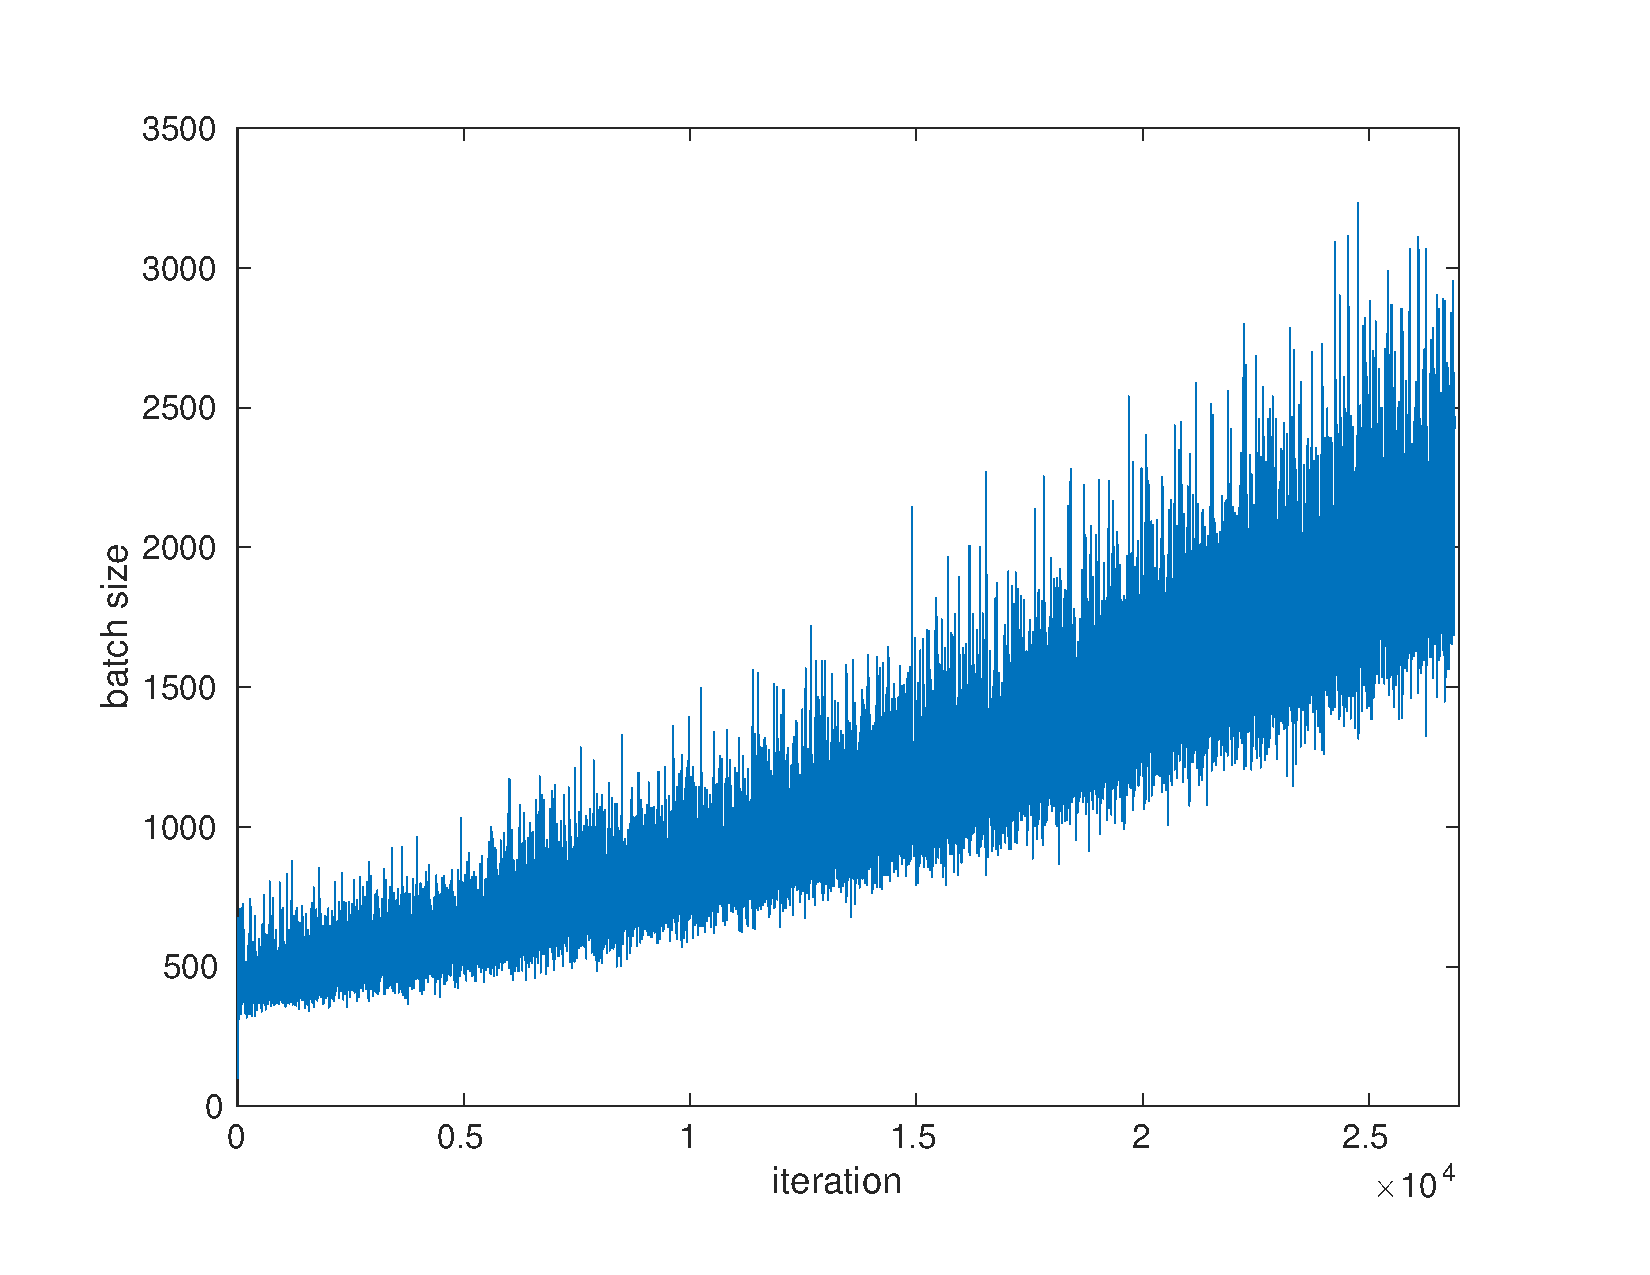
\includegraphics[width = \textwidth,left]{Images/lqg2d_batchsize_landscape.pdf}
\caption[Adaptive batch size over learning iterations in the two-dimensional LQG task.]{Adaptive batch size over learning iterations for the two-dimensional \ac{LQG} task. G(PO)MDP gradient estimator with optimal baseline, Bernstein's bound with empirical range and $\delta=0.95$ were used.}
\label{fig:10}
\end{figure}

The adaptive batch size goes from $N \simeq 500$ in the first learning iterations, to $N\simeq2500$ in the end. The step size takes values of the order of $1e-6$ for the whole process.
We compare the performance of our algorithm with the one of vanilla policy gradient with fixed step size and batch size. Since we want to focus our analysis to the effects of the batch size, we use G(PO)MDP with optimal baseline and $\alpha=1e-6$. We run two simulations, one with $N=1000$ and one with $N=100$. Figure \ref{fig:11} compares expected performance over learning iterations, while table \ref{tab:3} reports average performance $\overline{\Upsilon}$ and improvement ratio for the three cases.

\begin{figure}[h!]
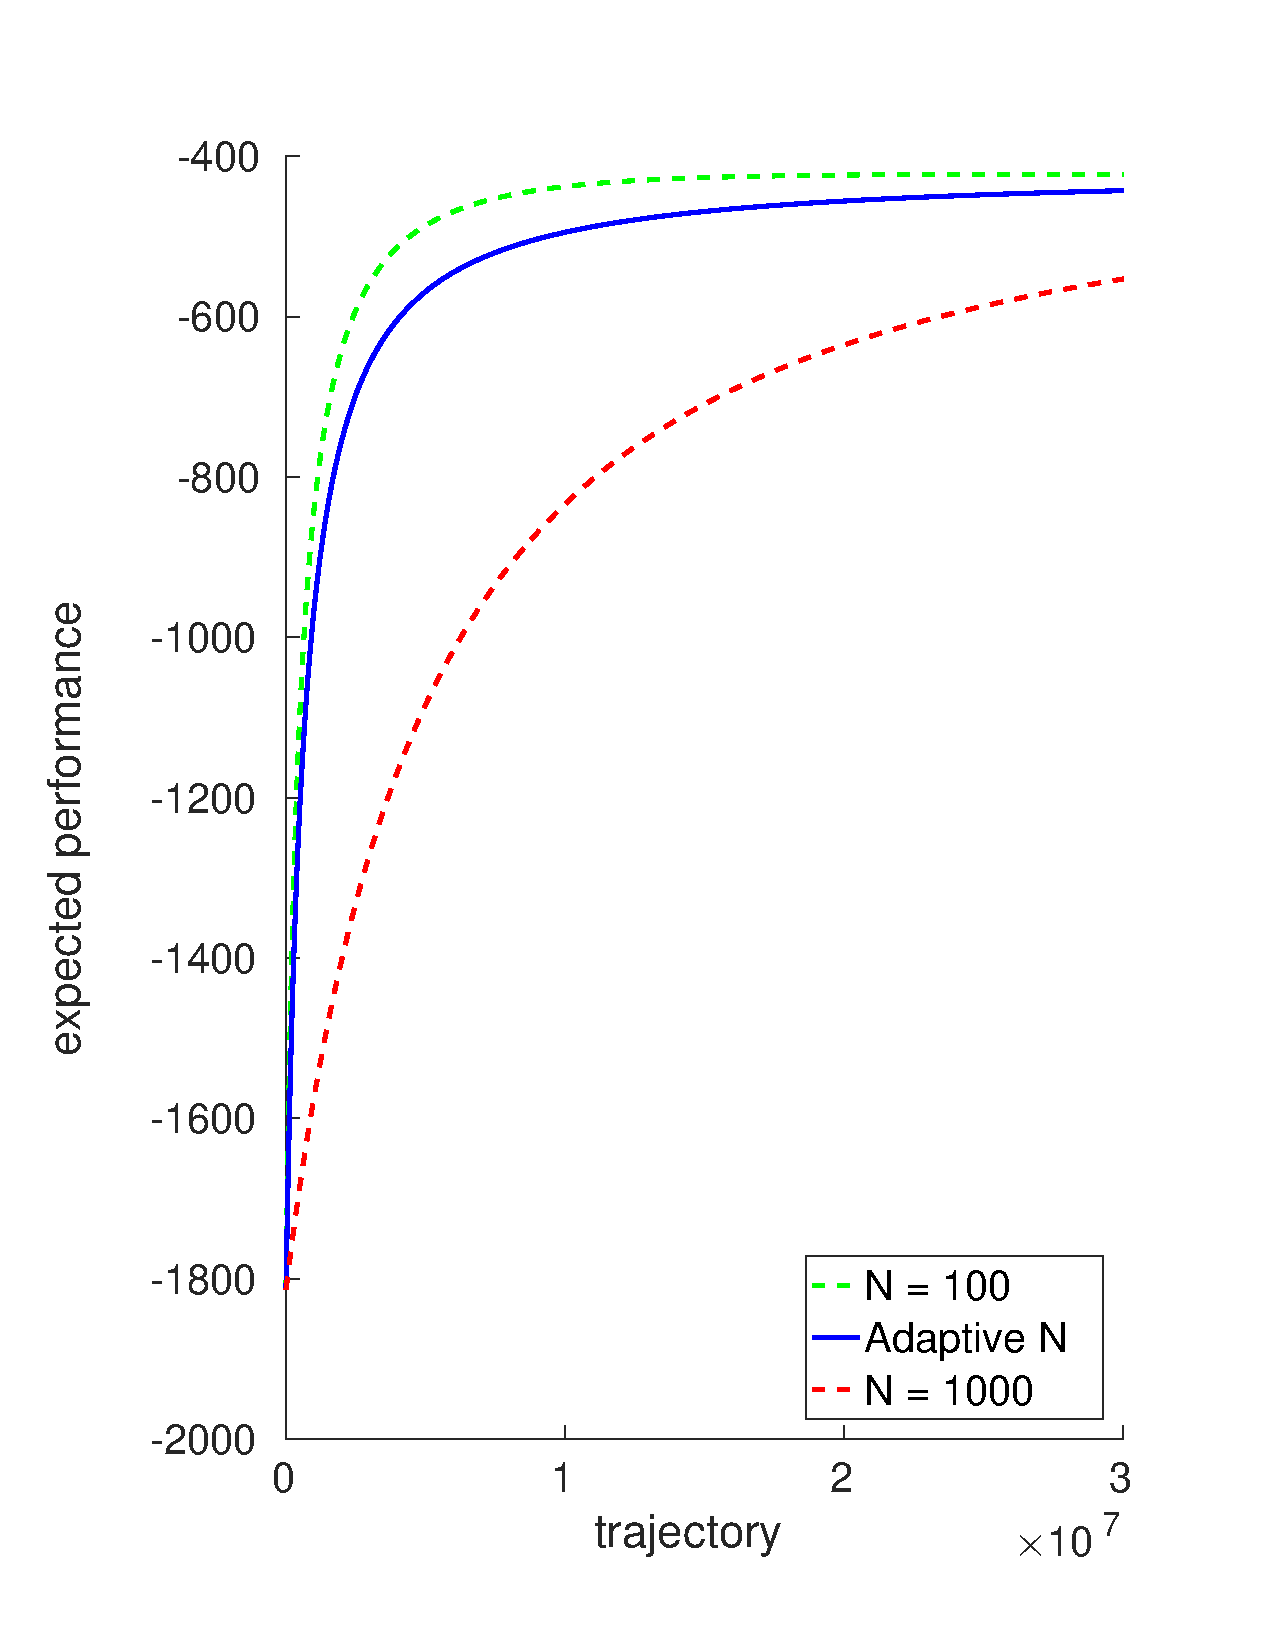
\includegraphics[width = \textwidth]{Images/lqg2d.pdf}
\caption[Expected performance over sample trajectories in the two-dimensional LQG task.]{Expected performance over sample trajectories in the two-dimensional \ac{LQG} task. The adaptive algorithm with Bernstein's bound and $\delta=0.95$ is compared with vanilla policy gradient with fixed $N=100,1000$ and $\alpha=1e-6$.}
\label{fig:11}
\end{figure}

\begin{table}[h!]
\caption[Average performance and improvement ratio for different simulations on the two-dimensional LQG task.]{Average performance and improvement ratio for different simulations on the two-dimensional \ac{LQG} task, using G(PO)MDP. The adaptive batch size is computed using Bernstein's bound with empirical range and $\delta=0.95$. The fixed batch sizes are used in conjunction with $\alpha=1e-6$.}
\label{tab:3}
\centering
\begin{widetable}{\columnwidth}{*{7}{c}} %{@{}lcc@{}} 
\toprule
N & $\overline{\Upsilon}$ & Improvement Ratio \\
\midrule
Adaptive & -20.50 & 100\% \\
1000 & -20.50 & 100\% \\
100 & -19.77 & 0.89\% \\
\bottomrule
\end{widetable}
\end{table}

Results show how a large, fixed batch size can badly affect the convergence rate. Our algorithm is able to outperform the $N=1000$ case by safely employing smaller batch sizes at the beginning of the learning process, turning to larger ones only when it is necessary.
For this task, a small batch size, such as $N=100$, yields a better average performance than our algorithm, but it introduces oscillation, witnessed by a less-than-one improvement ratio.
These results show how an adaptive batch size, such as the one employed by our algorithm, is able to guarantee monotonic improvement without needlessly sacrificing convergence speed.

\section{Cart-Pole}
In this section we test our algorithm on a more challenging simulated control task to give an idea of how it could be useful in practice. We use our algorithm to improve an existing policy after a change has been introduced in the environment, to highlight the advantages of our safe approach.

The cart-pole task is a popular \ac{RL} benchmark problem, of which we use a continuous action variant. An inverted pendulum, the pole, is attached to a cart. A force can be applied to the cart, in order to maintain the pole in a vertical position as long as possible. If the pole becomes too much inclined or the cart goes too far to the left or to the right, the task ends.

In our setting, the cart has a mass of $1Kg$, the pole is $1m$ long and has a mass of $0.1Kg$.
The agent's state is the tuple:
\[
	\boldsymbol{s}_t = [x,\dot{x},\beta,\dot{\beta}],
\]
where $x$ is the position of the cart, $\dot{x}$ is the velocity of the cart, $\beta$ is the angle that the pole forms with the vertical and $\dot{\beta}$ is the angular velocity of the pole. The state is initialized at random in a small neighborhood of $\underline{0}$.
The action is scalar:
\[
	a_t \in [-10,10],
\]
and represents the magnitude of the force applied horizontally to the cart, in newtons.
A constant reward of $1$ is obtained at each time step, such as longer episodes yield better performance. The trajectory has a maximum length of $H=200$ time steps, but it ends as soon as $\beta \notin [-41.8\degree,41.8\degree]$ or $x \notin [-2.4m, 2.4m]$.

We use a Gaussian policy:
\[
	a_t \sim \mathcal{N}(\vtheta^T\boldsymbol{s}_t,\sigma),	
\]
with $\sigma=1$ and starting from $\vtheta=\underline{0}$.

\paragraph{}
We first learn a good policy with a vanilla policy gradient algorithm, using the G(PO)MDP gradient estimator with variance-minimizing baseline, fixed step size $\alpha=0.01$ and batch size $N=4000$. We stop once an average performance of $J_\mu(\vtheta) = 195$ over the batch is achieved. This result is obtained in $72$ iterations. The obtained policy will be referred to as baseline policy.

At this point we introduce a change in the environment, by doubling the length of the pole, keeping its mass constant. If the baseline policy is used in this new setting, the performance immediately drops. Instead, we try to adapt to the change by learning a new policy. This is representative of the scenario presented in Chapter \ref{chap:intro}, where an available policy must be improved to adapt to small changes in the environment.

We run two simulations: the first with the same algorithm used to learn the baseline policy, the second with our adaptive algorithm, using Bernstein's bound with empirical range and $\delta=0.95$.
Figure \ref{fig:14} shows the performance over trajectories of the two approaches (average performance over the batch is used as representative for all the trajectories in the batch), while Table \ref{tab:4} reports average performance and improvement ratio for the two cases. Note that, since the exact value of the expected performance is not available for this task, we are not able to isolate true performance oscillation from noise due to stochasticity in the environment and in the policy itself. However, the improvement ratio computed on the average performance is still indicative of how steadily the policy is improving.

\begin{figure}[h!]
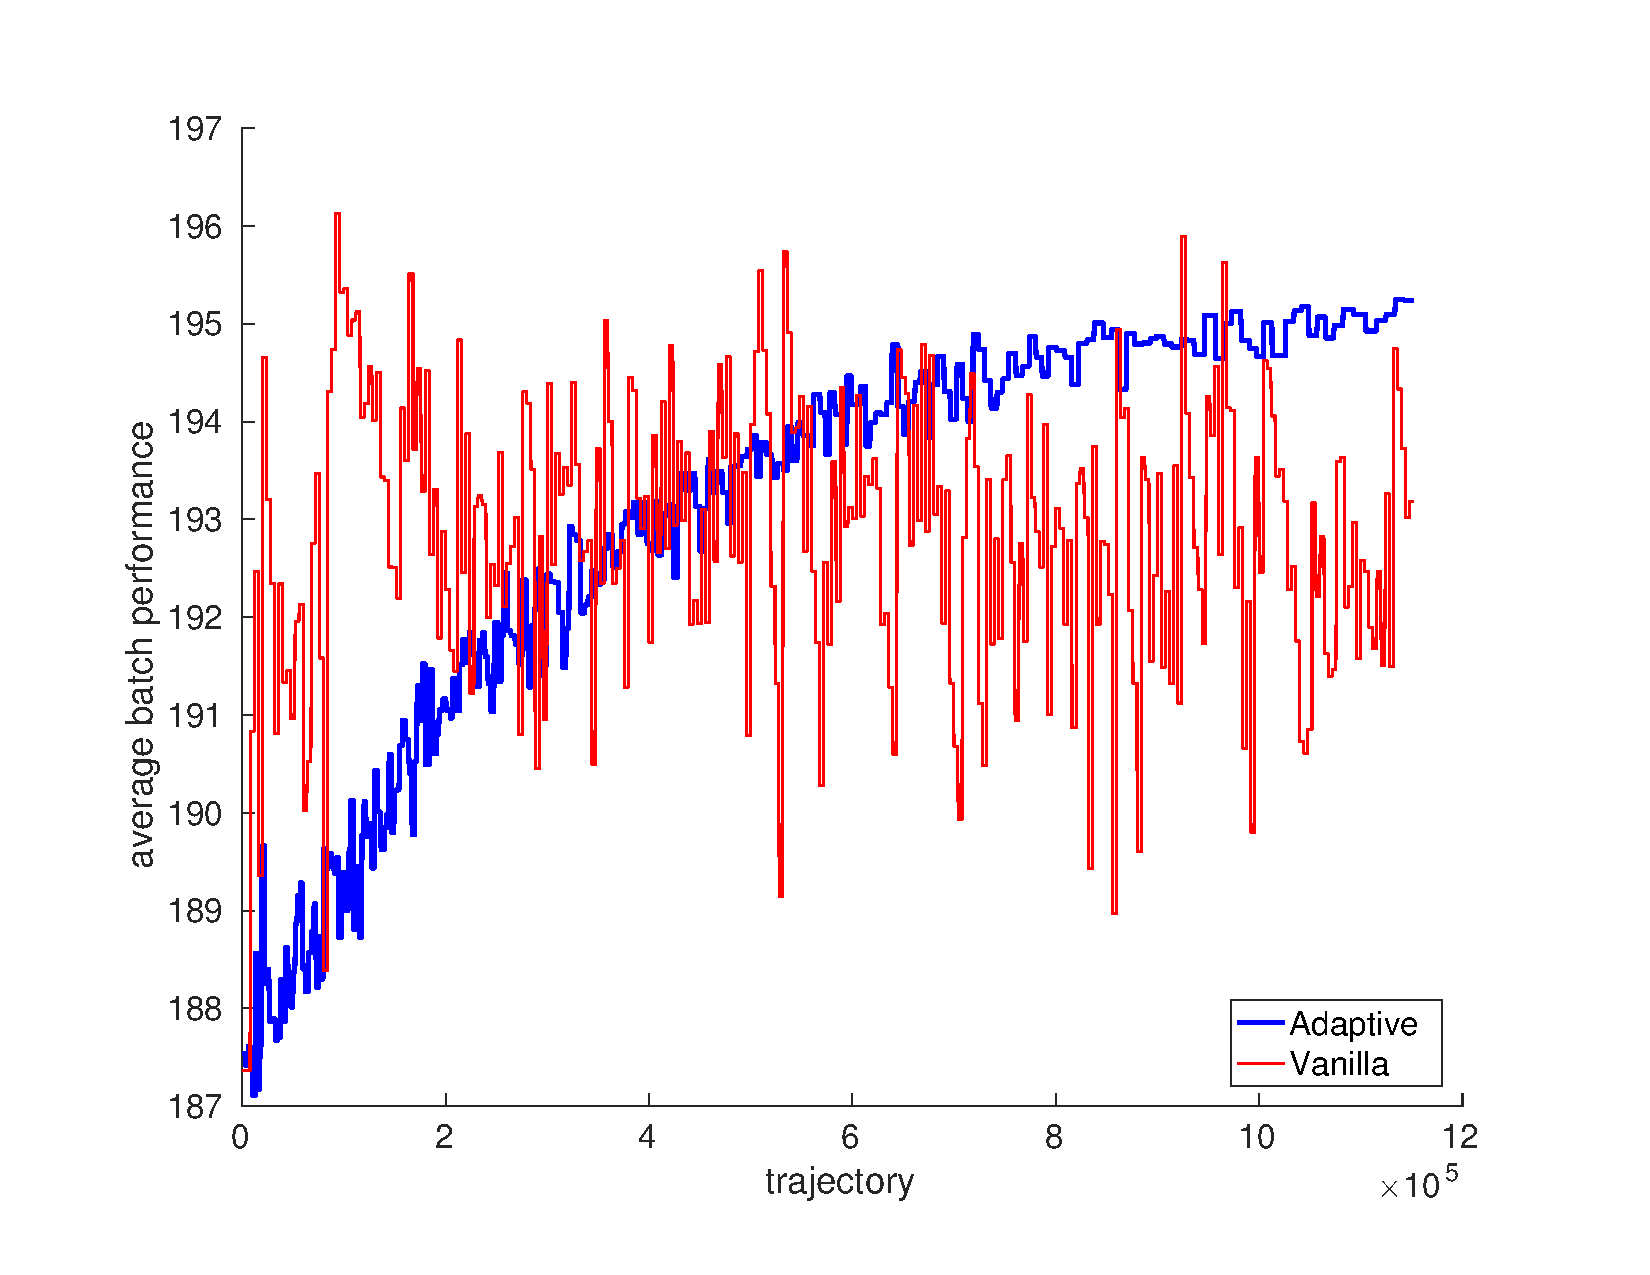
\includegraphics[width = \textwidth]{Images/cartpole.pdf}
\caption[Expected performance over sample trajectories in the cart-pole task.]{Expected performance over sample trajectories in the modified cart-pole task. The adaptive algorithm with Bernstein's bound and $\delta=0.95$ is compared with vanilla policy gradient with fixed $N=4000$ and $\alpha=1e-2$.}
\label{fig:14}
\end{figure}

\begin{table}[h!]
\caption[Average performance and improvement ratio for different simulations on the modified cart-pole task.]{Average performance and improvement ratio for different simulations in the modified cart-pole task, using G(PO)MDP. The adaptive batch size is computed using Bernstein's bound with empirical range and $\delta=0.95$. The fixed batch size is used in conjunction with $\alpha=1e-2$.}
\label{tab:4}
\centering
\begin{widetable}{\columnwidth}{*{7}{c}} %{@{}lcc@{}} 
\toprule
N & $\overline{\Upsilon}$ & Improvement ratio\\ 
\midrule
Adaptive & 193.12 & 53.01\% \\
4000 & 192.86 & 44.76\% \\
\bottomrule
\end{widetable}
\end{table}

Results show how the non-safe approach, although reaching a good performance very quickly, is subject to heavy oscillations, which affect the long term performance. To get the best from this algorithm, a human expert should stop the learning process at the right moment. Instead, our safe algorithm, although taking much longer to reach a good performance, is subject to less oscillations and is able to maintain it indefinitely. This allows for a more autonomous agent, that can react to changes in the environment without any human intervention.

Once again, examining the learned parameters leads to interesting insights: our algorithm never updates the components of $\vtheta$ corresponding to $\beta$ and $\dot{\beta}$, evidently because they are not relevant in adjusting to the particular change that was introduced to the environment. As already observed in Section \ref{sec:lqg2d}, the coordinate descent approach is able to completely avoid some unnecessary sources of oscillation.

\paragraph{}
Although definitely artificial, the cart-pole example shows the possible advantages of employing a safe policy gradient method to a realistic problem, and highlights the main strengths of our proposed algorithm.

	\chapter{Conclusions}
In this thesis we were able to devise an adaptive policy gradient algorithm for Gaussian policies that guarantees monotonic performance improvement with high probability. This algorithm performs coordinate descent and automatically selects both the step size for the parameter updates and the batch size used to collect samples. 

Experiments showed that the algorithm is effective in guaranteeing monotonic improvement, but very conservative in the selection of the batch size. More empirical variants were proposed to address this problem, with satisfying results. However, there is evidence that the method is still quite conservative.
First of all, the worsening probability $\delta$ turned out to have no actual effect on the improvement ratio. Even when values of $\delta$ close to one are selected, the algorithm is conservative enough to avoid oscillation at all. This deprives us of a degree of freedom that could be used to regulate the behavior of the algorithm depending, for instance, on risk aversion or on the degree of non-stationarity of the environment.
Experiments also show how a manually selected batch size can still outperform our method in terms of average performance in many cases. Although small batch sizes do not guarantee monotonic improvement, not always the entity of oscillation has a relevant impact on performance. If we had more control on the wariness of the algorithm, in some applications it would be useful to allow some worsening updates, in order to speed up convergence without compromising long term performance.

Future work could focus on improving the method by devising tighter bounds on the performance improvement.
This would allow to guarantee safety with smaller batches, improving convergence speed, and to gain more control on the degree of safety that needs to be imposed.

The bounds proposed in Section \ref{sec:chebyshev} for the REINFORCE and the G(PO)MDP gradient estimators could be improved by taking into consideration also the effect of variance-minimizing baselines. Additionally, similar ad-hoc bounds could be devised for the other gradient estimation algorithms described in Section \ref{sec:pol_grad}.

Another possibility for future work is to extend the results to more classes of policies. The current approach can be applied only to Gaussian policies with linear expectation and constant standard deviation. Although this kind of policy is broadly used in control tasks, it doesn't cover all the possible applications of policy gradient methods. 
One idea is to generalize the present results, from more complex Gaussian policies to generic parametrized policies.
It would also be useful to adapt the results to other specific classes of policies that are commonly used in practice. For instance, the Softmax policy is a common choice for tasks characterized by a discrete action space. Appendix \ref{app:softmax} shows a first attempt in this direction, highlighting the main difficulties that arise when the approach used for Gaussian policies has to be adapted to the new class.

Other, more ambitious developments may include the analysis of other parameters and their relationship with the ones that have already been considered.
In particular, exploration represents a major problem for policy gradient, as pointed out in \cite{kakade2002approximately}. Including exploration-controlling parameters, such as the standard deviation of the Gaussian policy, in the analysis may lead to faster safe policy gradient algorithms.
	
	% ************************************************************
	% Backmatter
	%*************************************************************
	\cleardoublepage%********************************************************************
% Bibliography
%*******************************************************
% work-around to have small caps also here in the headline
\manualmark
\markboth{\spacedlowsmallcaps{\bibname}}{\spacedlowsmallcaps{\bibname}}
%\phantomsection 
\refstepcounter{dummy} 
% to have the bib a bit from the rest in the toc
\addtocontents{toc}{\protect\vspace{\beforebibskip}}
\addcontentsline{toc}{chapter}{\tocEntry{\bibname}}
\label{app:bibliography} 
\printbibliography
	\appendix
	% \cleardoublepage\part{Appendix}
	\chapter{Proofs}\label{app:proofs}
In this appendix we provide the proofs that were omitted. Some auxiliary lemmas are also introduced and proved.

\begin{lemma}\label{aux:1}
For any initial state distribution $\mu$ and any pair of stationary Gaussian policies $\pi_{\vtheta} \sim \mathcal{N}(\vtheta^T\boldsymbol{\phi}(s),\sigma^2)$ and $\pi_{\vtheta'} \sim \mathcal{N}(\vtheta'^T\boldsymbol{\phi}(s),\sigma^2)$, so that $\vtheta'=\vtheta+\Lambda\gradJ{\vtheta}$, and for any state $s$ and action $a$
\[
\pi(a|s,\vtheta') - \pi(a|s,\vtheta) \geq \nabla_{\vtheta}\pi(a|s,\vtheta)^T\Lambda\gradJ{\vtheta} 
	- \frac{M_{\phi}^2\norm[1]{\Lambda\gradJ{\vtheta}}^2}{\sqrt{2\pi}\sigma^3}
\]
\end{lemma}

\begin{proof}
By exploiting Taylor's expansion
\begin{align*}
\pi(a|s,\vtheta') = & \pi(a|s,\vtheta + \Lambda\gradJ{\vtheta}) = \\
	& \pi(a|s,\vtheta) + \nabla_{\vtheta}\pi(a|s,\vtheta)^T\Delta\vtheta+R_1(\Delta\vtheta),
\end{align*}
where $R_1(\Delta\vtheta)$ is the remainder of the series which can be bounded as follows by exploiting Lemma 4.1 from \cite{NIPS2013_5186} and Assumption 3.1:
\begin{align*}
R_1(\Delta\vtheta) = & \sum\limits_{i=1}^m\sum\limits_{j=1}^m
\frac{\partial^2\pi(a|s,\vtheta)}{\partial\theta_i\partial\theta_j} \bigg|_{\vtheta+c\Delta\vtheta} \frac{\Delta\theta_i\Delta\theta_j}{1+I(i=j)} && \text{for some $c \in (0,1)$} \\
	\geq & - \sum\limits_{i=1}^m\sum\limits_{j=1}^m \frac{|\phi_i(s)\phi_j(s)|}{\sqrt{2\pi}\sigma^3}
	\frac{\Delta\theta_i\Delta\theta_j}{1+I(i=j)} \\
	= & -\frac{1}{\sqrt{2\pi}\sigma^3}\sum\limits_{i=1}^m\sum\limits_{j=1}^m
	\frac{\alpha_i|\phi_i(s)|\gradJ{\theta_i}\alpha_j|\phi_j(s)|\gradJ{\theta_j}}{1+I(i=j)} \\
	= & - \frac{(|\gradJ{\vtheta}|^T\Lambda|\vphi(s)|)^2}{\sqrt{2\pi}\sigma^3} \\
	\geq & - \frac{M_{\phi}^2\norm[1]{\Lambda\gradJ{\vtheta}}^2}{\sqrt{2\pi}\sigma^3}.
\end{align*}
It is now enough to apply this bound to Taylor's expansion.
\end{proof}

\begin{lemma}\label{aux:2}
For any initial state distribution $\mu$ and any pair of stationary Gaussian policies $\pi_{\vtheta} \sim \mathcal{N}(\vtheta^T\boldsymbol{\phi}(s),\sigma^2)$ and $\pi_{\vtheta'} \sim \mathcal{N}(\vtheta'^T\boldsymbol{\phi}(s),\sigma^2)$, so that $\vtheta'=\vtheta+\Lambda\gradJ{\vtheta}$

\[ \norm[\infty]{\pi_{\vtheta'}-\pi_{\vtheta}}^2 \leq \
	\frac{M_{\phi}^2\norm[1]{\Lambda\gradJ{\vtheta}}^2}{\sigma^2}
\]
\end{lemma}

\begin{proof}
By exploiting Pinsker's inequality \cite{Pinsker1960}
\begin{align*}
\norm[\infty]{\pi_{\vtheta'}-\pi_{\vtheta}}^2 = & \sup\limits_s \norm[\infty]{\pi_{\vtheta'}-\pi_{\vtheta}}^2 \\
	\geq & \sup\limits_s 2H(\pi_{\vtheta'}||\pi_{\vtheta}) \\
	= & \sup\limits_s \frac{1}{\sigma^2} \sum\limits_i 
	(\gradJ{\theta_i}\alpha_i\phi_i(s))^2 \\
	\geq & \frac{M_{\phi}^2\norm[1]{\Lambda\gradJ{\vtheta}}^2}{\sigma^2},
\end{align*}
where $H(P||Q)$ is the Kullback-Liebler divergence.
\end{proof}


\firstlemma*
\begin{proof}
We plug the results of Lemmas \ref{aux:1} and \ref{aux:2} into Lemma 3.1 from \cite{NIPS2013_5186}:
\begin{align*}
J_{\mu}(\vtheta') - J_{\mu}(\vtheta) \geq  
	& \frac{1}{1-\gamma} \int_{\mathcal{S}}d_{\mu}^{\pi_{\vtheta}}(s)
	\int_{\mathcal{A}} (\pi(a|s,\vtheta') - \pi(a|s,\vtheta))Q^{\pi_{\vtheta}}(s,a)\mathrm{d}a\mathrm{d}s \\
	& -\frac{\gamma}{2(1-\gamma)^2} \norm[\infty]{\pi_{\vtheta'}-\pi_{\vtheta}}^2 \norm[\infty]{Q^{\pi_{\vtheta}}} \\
	\geq & 
		\frac{1}{1-\gamma} \int_{\mathcal{S}}d_{\mu}^{\pi_{\vtheta}}(s)
		\int_{\mathcal{A}}
		\nabla_{\vtheta}\pi(a|s,\vtheta)^T\Lambda\gradJ{\vtheta}
		Q^{\pi_{\vtheta}}(s,a)\mathrm{d}a\mathrm{d}s && (1) \\
		& - \frac{M_{\phi}^2\norm[1]{\Lambda\gradJ{\vtheta}}^2}
		{(1-\gamma)\sqrt{2\pi}\sigma^3}
		\int_{\mathcal{S}}d_{\mu}^{\pi_{\vtheta}}(s)
		\int_{\mathcal{A}} 
		Q^{\pi_{\vtheta}}(s,a)\mathrm{d}a\mathrm{d}s && (2) \\ 
		&  -\frac{\gamma M_{\phi}^2\norm[1]{\Lambda\gradJ{\vtheta}}^2}
		{2(1-\gamma)^2\sigma^2}\norm[\infty]{Q^{\pi_{\vtheta}}}	&& (3)
\end{align*}
Term $(1)$ can be simplified by using the Policy Gradient Theorem \cite{NIPS1999_1713}:
\begin{align*}
\frac{1}{1-\gamma} &  \int_{\mathcal{S}}d_{\mu}^{\pi_{\vtheta}}(s)
		\int_{\mathcal{A}}
		\nabla_{\vtheta}\pi(a|s,\vtheta)^T\Lambda\gradJ{\vtheta}
		Q^{\pi_{\vtheta}}(s,a)\mathrm{d}a\mathrm{d}s \\
		= & \frac{\gradJ{\vtheta}^T\Lambda}{1-\gamma}
		\int_{\mathcal{S}}d_{\mu}^{\pi_{\vtheta}}(s)
		\int_{\mathcal{A}}
		\nabla_{\vtheta}\pi(a|s,\vtheta)Q^{\pi_{\vtheta}}(s,a)\mathrm{d}a\mathrm{d}s \\
		= & \gradJ{\vtheta}^T\Lambda\gradJ{\vtheta}
\end{align*}
The proof now follows simply by rearranging terms.
\end{proof}


% \paragraph{Theorem \ref{theo:1}}
\firsttheorem*
\begin{proof}
For every state $s \in \mathcal{S}$ and every action $a \in \mathcal{A}$, the Q-function belongs to $\left[-\frac{R}{1-\gamma},\frac{R}{1-\gamma}\right]$. As a consequence, $\int_{\mathcal{A}}Q^{\pi_{\vtheta}}(s,a)\mathrm{d}a \leq \frac{|\mathcal{A}|R}{1-\gamma}$ and $\norm[\infty]{Q^{\pi_{\vtheta}}} \leq \frac{R}{1-\gamma}$. The proof follows from applying these bounds to the expression of Lemma \ref{lemma:1}.
\end{proof}

% \paragraph{Theorem \ref{theo:3}}
\thirdtheorem*
\begin{proof}
The proof immediately follows from Theorem 3.3 and the definition of $\gradDown{\vtheta}$ and $\gradUp{\vtheta}$. Note that the saturation to $0$ in $\gradDown{\vtheta}$ is necessary since $\gradJ{\vtheta}$ is taken with absolute value in the negative term of the original bound.
\end{proof}

\paragraph{Theorem \ref{theo:5}}
% {\fourththeorem*}
\begin{proof}
We first optimize the cost function $\Upsilon_{\delta}$ w.r.t $\Lambda$. Since $\Upsilon_{\delta}$ is just the bound from Theorem \ref{theo:3} divided by $N$, we can use the result from Corollary \ref{cor:3}, which under Assumption \ref{assum:4} can be expressed as:
\[
\alpha_k^* = 
\begin{cases}
	\frac{
		\left(\norm[\infty]{\gradApp{\vtheta}} - \nicefrac{d_{\delta}}{\sqrt{N}}\right)^2}
		{2c
		\left(\norm[\infty]{\gradApp{\vtheta}} + \nicefrac{d_{\delta}}{\sqrt{N}}\right)^2} & 
		\text{if } k = \arg\max_i |\gradApp{\theta_i}|,	\\
		0 & \text{otherwise},
\end{cases}
\]
which yields:
\[
	\Upsilon_{\delta}(\Lambda^*,N) = 
	\frac{
		\left(\norm[\infty]{\gradApp{\vtheta}} - \nicefrac{d_{\delta}}{\sqrt{N}}\right)^4}
		{4c
		\left(\norm[\infty]{\gradApp{\vtheta}} + \nicefrac{d_{\delta}}{\sqrt{N}}\right)^2N}.
\]
To justify the use of Corollary \ref{cor:3}, our $N^*$ must be compliant with \ref{assum:3}, which, under Assumption \ref{assum:4}, translates into the following constraint:
\[
N \geq N_0 := \frac{d_{\delta}^2}{\norm[\infty]{\gradApp{\vtheta}}^2}.
\] 
By computing the derivative $\nicefrac{\partial\Upsilon_{\delta}}{\partial N}$ we find just two stationary points in $[N_0,+\infty)$: the first one is $N_0$ itself, which is a minimum ($\Upsilon_{\delta}(\Lambda^*,N_0) = 0$ and $\Upsilon_{\delta}$ is non-negative); the other one is our optimal batch size:
\[
	N^* =  \frac{(13+3\sqrt{17})d_{\delta}^2}{2\norm[\infty]{\gradApp{\vtheta}}^2}.
\]
Since $\Upsilon_{\delta}(\Lambda^*,N_1)=0, \lim\limits_{N \to +\infty}\Upsilon_{\delta} (\Lambda^*,N)= 0$, and $\Upsilon_{\delta}$ is continuous and differentiable in $[N_0,+\infty)$, $N^*$ is indeed the global maximum in the region of interest. We can now substitute $N^*$ into $\Lambda^*$ to obtain:
\begin{align*}
&\alpha_k^* = 
\begin{cases}  
	\frac{(13-3\sqrt{17})}
		{4c} & 
		\text{if } k = \arg\max\limits_i |\gradApp{\theta_i}|,	\\
		0 & \text{otherwise},
\end{cases}
\end{align*}
and into $\Upsilon_{\delta}(\Lambda^*,N^*)$ to obtain:
\[
	\Upsilon^* = \frac{(4977-1207\sqrt{17})\norm[\infty]{\gradApp{\vtheta}}^4}{32d_{\delta}^2}.
\]
Finally
\[
	\DeltaJ \geq N^*\Upsilon^* 
	= \frac{393-95\sqrt{17}}{8}\norm[\infty]{\gradApp{\vtheta}}^2
\]

with probability at least $(1-\delta)^m$.

\end{proof}


% \paragraph{Lemma \ref{lemma:2}}
\secondlemma*
\begin{proof}
We focus on the REINFORCE\cite{Williams1992} gradient estimator:
\[
\hat{\nabla}_{\vtheta}J_{\mu}^{RF}(\vtheta) = 
	\frac{1}{N}\sum\limits_{n=1}^N\left(
	\sum\limits_{k=1}^H\nabla_{\vtheta}\log\pi(a_k^n|s_k^n,\vtheta)
	\left(\sum\limits_{l=1}^H\gamma^{l-1}r_l^n-b\right)\right),
\]
and the G(PO)MDP\cite{bb-ihgbps-01}/PGT\cite{Sutton1999a} gradient estimator:
\[
\gradPGT{\vtheta} = \gradGPOMDP{\vtheta} = 
	\frac{1}{N}\sum\limits_{n=1}^N\left(
	\sum\limits_{k=1}^H\nabla_{\vtheta}\log\pi(a_k^n|s_k^n,\vtheta)
	\left(\sum\limits_{l=k}^H\gamma^{l-1}r_l^n-b_l^n\right)\right).
\]
In both cases, the i-th component of the single sample can be bounded in absolute value as
\[
\sum\limits_{k=1}^H\nabla_{\theta_i}|\log\pi(a_k^n|s_k^n,\vtheta)|\frac{R}{1-\gamma}.
\]
In the case of Gaussian policy, bounded action space ($|a| \leq \overline{A}$) and under Assumption \ref{assum:1}, in the most general case, the range of the term $\nabla_{\theta_i}\log\pi(a_k^n|s_k^n,\vtheta)$ can be bounded as
\[
\frac{2M_{\phi}\overline{A}}{\sigma^2}.
\] 
Finally
\[
\mathbf{R} \leq \frac{2HM_{\phi}\overline{A}R}{\sigma^2(1-\gamma)}
\]
\end{proof}
	\chapter{Extension to Softmax Policies}\label{app:softmax}

In this appendix we show a first attempt at adapting the results on monotonic improvement to the class of Softmax Policies, as suggested in Chapter 6. The impractical nature of this partial results is indicative of the difficulties that characterize this task and could be useful to guide future research on the matter.
\paragraph{}
We fist need some Lemmas about specific properties of Softmax policies:

\begin{lemma}\label{lem:softmax_d2}
If $\pi_{\vtheta}$ is a softmax policy:
\[
\left| \frac{\partial^2\pi_{\vtheta}(a \mid s)}
	{\partial\theta_i\partial\theta_j}\right| \leq
	6M_{\phi}^2.
\]
\end{lemma}
\begin{proof}
\begin{align*}
\left|\frac{\partial^2\pi_{\vtheta}(a \mid s)}
		{\partial\theta_i\partial\theta_j}\right|
		&= \left| \pi_{\vtheta}(a\mid s)\left(
		\phi_j(s,\cdot)\phi_i(s,\cdot) -  \phi_i(s,\cdot)\expected{a'}{\pi_{\vtheta}}{\phi_j(s,\cdot)} - \phi_j(s,\cdot)\expected{a'}{\pi_{\vtheta}}{\phi_i(s,\cdot)}\right.\right. \\
		&\left.\left.+ 2\expected{a'}{\pi_{\vtheta}}{\phi_i(s,\cdot)}\expected{a'}{\pi_{\vtheta}}{\phi_j(s,\cdot)} - \expected{a'}{\pi_{\vtheta}}{\phi_i(s,\cdot)\phi_j(s,\cdot)}\right)\right| \\
		\leq 6M_\phi^2.
\end{align*}
\end{proof}

\begin{lemma}\label{lem:softmax_diff}
If $\pi_{\vtheta}$ is a softmax policy and $\vtheta' = \vtheta+\Lambda\gradJ{\vtheta}$:
\[
\pi_{\vtheta'}(a \mid s) - \pi_{\vtheta}(a \mid s) \geq 
	\nabla_{\vtheta}\pi_{\vtheta}(a \mid s)^T\Lambda\gradJ{\vtheta} -
	6M_{\phi}^2\norm[1]{\Lambda\gradJ{\vtheta}}^2.
\]
\end{lemma}
\begin{proof}
It follows from the application of Lemma \ref{lem:softmax_d2} to Taylor's expansion.
\end{proof}

\begin{lemma}\label{lem:softmax_infnorm}
If $\pi_{\vtheta}$ is a softmax policy and $\vtheta' = \vtheta+\Lambda\gradJ{\vtheta}$:
\[
	\norm[\infty]{\pi_{\vtheta'} - \pi_{\vtheta}}^2 \leq 4M_\phi\norm[1]{\Lambda\gradJ{\vtheta}}.
\]
\end{lemma}
\begin{proof}
By Pinsker's inequality:
\begin{align*}
\norm[\infty]{\pi_{\vtheta'} - \pi_{\vtheta}}^2 = \sup_s\norm[1]{\pi_{\vtheta'} - \pi_{\vtheta}}^2 \leq \sup_s\left(2H(\pi_{\vtheta'}\mid\mid\pi_{\vtheta})\right),
\end{align*}
where $H(\cdot\mid\mid\cdot)$ is the Kullback-Liebler divergence, which in this case can be bounded as:
\begin{align*}
H(\pi_{\vtheta'},\pi_{\vtheta}) &= 
\sum_{a \in \mathcal{A}}
	\frac{e^{\vtheta'^T\phi(s,a)}}{\sum_{a'\in\mathcal{A}}e^{\vtheta'^T\phi(s,a')}}
	\log\frac{e^{\vtheta'^T\phi(s,a)}\sum_{a'\in\mathcal{A}}e^{\vtheta^T\phi(s,a')}}
	{e^{\vtheta^T\phi(s,a)}\sum_{a'\in\mathcal{A}}e^{\vtheta'^T\phi(s,a')}} \\
	&= \expected{a}{\pi_{\vtheta'}}{
	\Delta\vtheta^T\phi(s,a) + \log\frac{\sum_{a'\in\mathcal{A}}e^{\vtheta^T\phi(s,a')}}
	{\sum_{a'\in\mathcal{A}}e^{\vtheta'^T\phi(s,a')}}} \\
	&= \expected{a}{\pi_{\vtheta'}}{
	\Delta\vtheta^T\phi(s,a) + \log\frac{\sum_{a'\in\mathcal{A}}e^{\vtheta^T\phi(s,a')}}		{\sum_{a'\in\mathcal{A}}e^{\vtheta^T\phi(s,a')}e^{\Delta\vtheta^T\phi(s,a')}}} \\
	&\leq \expected{a}{\pi_{\vtheta'}}{
	\norm[1]{\Delta\vtheta}M_\phi + \log\frac{\cancel{\sum_{a'\in\mathcal{A}}e^{\vtheta^T\phi(s,a')}}}
	{e^{-\norm[1]{\Delta\vtheta}M_\phi}\cancel{\sum_{a'\in\mathcal{A}}e^{\vtheta^T\phi(s,a')}}}} \\
	&= 2\norm[1]{\Delta\vtheta}M_\phi = 2M_\phi\norm[1]{\Lambda\gradJ{\vtheta}}. 	
\end{align*}
The rest of the proof is trivial.
\end{proof}

We can now state the following theorem, which is a variant of Theorem \ref{theo:1}

\begin{theorem}\label{theo:softmax1}
For any initial state distribution $\mu$, if $\pi_{\vtheta}$ is a softmax policy and $\vtheta' = \vtheta+\Lambda\gradJ{\vtheta}$:
\begin{align*}
\DeltaJ &\geq \gradJ{\vtheta}^T\Lambda\gradJ{\vtheta} \\
	&-c\norm[1]{\Lambda\gradJ{\vtheta}}^2 -
	b\norm[1]{\Lambda\gradJ{\vtheta}},
\end{align*}
where
\begin{align*}
c &= \frac{6M_{\phi}^2|\mathcal{A}|R}{(1-\gamma)^2}, \\
b &=  \frac{2\gamma M_{\phi}R}{(1-\gamma)^3}.
\end{align*}
\end{theorem}
\begin{proof}
It's enough to plug the results from Lemmas \ref{lem:softmax_diff} and \ref{lem:softmax_d2} into Lemma 3.1 from \cite{NIPS2013_5186}.
\end{proof}

\begin{corollary}\label{cor:softmax_stepsize}
The performance lower bound of Theorem \ref{theo:softmax1} is maximized, under the assumption that $b\leq \norm[\infty]{\gradJ{\vtheta}}$, by the following non-scalar step size:
\[ \alpha_{k}^*=	
\begin{cases}
	\frac{1}
		{2c}\left(1-\frac{b}{\norm[\infty]{\gradJ{\vtheta}}}\right) & 
		\text{if } k = \arg\max\limits_i |\gradJ{\theta_i}|,	\\
		0 & \text{otherwise},
\end{cases}
\]
which guarantees the following performance improvement: 
\[
\DeltaJ \geq \frac{\left(\norm[\infty]{\gradJ{\vtheta}} - b\right)^2}{4c}.
\]
\end{corollary}
\begin{proof}
The proof is very similar to the one of Corollary \ref{cor:1}, so we omit it.
\end{proof}

The issue with the result of Corollary \ref{cor:softmax_stepsize} is that, in practical applications, the constant $b$ can easily be larger than $\norm[\infty]{\gradJ{\vtheta}}$. This means that, in many cases, no improvement-guaranteeing step size can be found, not even when the policy gradient is known exactly.
Although this result cannot be used in practice, it shows that the main difficulty in extending our method to Softmax policies is the characterization of the policy difference measure $\norm[\infty]{\pi_{\vtheta'} - \pi_{\vtheta}}^2$. Further research should be aimed at overcoming or bypassing this issue.
	

\end{document}
% ****************************************************************